\PassOptionsToPackage{enable-debug,check-declarations}{expl3}
\RequirePackage{pdfmanagement-testphase}
\DeclareDocumentMetadata {  }
\ExplSyntaxOn
\pdfmanagement_add:nnn{Catalog}{Lang}{(enUS)}
\ExplSyntaxOff

% xmp metadata for pdf
% Originally used \usepackage[a-2a]{pdfx}
% \usepackage{hyperxmp} replaced it
% \RequirePackage{pdfmanagement-testphase} replaced it

\documentclass[11pt,
  english,
  a4paper,
]{article}
\usepackage{sa4ss}
\usepackage{amsmath,amssymb,array}
\usepackage{booktabs}

% From tagged-template.latex
\usepackage{lmodern}
\usepackage{ifxetex,ifluatex}
\ifnum 0\ifxetex 1\fi\ifluatex 1\fi=0 % if pdftex
  \usepackage[T1]{fontenc}
  \usepackage[utf8]{inputenc}
  \usepackage{textcomp} % provide euro and other symbols
\else % if luatex or xetex
  \usepackage{unicode-math}
  \defaultfontfeatures{Scale=MatchLowercase}
  \defaultfontfeatures[\rmfamily]{Ligatures=TeX,Scale=1}
\fi

% Use upquote if available, for straight quotes in verbatim environments
\IfFileExists{upquote.sty}{\usepackage{upquote}}{}
\IfFileExists{microtype.sty}{% use microtype if available
  \usepackage[]{microtype}
  \UseMicrotypeSet[protrusion]{basicmath} % disable protrusion for tt fonts
}{}
\makeatletter
\@ifundefined{KOMAClassName}{% if non-KOMA class
  \IfFileExists{parskip.sty}{%
    \usepackage{parskip}
  }{% else
    \setlength{\parindent}{0pt}
    \setlength{\parskip}{6pt plus 2pt minus 1pt}}
}{% if KOMA class
  \KOMAoptions{parskip=half}}
\makeatother
\usepackage{xcolor}
\IfFileExists{xurl.sty}{\usepackage{xurl}}{} % add URL line breaks if available
\hypersetup{
  pdftitle={DRAFT Stock Assessment of the Squarespot Rockfish (Sebastes hopkinsi) along the California U.S. West Coast in 2021 using catch, length, and fishery-independent abundance data},
  pdflang={en},
  hidelinks,
  pdfcreator={LaTeX via pandoc}}
\urlstyle{same} % disable monospaced font for URLs
\usepackage{longtable}
% Correct order of tables after \paragraph or \subparagraph
\usepackage{etoolbox}
\makeatletter
\patchcmd\longtable{\par}{\if@noskipsec\mbox{}\fi\par}{}{}
\makeatother
% Allow footnotes in longtable head/foot
\IfFileExists{footnotehyper.sty}{\usepackage{footnotehyper}}{\usepackage{footnote}}
\makesavenoteenv{longtable}
\usepackage{graphicx}
\makeatletter
\def\maxwidth{\ifdim\Gin@nat@width>\linewidth\linewidth\else\Gin@nat@width\fi}
\def\maxheight{\ifdim\Gin@nat@height>\textheight\textheight\else\Gin@nat@height\fi}
\makeatother
% Scale images if necessary, so that they will not overflow the page
% margins by default, and it is still possible to overwrite the defaults
% using explicit options in \includegraphics[width, height, ...]{}
\setkeys{Gin}{width=\maxwidth,height=\maxheight,keepaspectratio}
% Set default figure placement to htbp
\makeatletter
\def\fps@figure{htbp}
\makeatother
\setlength{\emergencystretch}{3em} % prevent overfull lines
\providecommand{\tightlist}{%
  \setlength{\itemsep}{0pt}\setlength{\parskip}{0pt}}
\setcounter{secnumdepth}{5}
\ifxetex
  % Load polyglossia as late as possible: uses bidi with RTL langages (e.g. Hebrew, Arabic)
  \usepackage{polyglossia}
  \setmainlanguage[]{english}
\else
  \usepackage[shorthands=off,main=english]{babel}
\fi

%Define cslreferences environment, required by pandoc 2.8
%https://github.com/rstudio/rmarkdown/issues/1649
\newlength{\csllabelwidth}
\setlength{\csllabelwidth}{3em}
\newlength{\cslhangindent}
\setlength{\cslhangindent}{1.5em}
% for Pandoc 2.8 to 2.10.1
\newenvironment{cslreferences}%
  {}%
  {\par}
% For Pandoc 2.11+
\newenvironment{CSLReferences}[2] % #1 hanging-ident, #2 entry spacing
 {% don't indent paragraphs
  \setlength{\parindent}{0pt}
  % turn on hanging indent if param 1 is 1
  \ifodd #1 \everypar{\setlength{\hangindent}{\cslhangindent}}\ignorespaces\fi
  % set entry spacing
  \ifnum #2 > 0
  \setlength{\parskip}{#2\baselineskip}
  \fi
 }%
 {}
\usepackage{calc}  % for \widthof, \maxof in minipage
\newcommand{\CSLBlock}[1]{#1\hfill\break}
\newcommand{\CSLLeftMargin}[1]{\parbox[t]{\csllabelwidth}{#1}}
\newcommand{\CSLRightInline}[1]{\parbox[t]{\linewidth - \csllabelwidth}{#1}\break}
\newcommand{\CSLIndent}[1]{\hspace{\cslhangindent}#1}


\providecommand{\tightlist}{%
  \setlength{\itemsep}{0pt}\setlength{\parskip}{0pt}}


\date{}
\newcommand{\trTitle}{DRAFT Stock Assessment of the Squarespot Rockfish (\emph{Sebastes hopkinsi}) along the California U.S. West Coast in 2021 using catch, length, and fishery-independent abundance data}
\newcommand{\trYear}{2021}
\newcommand{\trMonth}{May}
\newcommand{\trAuthsLong}{truetruetruetrue}
\newcommand{\trAuthsBack}{J.M. Cope, Wetzel, C.R., B.J. Langseth, J.E. Budrick}
\newcommand{\trCitation}{
\begin{hangparas}{1em}{1}
\trAuthsBack{}. \trYear{}. \trTitle{}. Pacific Fisheries Management Council, Portland, Oregon. \pageref{LastPage}{}\,p.
\end{hangparas}}

\AtBeginDocument{\tagstructbegin{tag=Document}}
\AtEndDocument{\tagstructend}
\pretocmd{\maketitle}{\tagstructbegin{tag=H1}\tagmcbegin{tag=H1}}{}{}
\apptocmd{\maketitle}{\tagmcend\tagstructend}{}{}

\begin{document}

%%%%% Frontmatter %%%%%

% Footnote symbols in front matter
\renewcommand*{\thefootnote}{\fnsymbol{footnote}}

\small
\thispagestyle{empty}
\pagenumbering{roman}
\noindent
\begin{center}
\title{DRAFT Stock Assessment of the Squarespot Rockfish (\emph{Sebastes hopkinsi}) along the California U.S. West Coast in 2021 using catch, length, and fishery-independent abundance data}
% \textnormal{\MakeTextUppercase{\trTitle{}}}
\vspace{1.5cm}
{\Large\textbf\newline{DRAFT Stock Assessment of the Squarespot Rockfish (\emph{Sebastes hopkinsi}) along the California U.S. West Coast in 2021 using catch, length, and fishery-independent abundance data}}
\vfill
by\\
Jason M. Cope\textsuperscript{1}\\
Chantel R. Wetzel\textsuperscript{1}\\
Brian J. Langseth\textsuperscript{1}\\
John E. Budrick\textsuperscript{2}\vfill
\textsuperscript{1}Northwest Fisheries Science Center, U.S. Department of Commerce, National Oceanic and Atmospheric Administration, National Marine Fisheries Service, 2725 Montlake Boulevard East, Seattle, Washington 98112\\
\textsuperscript{2}California Department of Fish and Wildlife, 1123 Industrial Rd., Suite 300, San Carlos, CA 94070\vfill
\trMonth{} \trYear{}
\end{center}
\clearpage

% Fourth page: Colophon
\thispagestyle{empty}
\vspace*{\fill}
\begin{center}
\copyright{} Pacific Fisheries Management Council, \trYear{}\\
\end{center}
\par
\bigskip
\noindent
Correct citation for this publication:
\bigskip
\par
\trCitation{}
\clearpage

% Add TOC to pdf bookmarks (clickable pdf)
\pdfbookmark[1]{\contentsname}{toc}

% Table of contents page, lists of figures and tables
\tableofcontents\clearpage
\label{TRlastRoman}
\clearpage

% Table of contents
\newpage
\thispagestyle{empty} % to remove page number

% Settings for the main document
\pagenumbering{arabic}  % Regular page numbers
\pagestyle{plain}  % No page number on first page of main document, use 'empty'
\renewcommand*{\thefootnote}{\arabic{footnote}}  % Back to numeric footnotes
\setcounter{footnote}{0}  % And start at 1
\renewcommand{\headrulewidth}{0.5pt}
\renewcommand{\footrulewidth}{0.5pt}
%\pagestyle{fancy}\fancyhead[c]{Draft: Do not cite or circulate}

\newcommand{\lt}{\ensuremath <}
\newcommand{\gt}{\ensuremath >}

\vspace{500cm}

\tagstructbegin{tag=H1}\tagmcbegin{tag=H1}

\hypertarget{disclaimer}{%
\section*{Disclaimer}\label{disclaimer}}
\addcontentsline{toc}{section}{Disclaimer}

\leavevmode\tagmcend\tagstructend

\tagstructbegin{tag=P}\tagmcbegin{tag=P}

\emph{\textbf{These materials do not constitute a formal publication and are for information only. They are in a pre-review, pre-decisional state and should not be formally cited or reproduced. They are to be considered provisional and do not represent any determination or policy of NOAA or the Department of Commerce.}}

\leavevmode\tagmcend\tagstructend\par

\pagebreak
\pagenumbering{roman}
\setcounter{page}{1}

\renewcommand{\thetable}{\roman{table}}
\renewcommand{\thefigure}{\roman{figure}}

\setlength\parskip{0.5em plus 0.1em minus 0.2em}

\pagebreak
\setlength{\parskip}{5mm plus1mm minus1mm}
\pagenumbering{arabic}
\setcounter{page}{1}
\renewcommand{\thefigure}{\arabic{figure}}
\renewcommand{\thetable}{\arabic{table}}
\setcounter{table}{0}
\setcounter{figure}{0}

\setlength\parskip{0.5em plus 0.1em minus 0.2em}

\tagstructbegin{tag=H1}\tagmcbegin{tag=H1}

\hypertarget{introduction}{%
\section{Introduction}\label{introduction}}

\leavevmode\tagmcend\tagstructend

\tagstructbegin{tag=H2}\tagmcbegin{tag=H2}

\hypertarget{basic-information}{%
\subsection{Basic Information}\label{basic-information}}

\leavevmode\tagmcend\tagstructend

\tagstructbegin{tag=P}\tagmcbegin{tag=P}

This assessment reports the status of squarespot rockfish (\emph{Sebastes hopkinsi}) off the U.S. West Coast using data through 2020. Squarespot rockfish is a relatively small rockfish found from Mexico to southern Oregon, with a core distribution in southern California. This species is treated as one stock, as there is no evidence of population structure.

\leavevmode\tagmcend\tagstructend\par

\tagstructbegin{tag=H2}\tagmcbegin{tag=H2}

\hypertarget{life-history}{%
\subsection{Life History}\label{life-history}}

\leavevmode\tagmcend\tagstructend

\tagstructbegin{tag=P}\tagmcbegin{tag=P}

Squarespot rockfish is a dwarf species of rockfish commonly found in depths between 60 - 123 m (33-68 fm), hovering over or sheltering in rocky reef habitat and aggregating with other smaller rockfishes {\tagstructbegin{tag=Reference}\tagmcbegin{tag=Reference}(M. Love, Yoklavich, and Thorsteinson 2002)\leavevmode\tagmcend\tagstructend}. Squarespot rockfish are yellow-brown, brown, or tan on the back and sides with lighter colored bellies. Squarespot rockfish has sex-specific growth with females reaching larger sizes (29 cm) than males (23 cm).

\leavevmode\tagmcend\tagstructend\par

\tagstructbegin{tag=H2}\tagmcbegin{tag=H2}

\hypertarget{historical-and-current-fishery-information}{%
\subsection{Historical and Current Fishery Information}\label{historical-and-current-fishery-information}}

\leavevmode\tagmcend\tagstructend

\tagstructbegin{tag=P}\tagmcbegin{tag=P}

Squarespot rockfish are generally undesirable in the recreational and commercial fishery due to their small size (maximum length of 29 cm; {\tagstructbegin{tag=Reference}\tagmcbegin{tag=Reference}M. Love, Yoklavich, and Thorsteinson (2002)\leavevmode\tagmcend\tagstructend}). Females grow larger than males, and only nearing their maximum length do they reach a size that is marginally acceptable to anglers, thus the landings are primarily composed of older females. While there is some anecdotal evidence of directed commercial fishing using small hooks, they are often discarded as bycatch and commercial catch is relatively low over the entire catch history. The stock has been managed as part of the Minor Shelf Rockfish South Complex since 2000, for which access for both the commercial and recreational fisheries have been restricted with rockfish conservation areas (RCAs) to rebuild overfished stocks (Appendix A).

\leavevmode\tagmcend\tagstructend\par

\tagstructbegin{tag=P}\tagmcbegin{tag=P}

In the early part of the 20th century the California recreational fishery was focused on nearshore waters near ports, but expanded further from port and into deeper depths over time {\tagstructbegin{tag=Reference}\tagmcbegin{tag=Reference}(Miller et al. 2014)\leavevmode\tagmcend\tagstructend}. Prior to the rebuilding period for overfished species after the groundfish fishery disaster was declared in 2000, there was access to all depths and seasons for groundfishes (Appendix A). Most of the catch of squarespot rockfish in the recreational fishery comes from south of Point Conception, consistent with the species range. For areas north of Point Conception to Pigeon Point near Santa Cruz (the northern extent of squarespot rockfish range), the shallow depth limit of the Rockfish Conservation Area was 40 fm (73 m) and was increased to 50 fm (91 m) in 2017, both provides some protection for squarespot rockfish. South of Point Conception the depth restrictions were 20 to 60 fm (36-110 m) after 2000, providing more access compare to the north, until 2019 when depth restrictions started at 75 fm (137 m), then to 100 fm (183 m) in 2021. This depth restriction change was due to the rebuilding of cowcod, providing access to the majority of the squarespot rockfish depth range as they are found as deep as 123 fm, but are common to 83 fm {\tagstructbegin{tag=Reference}\tagmcbegin{tag=Reference}(M. Love, Yoklavich, and Thorsteinson 2002)\leavevmode\tagmcend\tagstructend}.

\leavevmode\tagmcend\tagstructend\par

\tagstructbegin{tag=H2}\tagmcbegin{tag=H2}

\hypertarget{summary-of-management-history-and-performance}{%
\subsection{Summary of Management History and Performance}\label{summary-of-management-history-and-performance}}

\leavevmode\tagmcend\tagstructend

\tagstructbegin{tag=P}\tagmcbegin{tag=P}

Squarespot rockfish is managed by the Pacific Fishery Management Council (PFMC) as a part of the Minor Shelf Rockfish North and South complexes. The North and South areas are split at N. 40{\tagstructbegin{tag=Formula}\tagmcbegin{tag=Formula}\(^\circ\)\leavevmode\tagmcend\tagstructend} 10' Lat. N. off the West Coast. While squarespot rockfish is included in the Shelf Rockfish North complex, the OFL contribution from squarespot rockfish is extremely low (\textless{} 0.5 mt) because the vast majority of the distribution of the stock is in the southern region of California. The Shelf Rockfish complex is managed based on a complex level overfishing limit (OFL) and annual catch limit (ACL). The complex OFLs and ACLs are determined by summing the species specific OFLs and ACLs managed within the complex. Removals for species within the Minor Shelf Rockfish complex are managed and tracked against the complex total OFL and ACL, rather than on a species by species basis.

\leavevmode\tagmcend\tagstructend\par

\tagstructbegin{tag=P}\tagmcbegin{tag=P}

The OFL and ACLs contributions for squarespot rockfish South of 40{\tagstructbegin{tag=Formula}\tagmcbegin{tag=Formula}\(^\circ\)\leavevmode\tagmcend\tagstructend} 10' Lat. N. management area and the total removals south of Pt. Conception are shown in Table \ref{tab:ofl}.

\leavevmode\tagmcend\tagstructend\par

\tagstructbegin{tag=H1}\tagmcbegin{tag=H1}

\hypertarget{data-and-parameters}{%
\section{Data and Parameters}\label{data-and-parameters}}

\leavevmode\tagmcend\tagstructend

\tagstructbegin{tag=P}\tagmcbegin{tag=P}

Data used in the model are shown in Figure \ref{fig:data-plot}.

\leavevmode\tagmcend\tagstructend\par

\tagstructbegin{tag=H2}\tagmcbegin{tag=H2}

\hypertarget{fishery-dependent-data}{%
\subsection{Fishery-Dependent Data}\label{fishery-dependent-data}}

\leavevmode\tagmcend\tagstructend

\tagstructbegin{tag=H3}\tagmcbegin{tag=H3}

\hypertarget{recreational-fishery}{%
\subsubsection{Recreational Fishery}\label{recreational-fishery}}

\leavevmode\tagmcend\tagstructend

\tagstructbegin{tag=H4}\tagmcbegin{tag=H4}

\hypertarget{removals}{%
\paragraph{Removals}\label{removals}}

\leavevmode\tagmcend\tagstructend

\tagstructbegin{tag=P}\tagmcbegin{tag=P}

The recreational removals prior to 1980 were obtained from the historical reconstruction starting in 1928 {\tagstructbegin{tag=Reference}\tagmcbegin{tag=Reference}(Ralston et al. 2010)\leavevmode\tagmcend\tagstructend}. Recreational removals from 1980 - 2003 were obtained from MRFSS and provide total mortality (observed landings plus dead discarded and unavailable fish). Missing years of removals (1990-1992) were assumed by applying a linear ramp in removals based on 1989 and 1993 removals. Removals in years 2004 - 2020 were derived from samples taken by the California Recreational Fisheries Survey (CRFS). CRFS reported removals combine estimates of retained, dead discarded, and unreported landings. Both the MRFSS and CRFS reported removals were downloaded from RecFIN.

\leavevmode\tagmcend\tagstructend\par

\tagstructbegin{tag=P}\tagmcbegin{tag=P}

Estimates of recreational discard mortality for the period 1980 - 2020 are based on angler reported discards that can underestimate removals of less desirable species. Underestimation may occur because recall of encounters with undesirable species can be low, as well as {\tagstructbegin{tag=Formula}\tagmcbegin{tag=Formula}\(Sebastes\)\leavevmode\tagmcend\tagstructend} indentification issues among anglers (at least 36 rockfishes are regularly encountered in the recreational fishery). Since 2008, efforts have been made to improve anglers' species identification skills by distributing over 20,000 laminated groundfish identification guides and posters to CPFVs to improve compliance with species specific regulations.

\leavevmode\tagmcend\tagstructend\par

\tagstructbegin{tag=P}\tagmcbegin{tag=P}

Onboard observers record species of fish retained and discarded for a subset of anglers along each drift. Comparisons of the discard rates calculated from retained and discarded catch estimates to those calculated from onboard sampling observations of the composition of retained and discarded fish tallied by the observer the actual discard of squarespot by up to a factor of 3. Two model sensitivities to discard rates were performed: 1) increasing the discard by a factor of 3 (the average disard rate across years 2005-2016) applied to the entire timeseries; 2) Increase discards by a factor of 10.5 through 2008 (based on the average discard rate from 2005-2008), after which discards are increased by 2.7 (based on the average discard rate from 2009-2016).

\leavevmode\tagmcend\tagstructend\par

\tagstructbegin{tag=H4}\tagmcbegin{tag=H4}

\hypertarget{length-compositions}{%
\paragraph{Length Compositions}\label{length-compositions}}

\leavevmode\tagmcend\tagstructend

\tagstructbegin{tag=P}\tagmcbegin{tag=P}

Length data (Figure \ref{fig:rec-len-data}) for retained recreational catches sourced by MRFSS (1980-2003) and CRFS (2004-2020) were downloaded from the RecFIN website. The lengths of discarded fish measured by samplers onboard CPFVs prior to being released (Type 3d data) from 2003 to 2020 were also downloaded from the RecFIN website. The number of length observations by year are shown in Table \ref{tab:rec-len}. The highest samples by year occurred within the last 16 years of the modeled period. The recreational lengths provide little information regarding recruitment strength in the length data as only the largest individuals (with a broad range of unknown age) are taken (Figure \ref{fig:rec-len-data}). The mean size observed ranged between about 20 to 25 cm (Figure \ref{fig:rec-mean-len-data}). The small size of squarespot rockfish and typical hook size used in the recreational fishery likely limits the ability of hook and line gear to observe smaller fish. Input sample sizes were assumed equal to the number of length samples available by year.

\leavevmode\tagmcend\tagstructend\par

\tagstructbegin{tag=H3}\tagmcbegin{tag=H3}

\hypertarget{commercial-fishery}{%
\subsubsection{Commercial Fishery}\label{commercial-fishery}}

\leavevmode\tagmcend\tagstructend

\tagstructbegin{tag=H4}\tagmcbegin{tag=H4}

\hypertarget{removals-1}{%
\paragraph{Removals}\label{removals-1}}

\leavevmode\tagmcend\tagstructend

\tagstructbegin{tag=P}\tagmcbegin{tag=P}

The commercial removals for squarespot rockfish are extremely sparse throughout the time series (Figure \ref{fig:twofleetcatch}). The small size of squarespot rockfish individuals makes squarespot rockfish an undesirable fish to market and to capture by trawl or commercial hook and line gears. Its affinity for rocky reefs also makes it difficult to access with trawl gear. Commercial landings prior to 1969 were queried through the SWFSC California Catch Reconstruction database {\tagstructbegin{tag=Reference}\tagmcbegin{tag=Reference}(Ralston et al. 2010)\leavevmode\tagmcend\tagstructend}. Landings in this database are divided into `trawl,' `non-trawl,' and `unknown' gear categories. Commercial landings between 1969 - 1980 were queried from the CALCOM database. Commercial fishery landings from 1981-2020 were pulled from the PacFIN database, extracted 22 February, 2021.

\leavevmode\tagmcend\tagstructend\par

\tagstructbegin{tag=P}\tagmcbegin{tag=P}

The input catches in the model represent total removals: landings plus discards. Discards totals for the commercial fleet from 2002-2019 were determined based on West Coast Groundfish Observer Program (WCGOP) data provided in the Groundfish Expanded Mortality Multiyear (GEMM) product. The historical commercial discard mortality was calculated based on the average discard rates from WCGOP of 28 percent and used to adjust the landings data from 1916 to 2001 to account for total removals.

\leavevmode\tagmcend\tagstructend\par

\tagstructbegin{tag=P}\tagmcbegin{tag=P}

Given the extremely small commercial landings and minimal sampling of lengths (see below), the recreational and commercial catches were combined into a single fleet by aggregating across gear types (Table \ref{tab:allcatches} and Figure \ref{fig:catch}).

\leavevmode\tagmcend\tagstructend\par

\tagstructbegin{tag=H4}\tagmcbegin{tag=H4}

\hypertarget{length-compositions-1}{%
\paragraph{Length Compositions}\label{length-compositions-1}}

\leavevmode\tagmcend\tagstructend

\tagstructbegin{tag=P}\tagmcbegin{tag=P}

The annual length samples from the commercial fishery were quite limited (Table \ref{tab:com-len}). The limited sizes observed were generally between 20 - 30 cm (Figure \ref{fig:comm-mean-len-data} and Figure \ref{fig:bubble-comm-len-data}). Given the small number of samples by year and the lack of commercial catches in the removal time series, the commerical removals were added to the recreational samples and the commercial lengths were excluded from the reference model.

\leavevmode\tagmcend\tagstructend\par

\tagstructbegin{tag=P}\tagmcbegin{tag=P}

A sensitivity to using 2 fleets (commerical and recreational) as opposed to a combined 1 fleet was explored. This scenario separated the removals into two fleets and used the limited commerical lengths to estimate commerical selectivity.

\leavevmode\tagmcend\tagstructend\par

\tagstructbegin{tag=H2}\tagmcbegin{tag=H2}

\hypertarget{fishery-independent-data}{%
\subsection{Fishery-Independent Data}\label{fishery-independent-data}}

\leavevmode\tagmcend\tagstructend

\tagstructbegin{tag=H3}\tagmcbegin{tag=H3}

\hypertarget{nwfsc-hook-and-line-survey}{%
\subsubsection{NWFSC Hook and Line Survey}\label{nwfsc-hook-and-line-survey}}

\leavevmode\tagmcend\tagstructend

\tagstructbegin{tag=P}\tagmcbegin{tag=P}

Since 2004, the NWFSC has conducted an annual hook and line survey targeting shelf rockfishes (genus \emph{Sebastes}) at fixed stations (e.g., sites, Figure \ref{fig:hkl-sites}) in the Southern California Bight. Key species of rockfish targeted by the \gls{s-hkl} are bocaccio (\emph{S. paucispinis}), cowcod (\emph{S. levis}), greenspotted (\emph{S. chlorostictus}), and vermilion/sunset (\emph{S. miniatus} and \emph{S. crocotulus}) rockfishes, although a wide range of rockfish species have been observed by this survey. During each site visit, three deckhands simultaneously deploy 5-hook sampling rigs (this is referred to as a single drop) for a maximum of 5 minutes per line, but individual lines may be retrieved sooner at the angler's discretion (e.g., to avoid losing fish). Five drops are attempted at each site for a maximum possible catch of 75 fish per site per year (3 anglers x 5 hooks x 5 drops). Further details regarding the sample frame, site selection, and survey methodology are described by Harms et al. {\tagstructbegin{tag=Reference}\tagmcbegin{tag=Reference}(J. Harms, Benante, and Barnhart 2008)\leavevmode\tagmcend\tagstructend}.

\leavevmode\tagmcend\tagstructend\par

\tagstructbegin{tag=P}\tagmcbegin{tag=P}

Squarespot rockfish have been observed at multiple sampling sites by the \Gls{s-hkl} each year between 2004 - 2019 (Table \ref{tab:hkl-len}). The number of positive observations increased sharply starting in 2014 which coincided with when the \gls{s-hkl} began sampling sites located within the Cowcod Conservation Area (CCA, Figure \ref{fig:hkl-cca}). The increased observation rate starting in 2014 appeared to occur both outside and inside the CCA, rather than being due to the commencement of sampling within the CCA. The increased observations of squarespot rockfish outside the CCA indicates that this change may be driven by recent strong year classes rather than a change in sampling location (John Harms, NOAA NWFSC, pers. comm.).

\leavevmode\tagmcend\tagstructend\par

\tagstructbegin{tag=P}\tagmcbegin{tag=P}

The squarespot rockfish observed by the \Gls{s-hkl} are primarily mature females which is likely due to the small size of male squarespot rockfish, competition among other rockfishes, and hook size (Figure \ref{fig:hkl-len-data}). The mean size of fish observed by the \Gls{s-hkl} has been relatively stable (Figure \ref{fig:mean-hkl-len-data}). The small size of squarespot rockfish may also make it an inconsistently collected species in this survey, but it was considered worth evaluating an index of abundance. The input sample sizes of lengths that accompany the survey samples were set equal to the number of length samples available by year.

\leavevmode\tagmcend\tagstructend\par

\tagstructbegin{tag=P}\tagmcbegin{tag=P}

An annual index of abundance was calculated from the \Gls{s-hkl} data following the methods put forth in Harms et al. {\tagstructbegin{tag=Reference}\tagmcbegin{tag=Reference}(2010)\leavevmode\tagmcend\tagstructend} based on the AIC criterion. The index of abundance was calculated using a binomial generalized-linear model. The final index includes year, site, number of hooks, fisher, drop number, and moon fullness (as a polynomial) as covariates. The single index of abundance was calculated using both observation outside and within the CCA (Table \ref{tab:hkl-index-vals} and Figure \ref{fig:hkl-index}). The index of abundances was low and relatively flat until 2014 when the index sharply increases, hitting a high in 2018. There seems to be no significant difference between indices that include or exclude samples from the CCA (Figure \ref{fig:mean-hkl-len-data}).

\leavevmode\tagmcend\tagstructend\par

\tagstructbegin{tag=H3}\tagmcbegin{tag=H3}

\hypertarget{nwfsc-west-coast-groundfish-bottom-trawl-survey}{%
\subsubsection{NWFSC West Coast Groundfish Bottom Trawl Survey}\label{nwfsc-west-coast-groundfish-bottom-trawl-survey}}

\leavevmode\tagmcend\tagstructend

\tagstructbegin{tag=P}\tagmcbegin{tag=P}

The \gls{s-wcgbt} is based on a random-grid design; covering the coastal waters from a depth of 55-1,280 m {\tagstructbegin{tag=Reference}\tagmcbegin{tag=Reference}(Bradburn, Keller, and Horness 2011)\leavevmode\tagmcend\tagstructend}. This design generally uses four industry-chartered vessels per year assigned to a roughly equal number of randomly selected grid cells and divided into two `passes' of the coast. Two vessels fish from north to south during each pass between late May to early October. This design therefore incorporates both vessel-to-vessel differences in catchability, as well as variance associated with selecting a relatively small number (approximately 700) of possible cells from a very large set of possible cells spread from the Mexican to the Canadian borders.

\leavevmode\tagmcend\tagstructend\par

\tagstructbegin{tag=P}\tagmcbegin{tag=P}

The \gls{s-wcgbt} has observed squarespot rockfish each year of the survey, however, the number of positive tows are limited (Table \ref{tab:wcgbts-len}). Since the \Gls{s-wcgbt} uses trawl gear to sample sandy bottom areas off the West Coast, it is not expected to be an informative data source for squarespot rockfish which are small and closely associated with rock substrate. The limited tows by year where squarespot rockfish were observed within this area, preventing the calculation of an index of abundance using spatial temporal methods (e.g., VAST) for squarespot rockfish. A design-based index calculated resulted in high variability and uncertainty by year (Figure \ref{fig:wcgbts-dbindex}). With limited length observations and in the absence of a VAST index of abundance to link these data to, this data set was not used in the base model.

\leavevmode\tagmcend\tagstructend\par

\tagstructbegin{tag=P}\tagmcbegin{tag=P}

Although these data were not used as an abundance index in the assessment, biological data from this survey were used to develop life history parameters. The \gls{s-wcgbt} captured smaller fish relative to \gls{s-hkl} with both males and females observed (Figure \ref{fig:wcgbts-len-data}), particularly useful for estimating growth parameters. Samples collected by the \gls{s-wcgbt} were used to estimate sex specific length-at-weight, growth parameters, and to determine a prior value for natural mortality (see the {\tagstructbegin{tag=Link}\tagmcbegin{tag=Link}\protect\hyperlink{biological_data}{Biological Data}\leavevmode\tagmcend\tagstructend} section below for more information).

\leavevmode\tagmcend\tagstructend\par

\tagstructbegin{tag=H3}\tagmcbegin{tag=H3}

\hypertarget{triennial-survey}{%
\subsubsection{Triennial Survey}\label{triennial-survey}}

\leavevmode\tagmcend\tagstructend

\tagstructbegin{tag=P}\tagmcbegin{tag=P}

The \gls{s-tri} had limited observations of squarespot rockfish (Table \ref{tab:tri-len}). Given the few positive tows these data were not used in the assessment.

\leavevmode\tagmcend\tagstructend\par

\tagstructbegin{tag=H2}\tagmcbegin{tag=H2}

\hypertarget{biological-parameters}{%
\subsection{Biological Parameters}\label{biological-parameters}}

\leavevmode\tagmcend\tagstructend

\tagstructbegin{tag=H3}\tagmcbegin{tag=H3}

\hypertarget{growth-length-at-age}{%
\subsubsection{Growth (Length-at-Age)}\label{growth-length-at-age}}

\leavevmode\tagmcend\tagstructend

\tagstructbegin{tag=P}\tagmcbegin{tag=P}

The length-at-age was estimated for female and male squarespot rockfish using data collected from fishery-independent data sources off the coast of California that were collected from 2004-2019 (Table \ref{tab:len-at-age-samps} and Figure \ref{fig:len-age-data}). Males are smaller than females, but much less susceptible to capture by hook and line, so the trawl fishery provided an important source of small individuals. Figure \ref{fig:len-age} shows the lengths and ages for all years by data source as well as predicted von Bertalanffy fits to the data. Females grow larger than males and sex-specific growth parameters were estimated at the following values:

\leavevmode\tagmcend\tagstructend\par

\begin{centering}

Females $L_{\infty}$ = 26.7 cm; $k$ = 0.124; $t_0$ = -2.85

Males $L_{\infty}$ = 20.8 cm; $k$ = 0.246; $t_0$ = -1.66

\end{centering}

\vspace{0.5cm}

\tagstructbegin{tag=P}\tagmcbegin{tag=P}

The length-at-age by sex and the coefficient of variation by size used in the model is shown in Figure \ref{fig:len-age-ss}.

\leavevmode\tagmcend\tagstructend\par

\tagstructbegin{tag=H3}\tagmcbegin{tag=H3}

\hypertarget{maturation-and-fecundity}{%
\subsubsection{Maturation and Fecundity}\label{maturation-and-fecundity}}

\leavevmode\tagmcend\tagstructend

\tagstructbegin{tag=P}\tagmcbegin{tag=P}

Maturity-at-length based on the work of Love et al {\tagstructbegin{tag=Reference}\tagmcbegin{tag=Reference}(1990)\leavevmode\tagmcend\tagstructend} which estimated the 50 percent size-at-maturity of 14 cm off the coast of California, though the slope of the maturity curve was not estimated. Most rockfishes have slopes somewhere between -0.6 and -1 (though some go down to -0.25). In the absence of a literature value of -0.95 was assumed. A sensitivity run using -0.6 was also explored and showed essentially no change in results. Maturity was assumed to stay asymptotic for larger fish (Figure \ref{fig:maturity}).

\leavevmode\tagmcend\tagstructend\par

\tagstructbegin{tag=P}\tagmcbegin{tag=P}

The fecundity-at-length was based on research by Dick et al.{\tagstructbegin{tag=Reference}\tagmcbegin{tag=Reference}(2017)\leavevmode\tagmcend\tagstructend}. The fecundity relationship for squarespot rockfish was estimated equal to {\tagstructbegin{tag=Formula}\tagmcbegin{tag=Formula}\(Fec\)\leavevmode\tagmcend\tagstructend}=4.32e-07{\tagstructbegin{tag=Formula}\tagmcbegin{tag=Formula}\(L\)\leavevmode\tagmcend\tagstructend}\textsuperscript{3.55} in millions of eggs where {\tagstructbegin{tag=Formula}\tagmcbegin{tag=Formula}\(L\)\leavevmode\tagmcend\tagstructend} is length in cm. Fecundity-at-length is shown in Figure \ref{fig:fecundity}.

\leavevmode\tagmcend\tagstructend\par

\tagstructbegin{tag=H3}\tagmcbegin{tag=H3}

\hypertarget{natural-mortality}{%
\subsubsection{Natural Mortality}\label{natural-mortality}}

\leavevmode\tagmcend\tagstructend

\tagstructbegin{tag=P}\tagmcbegin{tag=P}

Natural mortality was not directly measured, so life-history based empirical relationships were used. The Natural Mortality Tool (NMT; {\tagstructbegin{tag=Link}\tagmcbegin{tag=Link}\url{https://github.com/shcaba/Natural-Mortality-Tool}\leavevmode\tagmcend\tagstructend}), a Shiny-based graphical user interface allowing for the application of a variety of natural mortality estimators based on measures such as longevity, size, age and growth, and maturity, was used to obtain estimates of natural mortality. The NMT currently provides 19 options, including the Hamel {\tagstructbegin{tag=Reference}\tagmcbegin{tag=Reference}(2015)\leavevmode\tagmcend\tagstructend} method, which is a corrected form of the Then et al. {\tagstructbegin{tag=Reference}\tagmcbegin{tag=Reference}(2015)\leavevmode\tagmcend\tagstructend} functional regression model and is a commomly applied method for west coast groundfish. The NMT also allows for the construction of a natural mortality prior weighted across methods by the user.

\leavevmode\tagmcend\tagstructend\par

\tagstructbegin{tag=P}\tagmcbegin{tag=P}

We assumed the age of 45 years to represent the practical longevity for both females and males based on 90\% of the age of the oldest sampled individual (a 50 year old female; oldest male was 49), as was done in the 2015 yelloweye assessement {\tagstructbegin{tag=Reference}\tagmcbegin{tag=Reference}(Gertseva and Cope 2017)\leavevmode\tagmcend\tagstructend}. Empirical {\tagstructbegin{tag=Formula}\tagmcbegin{tag=Formula}\(M\)\leavevmode\tagmcend\tagstructend} estimators using the von Bertalanffy growth parameters were also considered (Figure \ref{fig:M_female}), but they produced unreasonably high estimates (2-3 times higher than the longevity estimates). This is likely explained by the fact that while squarespot rockfish are a smaller rockfish species, they still have protracted longevity comparable to stocks that are twice their maximum size. Additionally, the FishLife {\tagstructbegin{tag=Reference}\tagmcbegin{tag=Reference}(Thorson, Munch, et al. 2017)\leavevmode\tagmcend\tagstructend} estimate was included, though, given the source of FishLife data is FishBase, there is a good chance the estimates of {\tagstructbegin{tag=Formula}\tagmcbegin{tag=Formula}\(M\)\leavevmode\tagmcend\tagstructend} are also from methods using longevity, though the actual value of longevity used was unknown. The final composite {\tagstructbegin{tag=Formula}\tagmcbegin{tag=Formula}\(M\)\leavevmode\tagmcend\tagstructend} distributionn (Figure \ref{fig:M_composite_dists}) are based on 4 empirical estimators, and result in a median value of 0.133 (mean of 0.136), with a CV of 0.22. We explore sensitivity to these assumptions of natural mortality through likelihood profiling.

\leavevmode\tagmcend\tagstructend\par

\tagstructbegin{tag=H3}\tagmcbegin{tag=H3}

\hypertarget{length-weight-relationship}{%
\subsubsection{Length-Weight Relationship}\label{length-weight-relationship}}

\leavevmode\tagmcend\tagstructend

\tagstructbegin{tag=P}\tagmcbegin{tag=P}

The length(cm)-weight(kg) relationship for squarespot rockfish was estimated outside the model using all coastwide biological data available from fishery-independent data sources. The estimated length-weight relationship for female fish was {\tagstructbegin{tag=Formula}\tagmcbegin{tag=Formula}\(W\)\leavevmode\tagmcend\tagstructend}=1.08e-05{\tagstructbegin{tag=Formula}\tagmcbegin{tag=Formula}\(L\)\leavevmode\tagmcend\tagstructend}\textsuperscript{3.09} and males at {\tagstructbegin{tag=Formula}\tagmcbegin{tag=Formula}\(W\)\leavevmode\tagmcend\tagstructend}=1.17e-05{\tagstructbegin{tag=Formula}\tagmcbegin{tag=Formula}\(L\)\leavevmode\tagmcend\tagstructend}\textsuperscript{3.04} (Figures \ref{fig:len-weight}).

\leavevmode\tagmcend\tagstructend\par

\tagstructbegin{tag=H3}\tagmcbegin{tag=H3}

\hypertarget{sex-ratio}{%
\subsubsection{Sex Ratio}\label{sex-ratio}}

\leavevmode\tagmcend\tagstructend

\tagstructbegin{tag=P}\tagmcbegin{tag=P}

No information on the sex ratio at birth was available so it was assumed to be 50:50.

\leavevmode\tagmcend\tagstructend\par

\tagstructbegin{tag=H3}\tagmcbegin{tag=H3}

\hypertarget{steepness}{%
\subsubsection{Steepness}\label{steepness}}

\leavevmode\tagmcend\tagstructend

\tagstructbegin{tag=P}\tagmcbegin{tag=P}

The Thorson-Dorn rockfish prior (developed for use West Coast rockfish assessments) conducted by James Thorson (personal communication, NWFSC, NOAA) and reviewed and endorsed by the Scientific and Statistical Committee (SSC) in 2017, has been a primary source of information on steepness for rockfishes. This approach, however, was subsequently rejected for future analysis in 2019 when the new meta-analysis resulted in a mean value of approximately 0.95. In the absense of a new method for generating a prior for steepness the default approach reverts to the previously endorsed method, the 2017 prior for steepness ({\tagstructbegin{tag=Formula}\tagmcbegin{tag=Formula}\(h\)\leavevmode\tagmcend\tagstructend}; beta distribution with {\tagstructbegin{tag=Formula}\tagmcbegin{tag=Formula}\(\mu\)\leavevmode\tagmcend\tagstructend}=0.72 and {\tagstructbegin{tag=Formula}\tagmcbegin{tag=Formula}\(\sigma\)\leavevmode\tagmcend\tagstructend}=0.15) is retained.

\leavevmode\tagmcend\tagstructend\par

\tagstructbegin{tag=H1}\tagmcbegin{tag=H1}

\hypertarget{assessment-model}{%
\section{Assessment Model}\label{assessment-model}}

\leavevmode\tagmcend\tagstructend

\tagstructbegin{tag=H2}\tagmcbegin{tag=H2}

\hypertarget{summary-of-previous-assessments}{%
\subsection{Summary of Previous Assessments}\label{summary-of-previous-assessments}}

\leavevmode\tagmcend\tagstructend

\tagstructbegin{tag=P}\tagmcbegin{tag=P}

Depletion Corrected Average Catch (DCAC) was used to set annual catch limits (ACLs) for squarespot rockfish since 2010 {\tagstructbegin{tag=Reference}\tagmcbegin{tag=Reference}(Dick and MacCall 2010)\leavevmode\tagmcend\tagstructend} which estimate the mean sustainable yield as 5.7 mt (median of 5.9 mt). This method assumed squarespot rockfish relative stocks status was at 40\% in 2009.

\leavevmode\tagmcend\tagstructend\par

\tagstructbegin{tag=H3}\tagmcbegin{tag=H3}

\hypertarget{modelling-platform}{%
\subsubsection{Modelling Platform}\label{modelling-platform}}

\leavevmode\tagmcend\tagstructend

\tagstructbegin{tag=P}\tagmcbegin{tag=P}

Stock Synthesis version 3.30.16 was used as the statistical catch-at-age modelling framework. The SS-DL tool ({\tagstructbegin{tag=Link}\tagmcbegin{tag=Link}\url{https://github.com/shcaba/SS-DL-tool}\leavevmode\tagmcend\tagstructend}) was used for model exploration, likelihood profiling, and sensitivity analyses. The companion R package r4ss, version 1.38.0, along with R version 4.0.5 were used to investigate and plot model fits.

\leavevmode\tagmcend\tagstructend\par

\tagstructbegin{tag=H3}\tagmcbegin{tag=H3}

\hypertarget{bridging-analysis}{%
\subsubsection{Bridging Analysis}\label{bridging-analysis}}

\leavevmode\tagmcend\tagstructend

\tagstructbegin{tag=P}\tagmcbegin{tag=P}

No bridgining analysis between the DCAC model and Stock Synthesis was conducted given the significant structural differences (e.g., DCAC is an analytical approach) between the methods.

\leavevmode\tagmcend\tagstructend\par

\tagstructbegin{tag=H2}\tagmcbegin{tag=H2}

\hypertarget{model-structure-and-assumptions}{%
\subsection{Model Structure and Assumptions}\label{model-structure-and-assumptions}}

\leavevmode\tagmcend\tagstructend

\tagstructbegin{tag=P}\tagmcbegin{tag=P}

The model assumes a ``data-moderate'' category 2 approach, meaning removal histories, length compositions and fishery-independent abundancies are the approved data inputs. Other data types (e.g., ages) can be used external to the assessment model to inform parameter values. The squarespot rockfish model assessment assumes a single removal fleet (mainly recreational that includes the very small commercial catches) with removals beginning in 1916. The NWFSC Hook and Line survey is the one fishery-independant data source used to measure abundance trends. Selectivities for the fleet and survey were specified using the double normal parameterization within SS where selectivity was fixed to be asymptotic with the ascending slope and size of maximum selectivity parameters estimated. Life history parameters are sex-specific, with one growth type, and assumed stationary. Recruitment assumes a Beverton-Holt stock-recruit relationship and is deterministic.

\leavevmode\tagmcend\tagstructend\par

\tagstructbegin{tag=H3}\tagmcbegin{tag=H3}

\hypertarget{estimated-and-fixed-parameters}{%
\subsubsection{Estimated and Fixed Parameters}\label{estimated-and-fixed-parameters}}

\leavevmode\tagmcend\tagstructend

\tagstructbegin{tag=P}\tagmcbegin{tag=P}

All life history parameters are fixed to values described in the Biology section (2.3). Estimated parameters in the model are the two selectivity parameters each for the fleet and survey selectivities, and the log of the initial recruitment ({\tagstructbegin{tag=Formula}\tagmcbegin{tag=Formula}\(logR_0\)\leavevmode\tagmcend\tagstructend}). Sensitivity scenarios and likelihood profiles were used to explore uncertainty in the values of the natural mortality and growth parameters. When estimating parameters, the prior for natural mortality was assumed lognormal with a standard deviation of 0.22 (based on the prior developed using the Natural Mortality Tool (see Biology section for more details)), and the prior for the growth parameters ({\tagstructbegin{tag=Formula}\tagmcbegin{tag=Formula}\(L_{\infty}\)\leavevmode\tagmcend\tagstructend} and {\tagstructbegin{tag=Formula}\tagmcbegin{tag=Formula}\(k\)\leavevmode\tagmcend\tagstructend}) was assumed normal with the mean equal to the fixed value with a CV of 10\% (this is equal to assumed CV at length in the reference model, and maintains the ratio of variance between {\tagstructbegin{tag=Formula}\tagmcbegin{tag=Formula}\(L_{\infty}\)\leavevmode\tagmcend\tagstructend} and {\tagstructbegin{tag=Formula}\tagmcbegin{tag=Formula}\(k\)\leavevmode\tagmcend\tagstructend}).

\leavevmode\tagmcend\tagstructend\par

\tagstructbegin{tag=H3}\tagmcbegin{tag=H3}

\hypertarget{data-weighting}{%
\subsubsection{Data Weighting}\label{data-weighting}}

\leavevmode\tagmcend\tagstructend

\tagstructbegin{tag=P}\tagmcbegin{tag=P}

The reference model estimates additional variance on the NWFSC Hook and Line survey data to allow the model to balance model fit to that data while acknowledging that variances may be underestimated in the index standardization. The input CVs range from 30\%-70\% (Table \ref{tab:hkl-index-vals}). A sensitivity was run with no extra variance estimated, as well as removal of the index data.

\leavevmode\tagmcend\tagstructend\par

\tagstructbegin{tag=P}\tagmcbegin{tag=P}

Initial sample sizes for the recreational length compositions and NWFSC Hook and Line survey were based on the number of fish sampled. The method of Francis ({\tagstructbegin{tag=Reference}\tagmcbegin{tag=Reference}(2011)\leavevmode\tagmcend\tagstructend}, equation TA1.8) was then used to balance the length composition data among other data inputs and likelihood components. The Francis method treats mean length as an index, with effective sample size defining the variance around the mean. If the variability around the mean does not encompass model predictions, the length data should be down-weighted until predictions fit within the intervals. This method accounts for correlation in the data (i.e., the multinomial distribution), but can be sensitive to years that are outliers, as the amount of down-weighting is applied to all years within a data source, and are not year-specific. Sensitivities were performed examining different data-weighting treatments: 1) the Dirichlet-Multinomial approach {\tagstructbegin{tag=Reference}\tagmcbegin{tag=Reference}(Thorson, Johnson, et al. 2017)\leavevmode\tagmcend\tagstructend}, 2) the McAllister-Ianelli Harmonic Mean approach {\tagstructbegin{tag=Reference}\tagmcbegin{tag=Reference}(McAllister and Ianelli 1997)\leavevmode\tagmcend\tagstructend}, or 3) no data-weighting of lengths.

\leavevmode\tagmcend\tagstructend\par

\tagstructbegin{tag=H2}\tagmcbegin{tag=H2}

\hypertarget{model-selection-and-evaluation}{%
\subsection{Model Selection and Evaluation}\label{model-selection-and-evaluation}}

\leavevmode\tagmcend\tagstructend

\tagstructbegin{tag=P}\tagmcbegin{tag=P}

The base assessment model for squarespot rockfish was developed to balance parsimony and realism, and the goal was to estimate a spawning output trajectory and realtive stock status for the population of squarespot rockfish in federal waters off California. The model contains many assumptions to achieve parsimony and uses different data types and sources to estimate reality. A series of investigative model runs were done to achieve the final base model. These include considerations of model structure, data and parameter treatment, estimation phasing, and jittered starting values to achieve a converged and balanced model that provides sensible parameter estimates and derived quantities.

\leavevmode\tagmcend\tagstructend\par

\tagstructbegin{tag=H2}\tagmcbegin{tag=H2}

\hypertarget{reference-model-diagnostics-and-results}{%
\subsection{Reference Model Diagnostics and Results}\label{reference-model-diagnostics-and-results}}

\leavevmode\tagmcend\tagstructend

\tagstructbegin{tag=H3}\tagmcbegin{tag=H3}

\hypertarget{model-convergence-and-acceptability}{%
\subsubsection{Model convergence and acceptability}\label{model-convergence-and-acceptability}}

\leavevmode\tagmcend\tagstructend

\tagstructbegin{tag=P}\tagmcbegin{tag=P}

While there is no definitive measure of model convergence, several measures are routinely applied. These criteria include a low maximum gradient (\ensuremath{5.81943\times 10^{-5}}), inversion of the Hessian (passed), reasonable parameter values (passed), and acceptable fits to data (passed).

\leavevmode\tagmcend\tagstructend\par

\tagstructbegin{tag=P}\tagmcbegin{tag=P}

An extra effort was given to ensure the model did not rest on a local likelihood minimum. This was done by starting the minimization process from dispersed parameter values away from the maximum likelihood estimates to determine if the approach found a better model fit (i.e., minimum negative log-likelihood value). Starting parameters used a jitter shift value of 0.1. This was repeated 100 times with 92 out of 100 runs returned to the reference model likelihood (Figure \ref{fig:jitter_01}). Another exploration using a jitter shift at 0.2 was used, but it returned 94 out of 100 runs equal to the reference model. A better fit, lower negative log-likelihood model was not found in any of these runs. The model did not experience convergence issues when provided reasonable starting values. Through the jittering and likelihood profiles, the present reference model represents the best fit to the data given the assumptions made.

\leavevmode\tagmcend\tagstructend\par

\tagstructbegin{tag=H4}\tagmcbegin{tag=H4}

\hypertarget{fits-to-the-data}{%
\paragraph{Fits to the Data}\label{fits-to-the-data}}

\leavevmode\tagmcend\tagstructend

\tagstructbegin{tag=P}\tagmcbegin{tag=P}

Fits to the length data are examined based on the Pearson residuals-at-length, the annual mean lengths, and aggregated length composition data for the commercial and recreational fleets. Annual length composition fits are shown in {\tagstructbegin{tag=Link}\tagmcbegin{tag=Link}\protect\hyperlink{append_a}{Appendix B}\leavevmode\tagmcend\tagstructend}. Lengths are generally sampled better post 2004 in the CRFS sampling period, though the MRFSS period contains several years of decent sampled sizes.

\leavevmode\tagmcend\tagstructend\par

\tagstructbegin{tag=P}\tagmcbegin{tag=P}

Pearson residuals of the fishery length data are generally low with no distinct pattern of misfitting (Figure \ref{fig:rec-com-pearson}). Despite the lack of recruitment estimation, there are no obvious patterns of missed recruitment. Fits to the fishery mean lengths, assuming Francis data-weighting, show a relatively stable mean length index, with a drop in size in the most recent years (Figure \ref{fig:rec-com-mean-len-fit}). This observed decline in mean lengths was well fit despite the rigid nature (e.g., few estimated parameters and deterministic recruitment) of the model.

\leavevmode\tagmcend\tagstructend\par

\tagstructbegin{tag=P}\tagmcbegin{tag=P}

Pearson residuals for the survey data are larger than the better sampled fishery data, but in general also do not present any distinct residual pattern (Figure \ref{fig:hkl-pearson}). Largest residuals were with male samples at bigger sizes, where the model assumed fewer males were expected than observed, though those males are exceptionally large (near 30 cm) given there asymptotic size of \textless22 cm . This discrepancy, outside the issue with Pearson residuals being sensitive to small samples, could also be due to either sex-misidentification or the need for a higher CV at length for males, though is not a major source of uncertainty in the squarespot rockfish assessment. Fits to the survey mean lengths (Figure \ref{fig:hkl-mean-len-fit}) again support relatively stable mean lengths with littel contrast. The male lengths provide little information on stock status, as only the largest males near {\tagstructbegin{tag=Formula}\tagmcbegin{tag=Formula}\(L_{\infty}\)\leavevmode\tagmcend\tagstructend} are taken. The female data, from which the spawning stock status is measured, provides more information as mean length is below, but included in the uncertainty of, the {\tagstructbegin{tag=Formula}\tagmcbegin{tag=Formula}\(L_{\infty}\)\leavevmode\tagmcend\tagstructend} value.

\leavevmode\tagmcend\tagstructend\par

\tagstructbegin{tag=P}\tagmcbegin{tag=P}

Aggregate fits by fleet are shown in Figure \ref{fig:agg-len-fit}. The model fits the aggregate lengths for the unsexed fishery fleet and survey female length data well, with an acceptable, but noticeabley poorer fit to the male survey lengths. The biologically smaller males are encountered with much less frequency given the selectivity of the hook and line gear, and thus males samples sizes are much smaller and sporadic over time compared to the other data sources. This leads to spiky and less resolved length compositions, though the overall fit is reasonable under the circumstances. The mode of the aggregate female lengths is larger than the unsexed fishery data, though given the lack of sex-specific fishery lengths and prominent sex-specific growth, it is not apparent whether the Hook-and-Line survey acutally catches bigger fish than the recreational fishery.

\leavevmode\tagmcend\tagstructend\par

\tagstructbegin{tag=P}\tagmcbegin{tag=P}

The fit to the Hook and Line survey index is generally poor, as the index is much more dynamic and indicative of a general increase in the most recent few years (Figure \ref{fig:hkl-index-fit}). This opposes the trend in the fishery and survey lengths mostly showing a small decrease in the most recent years. The survey values are very low and the CVs are intially large (30-40\% CV), but the model adds twice as much variance (0.85), limiting the influence of the survey in the model. Given the competition for hook space with bigger individuals and the geographically limited sampling of squarespot rockfish habitat, this result is not unreasonable.

\leavevmode\tagmcend\tagstructend\par

\tagstructbegin{tag=H3}\tagmcbegin{tag=H3}

\hypertarget{reference-model-outputs}{%
\subsubsection{Reference Model Outputs}\label{reference-model-outputs}}

\leavevmode\tagmcend\tagstructend

\tagstructbegin{tag=P}\tagmcbegin{tag=P}

The reference model parameter estimates along with asymptotic standard errors are shown in Table \ref{tab:model-param} and the likelihood components are shown in Table \ref{tab:likes}. Estimates of derived reference points and approximate 95 percent asymptotic confidence intervals are shown in Table \ref{tab:referenceES}. Estimates of stock size and status over time are shown in Table \ref{tab:timeseries}.

\leavevmode\tagmcend\tagstructend\par

\tagstructbegin{tag=H4}\tagmcbegin{tag=H4}

\hypertarget{parameter-estimates}{%
\paragraph{Parameter Estimates}\label{parameter-estimates}}

\leavevmode\tagmcend\tagstructend

\tagstructbegin{tag=P}\tagmcbegin{tag=P}

A total of six parameters were estimated: initial recruitment size, extra variance on the survey index and two parameters each for the fishery and survey. The {\tagstructbegin{tag=Formula}\tagmcbegin{tag=Formula}\(logR_0\)\leavevmode\tagmcend\tagstructend} was estimated at 5.94. The selectivity curves for the fishery fleet and Hook and Line survey are shown in Figure \ref{fig:selex}. Both selectivity curves are very similar, with the Hook and Line Survey intepreted to catch larger individuals.

\leavevmode\tagmcend\tagstructend\par

\tagstructbegin{tag=H3}\tagmcbegin{tag=H3}

\hypertarget{population-trajectory}{%
\subsubsection{Population Trajectory}\label{population-trajectory}}

\leavevmode\tagmcend\tagstructend

\tagstructbegin{tag=P}\tagmcbegin{tag=P}

The predicted spawning output (in millions of eggs) is given in Table \ref{tab:timeseries} and plotted in Figure \ref{fig:ssb}. Estimated spawning output shows a large decline starting in the 1970s, with a continued decline into the 1980s. This tracks the large removals during this time period. A large decline in removals starting in the mid-1980s and into the 1990s is reflected in a population that begins a steady increase into the early 2010s. Recent high removals (the largest in the recorded removal history) have again caused a stark population decline. The estimate of total biomass over time, which tracks that of spawning output, is shown in Figure \ref{fig:tot-bio}.

\leavevmode\tagmcend\tagstructend\par

\tagstructbegin{tag=P}\tagmcbegin{tag=P}

Relative spawning output declined below the management target ({\tagstructbegin{tag=Formula}\tagmcbegin{tag=Formula}\(SB_{40\%}\)\leavevmode\tagmcend\tagstructend}) in the early 1980s and again fell below the target starting in 2019 (Figure \ref{fig:depl}). The relative stock status at the start of 2021 is estimated to be below the rockfish relative biomass target of 40 percent (0.37) but above the management threshold of 25 percent. Uncertainty intervals indicate the population never goes below the management limit ({\tagstructbegin{tag=Formula}\tagmcbegin{tag=Formula}\(SB_{25\%}\)\leavevmode\tagmcend\tagstructend}) and is near the target after a very low catch in 2020 (likely attributable to the COVID-19 pandemic). The very low catches in 2020 allowed the population to rebound under the assumption of determnistic recruitment.

\leavevmode\tagmcend\tagstructend\par

\tagstructbegin{tag=P}\tagmcbegin{tag=P}

Recruitment was treated as deterministic (Figure \ref{fig:bh-curve}) and the overall yearly age-0 numbers declined slightly over time (Figure \ref{fig:recruits}).

\leavevmode\tagmcend\tagstructend\par

\tagstructbegin{tag=H3}\tagmcbegin{tag=H3}

\hypertarget{reference-points}\)\leavevmode\tagmcend\tagstructend} reference harvest rate. The spawning output equivalent to 40 percent of the unfished spawning output ({\tagstructbegin{tag=Formula}\tagmcbegin{tag=Formula}\(SB_{40\%}\)\leavevmode\tagmcend\tagstructend}) was 9.21 millions of eggs.

\leavevmode\tagmcend\tagstructend\par

\tagstructbegin{tag=P}\tagmcbegin{tag=P}

The 2021 spawning output relative to unfished equilibrium spawning output is below the squarespot rockfish relative biomass target of 40 percent but greater that the management limit of 25 percent (Figure \ref{fig:depl}). The fishing intensity, {\tagstructbegin{tag=Formula}\tagmcbegin{tag=Formula}\(1-SPR\)\leavevmode\tagmcend\tagstructend}, was above the harvest rate limit ({\tagstructbegin{tag=Formula}\tagmcbegin{tag=Formula}\(SPR_{50\%}\)\leavevmode\tagmcend\tagstructend}) between the 1970s and early 1980s, below the target for much of the time from the mid-1980s to early 2010s, and most of the recent several years have exceeded the target (Table \ref{tab:timeseries} and Figure \ref{fig:1-spr}). Table \ref{tab:referenceES} shows the full suite of estimated reference points for the base model and Figure \ref{fig:yield} shows the equilibrium curve based on a steepness value fixed at 0.72.

\leavevmode\tagmcend\tagstructend\par

\tagstructbegin{tag=H2}\tagmcbegin{tag=H2}

\hypertarget{uncertainty-exploration}{%
\subsection{Uncertainty exploration}\label{uncertainty-exploration}}

\leavevmode\tagmcend\tagstructend

\tagstructbegin{tag=H3}\tagmcbegin{tag=H3}

\hypertarget{sensitivity-analyses}{%
\subsubsection{Sensitivity Analyses}\label{sensitivity-analyses}}

\leavevmode\tagmcend\tagstructend

\tagstructbegin{tag=P}\tagmcbegin{tag=P}

Sensitivity analyses were conducted to evaluate model sensitivity to alternative data treatment and model specifications.

\leavevmode\tagmcend\tagstructend\par

\tagstructbegin{tag=H4}\tagmcbegin{tag=H4}

\hypertarget{data-treatment-sensitivities}{%
\paragraph{Data treatment sensitivities}\label{data-treatment-sensitivities}}

\leavevmode\tagmcend\tagstructend

\tagstructbegin{tag=P}\tagmcbegin{tag=P}

Data treatments explored were as follows:

\leavevmode\tagmcend\tagstructend\par

\tagstructbegin{tag=L}

\begin{enumerate}
\def\labelenumi{\arabic{enumi}.}
\item
  \tagstructbegin{tag=LI}\tagstructbegin{tag=LBody}\tagmcbegin{tag=P}

  Data removal

  \tagmcend\tagstructend\tagstructend

  \tagstructbegin{tag=L}

  \begin{itemize}
  \item
    \tagstructbegin{tag=LI}\tagstructbegin{tag=LBody}\tagmcbegin{tag=P}

    \tagstructbegin{tag=LI}\tagstructbegin{tag=LBody}\tagmcbegin{tag=P}

    Fishery length data only (no catches)

    \tagmcend\tagstructend\tagstructend

    \tagmcend\tagstructend\tagstructend
  \item
    \tagstructbegin{tag=LI}\tagstructbegin{tag=LBody}\tagmcbegin{tag=P}

    \tagstructbegin{tag=LI}\tagstructbegin{tag=LBody}\tagmcbegin{tag=P}

    Remove fishery length data

    \tagmcend\tagstructend\tagstructend

    \tagmcend\tagstructend\tagstructend
  \item
    \tagstructbegin{tag=LI}\tagstructbegin{tag=LBody}\tagmcbegin{tag=P}

    \tagstructbegin{tag=LI}\tagstructbegin{tag=LBody}\tagmcbegin{tag=P}

    No survey data

    \tagmcend\tagstructend\tagstructend

    \tagmcend\tagstructend\tagstructend
  \item
    \tagstructbegin{tag=LI}\tagstructbegin{tag=LBody}\tagmcbegin{tag=P}

    \tagstructbegin{tag=LI}\tagstructbegin{tag=LBody}\tagmcbegin{tag=P}

    No extra variance estimated for the survey

    \tagmcend\tagstructend\tagstructend

    \tagmcend\tagstructend\tagstructend
  \end{itemize}

  \tagstructend
\item
  \tagstructbegin{tag=LI}\tagstructbegin{tag=LBody}\tagmcbegin{tag=P}

  Data weighting

  \tagmcend\tagstructend\tagstructend

  \tagstructbegin{tag=L}

  \begin{itemize}
  \item
    \tagstructbegin{tag=LI}\tagstructbegin{tag=LBody}\tagmcbegin{tag=P}

    \tagstructbegin{tag=LI}\tagstructbegin{tag=LBody}\tagmcbegin{tag=P}

    Dirichlet data-weighting

    \tagmcend\tagstructend\tagstructend

    \tagmcend\tagstructend\tagstructend
  \item
    \tagstructbegin{tag=LI}\tagstructbegin{tag=LBody}\tagmcbegin{tag=P}

    \tagstructbegin{tag=LI}\tagstructbegin{tag=LBody}\tagmcbegin{tag=P}

    McAllister-Ianelli data weighting

    \tagmcend\tagstructend\tagstructend

    \tagmcend\tagstructend\tagstructend
  \item
    \tagstructbegin{tag=LI}\tagstructbegin{tag=LBody}\tagmcbegin{tag=P}

    \tagstructbegin{tag=LI}\tagstructbegin{tag=LBody}\tagmcbegin{tag=P}

    No data-weighting

    \tagmcend\tagstructend\tagstructend

    \tagmcend\tagstructend\tagstructend
  \end{itemize}

  \tagstructend
\item
  \tagstructbegin{tag=LI}\tagstructbegin{tag=LBody}\tagmcbegin{tag=P}

  Removal history

  \tagmcend\tagstructend\tagstructend

  \tagstructbegin{tag=L}

  \begin{itemize}
  \item
    \tagstructbegin{tag=LI}\tagstructbegin{tag=LBody}\tagmcbegin{tag=P}

    \tagstructbegin{tag=LI}\tagstructbegin{tag=LBody}\tagmcbegin{tag=P}

    Alternative discards I: 3 times discard rate

    \tagmcend\tagstructend\tagstructend

    \tagmcend\tagstructend\tagstructend
  \item
    \tagstructbegin{tag=LI}\tagstructbegin{tag=LBody}\tagmcbegin{tag=P}

    \tagstructbegin{tag=LI}\tagstructbegin{tag=LBody}\tagmcbegin{tag=P}

    Alternative discards II: 10.5 (up to 2009), then 2.7 times discard rate thereafter

    \tagmcend\tagstructend\tagstructend

    \tagmcend\tagstructend\tagstructend
  \end{itemize}

  \tagstructend
\end{enumerate}

\tagstructend

\tagstructbegin{tag=P}\tagmcbegin{tag=P}

Likelihood values and estimates of key parameters and derived quantities from each sensitivity are available in Table \ref{tab:data_sensis}. Derived quantities relative to the reference model are provided in Figure \ref{fig:sensi-data-RE}. Time series of spawning output and relative spawning output are shown in Figures \ref{fig:sensi-data-ssb} and \ref{fig:sensi-data-depl}.

\leavevmode\tagmcend\tagstructend\par

\tagstructbegin{tag=P}\tagmcbegin{tag=P}

The decision to allow the model to find a compromised fit between the weighted length data and the Hook and Line survey index via added variance on the index showed the largest relative change. A model that did not downweight the Hook and Line index showed a more optimistic relative spawning output, with the scale of the population outside the confidence intervals of the reference model (Figure \ref{fig:sensi-data-RE}). The scaleless length-only model provides a very similar estimate of final relative spawning output to the reference model (36.9\% vs 37.5\%), thus showing the influence of the length information. The scenario that removes all lengths resulted in a lower relative stock size, but has nothing to inform the removal selectivity, thus the results are highly dependent on the starting values of an unstable model.

\leavevmode\tagmcend\tagstructend\par

\tagstructbegin{tag=P}\tagmcbegin{tag=P}

Data-weighting choice had very little influence on model output. This also highlights that the simple fleet structure, limited additional data types, and fixed life history parameters puts a focus on the signal contained in the fishery length data. There was little influence in any derived quantities when adding three times more discards in the contemporary time frame (Figure \ref{fig:sensi-data-RE}). There was a little more sensitivity in the population scale adding 10 times more discards prior to 2009. This is a typical results when the catch history is adjusted upwards, which simply scales the popualtion size up as well. The model also added a little less variance to the Hook and Line index (Table \ref{tab:data_sensis}), but in general even adding 10 times more discards had very little impact in model results. Overall, the effects of all these data treatments are small.

\leavevmode\tagmcend\tagstructend\par

\tagstructbegin{tag=H4}\tagmcbegin{tag=H4}

\hypertarget{model-specification-sensitivities}{%
\paragraph{Model specification sensitivities}\label{model-specification-sensitivities}}

\leavevmode\tagmcend\tagstructend

\tagstructbegin{tag=P}\tagmcbegin{tag=P}

Model specifications looked at the estimation of indiviual and combinations of life history parameters, the estimation of recruitment, and the use of two fleets (commercial and recreational) instead of one, and the hypothesis of five growth platoons instead of one. Each of the five life history estimation model specifications listed below were done for both sexes, just females and just males, for a total of 15 scenarios. All scenarios match the reference model specificatins in all other aspects unless otherwised stated.

\leavevmode\tagmcend\tagstructend\par

\tagstructbegin{tag=L}

\begin{enumerate}
\def\labelenumi{\arabic{enumi}.}
\item
  \tagstructbegin{tag=LI}\tagstructbegin{tag=LBody}\tagmcbegin{tag=P}

  Life history estimation

  \tagmcend\tagstructend\tagstructend
\end{enumerate}

\tagstructend

\tagstructbegin{tag=L}

\begin{itemize}
\item
  \tagstructbegin{tag=LI}\tagstructbegin{tag=LBody}\tagmcbegin{tag=P}

  Estimate natural mortality ({\tagstructbegin{tag=Formula}\tagmcbegin{tag=Formula}\(M\)\leavevmode\tagmcend\tagstructend})

  \tagmcend\tagstructend\tagstructend
\item
  \tagstructbegin{tag=LI}\tagstructbegin{tag=LBody}\tagmcbegin{tag=P}

  Estimate {\tagstructbegin{tag=Formula}\tagmcbegin{tag=Formula}\(L_{\infty}\)\leavevmode\tagmcend\tagstructend}

  \tagmcend\tagstructend\tagstructend
\item
  \tagstructbegin{tag=LI}\tagstructbegin{tag=LBody}\tagmcbegin{tag=P}

  Estimate {\tagstructbegin{tag=Formula}\tagmcbegin{tag=Formula}\(k\)\leavevmode\tagmcend\tagstructend}

  \tagmcend\tagstructend\tagstructend
\item
  \tagstructbegin{tag=LI}\tagstructbegin{tag=LBody}\tagmcbegin{tag=P}

  Estimate {\tagstructbegin{tag=Formula}\tagmcbegin{tag=Formula}\(L_{\infty}\)\leavevmode\tagmcend\tagstructend} and {\tagstructbegin{tag=Formula}\tagmcbegin{tag=Formula}\(k\)\leavevmode\tagmcend\tagstructend}

  \tagmcend\tagstructend\tagstructend
\item
  \tagstructbegin{tag=LI}\tagstructbegin{tag=LBody}\tagmcbegin{tag=P}

  Estimate {\tagstructbegin{tag=Formula}\tagmcbegin{tag=Formula}\(M\)\leavevmode\tagmcend\tagstructend}, {\tagstructbegin{tag=Formula}\tagmcbegin{tag=Formula}\(L_{\infty}\)\leavevmode\tagmcend\tagstructend} and {\tagstructbegin{tag=Formula}\tagmcbegin{tag=Formula}\(k\)\leavevmode\tagmcend\tagstructend}

  \tagmcend\tagstructend\tagstructend
\end{itemize}

\tagstructend

\tagstructbegin{tag=L}

\begin{enumerate}
\def\labelenumi{\arabic{enumi}.}
\setcounter{enumi}{1}
\item
  \tagstructbegin{tag=LI}\tagstructbegin{tag=LBody}\tagmcbegin{tag=P}

  Recruitment estimation and variability ({\tagstructbegin{tag=Formula}\tagmcbegin{tag=Formula}\(\sigma_R\)\leavevmode\tagmcend\tagstructend}). All years are estimated with bias correction applied.

  \tagmcend\tagstructend\tagstructend

  \tagstructbegin{tag=L}

  \begin{itemize}
  \item
    \tagstructbegin{tag=LI}\tagstructbegin{tag=LBody}\tagmcbegin{tag=P}

    \tagstructbegin{tag=LI}\tagstructbegin{tag=LBody}\tagmcbegin{tag=P}

    {\tagstructbegin{tag=Formula}\tagmcbegin{tag=Formula}\(\sigma_R\)\leavevmode\tagmcend\tagstructend} = 0.45

    \tagmcend\tagstructend\tagstructend

    \tagmcend\tagstructend\tagstructend
  \item
    \tagstructbegin{tag=LI}\tagstructbegin{tag=LBody}\tagmcbegin{tag=P}

    \tagstructbegin{tag=LI}\tagstructbegin{tag=LBody}\tagmcbegin{tag=P}

    {\tagstructbegin{tag=Formula}\tagmcbegin{tag=Formula}\(\sigma_R\)\leavevmode\tagmcend\tagstructend} = 0.6

    \tagmcend\tagstructend\tagstructend

    \tagmcend\tagstructend\tagstructend
  \item
    \tagstructbegin{tag=LI}\tagstructbegin{tag=LBody}\tagmcbegin{tag=P}

    \tagstructbegin{tag=LI}\tagstructbegin{tag=LBody}\tagmcbegin{tag=P}

    {\tagstructbegin{tag=Formula}\tagmcbegin{tag=Formula}\(\sigma_R\)\leavevmode\tagmcend\tagstructend} = 0.75

    \tagmcend\tagstructend\tagstructend

    \tagmcend\tagstructend\tagstructend
  \item
    \tagstructbegin{tag=LI}\tagstructbegin{tag=LBody}\tagmcbegin{tag=P}

    \tagstructbegin{tag=LI}\tagstructbegin{tag=LBody}\tagmcbegin{tag=P}

    {\tagstructbegin{tag=Formula}\tagmcbegin{tag=Formula}\(\sigma_R\)\leavevmode\tagmcend\tagstructend} = 0.6 with no extra variance

    \tagmcend\tagstructend\tagstructend

    \tagmcend\tagstructend\tagstructend
  \end{itemize}

  \tagstructend
\item
  \tagstructbegin{tag=LI}\tagstructbegin{tag=LBody}\tagmcbegin{tag=P}

  Miscellaneous

  \tagmcend\tagstructend\tagstructend

  \tagstructbegin{tag=L}

  \begin{itemize}
  \item
    \tagstructbegin{tag=LI}\tagstructbegin{tag=LBody}\tagmcbegin{tag=P}

    \tagstructbegin{tag=LI}\tagstructbegin{tag=LBody}\tagmcbegin{tag=P}

    2 fleets (commerical and recreational instead of just one lumped fleet)

    \tagmcend\tagstructend\tagstructend

    \tagmcend\tagstructend\tagstructend
  \item
    \tagstructbegin{tag=LI}\tagstructbegin{tag=LBody}\tagmcbegin{tag=P}

    \tagstructbegin{tag=LI}\tagstructbegin{tag=LBody}\tagmcbegin{tag=P}

    5 growth platoons instead of just one

    \tagmcend\tagstructend\tagstructend

    \tagmcend\tagstructend\tagstructend
  \end{itemize}

  \tagstructend
\end{enumerate}

\tagstructend

\tagstructbegin{tag=P}\tagmcbegin{tag=P}

Likelihood values and estimates of key parameters and derived quantities from each sensitivity are available in Tables \ref{tab:modspec_LH_sensis} and \ref{tab:modspec_RecMisc_sensis}. Any attempt to estimate female {\tagstructbegin{tag=Formula}\tagmcbegin{tag=Formula}\(M\)\leavevmode\tagmcend\tagstructend} and or {\tagstructbegin{tag=Formula}\tagmcbegin{tag=Formula}\(k\)\leavevmode\tagmcend\tagstructend} led to unrealistic life history parameters estimates or population sizes (Table \ref{tab:modspec_LH_sensis}), so these runs are not included in the sensitivity figures in order to maintain an informative presentation. Derived quantities relative to the reference model are provided in Figure \ref{fig:sensi-modspec-RE}. Time series of spawning output and relative spawning output are shown in Figures \ref{fig:sensi-modspec-ssb} and \ref{fig:sensi-modspec-depl}.

\leavevmode\tagmcend\tagstructend\par

\tagstructbegin{tag=P}\tagmcbegin{tag=P}

Life history estimation involving female growth values tended to increase stock scale and current relative stock status, while male estimation tended to drop the estimate of unfished stock size, with slight overall increases in current relative stock status.

\leavevmode\tagmcend\tagstructend\par

\tagstructbegin{tag=P}\tagmcbegin{tag=P}

A reference model that included recruitment estimation (assuming {\tagstructbegin{tag=Formula}\tagmcbegin{tag=Formula}\(\sigma_R\)\leavevmode\tagmcend\tagstructend} = 0.6) was under consideration, but the model showed very little information in estimating recruitment (Figure \ref{fig:rec-mod-var}). This is unsurprising given the fishery only takes the largest females, thus selectivity greatly weakens any recruitment signal. Estimating recruitment caused stock scale to decrease to around the bottom end of the reference model confidence intervals, but with a slight decrease in relative stock status. Downweighting the survey, as done in the reference model, causes the current biomass to increase with a significant increase in relative stock status.

\leavevmode\tagmcend\tagstructend\par

\tagstructbegin{tag=P}\tagmcbegin{tag=P}

For the final two sensitivities, breaking the fishery data into two fleets made little difference, thus supporting the parsimony of using one fleet. Hypothesizing five growth platoons instead of just one led to the notable result of higher stock scale and relative stock status. This approach causes two of five proposed female growth platoons to be below and two above the average (i.e., equivalent to the reference model) growth response. Given the fishery only takes the largest individuals, the smaller growth platoons are no longer available to the fishery, thus the population gains overall stock size and relative stock status.

\leavevmode\tagmcend\tagstructend\par

\tagstructbegin{tag=P}\tagmcbegin{tag=P}

Overall, there were no model specification sensitivity scenarios that caused the population to drop significantly below the reference model estimate of stock status. If stock scale differed, unfished stock size had the biggest uncertainty and was usually less than the reference model, excepting the hypothesis of five growth platoons.

\leavevmode\tagmcend\tagstructend\par

\tagstructbegin{tag=H3}\tagmcbegin{tag=H3}

\hypertarget{likelihood-profiles}{%
\subsubsection{Likelihood Profiles}\label{likelihood-profiles}}

\leavevmode\tagmcend\tagstructend

\tagstructbegin{tag=P}\tagmcbegin{tag=P}

Likelihood profiles were conducted for {\tagstructbegin{tag=Formula}\tagmcbegin{tag=Formula}\(log(R_0)\)\leavevmode\tagmcend\tagstructend}, steepness ({\tagstructbegin{tag=Formula}\tagmcbegin{tag=Formula}\(h\)\leavevmode\tagmcend\tagstructend}), female and male natural mortality ({\tagstructbegin{tag=Formula}\tagmcbegin{tag=Formula}\(M\)\leavevmode\tagmcend\tagstructend}) values separately and varying together, female and male maximum length ({\tagstructbegin{tag=Formula}\tagmcbegin{tag=Formula}\(L_{\infty}\)\leavevmode\tagmcend\tagstructend}), female and male growth coefficient ({\tagstructbegin{tag=Formula}\tagmcbegin{tag=Formula}\(k\)\leavevmode\tagmcend\tagstructend}), female and male variability of size at maximum age. In addition, joint profiles over {\tagstructbegin{tag=Formula}\tagmcbegin{tag=Formula}\(L_{\infty}\)\leavevmode\tagmcend\tagstructend} and {\tagstructbegin{tag=Formula}\tagmcbegin{tag=Formula}\(k\)\leavevmode\tagmcend\tagstructend} (that maintains a -0.9 correlation structure between the parameters) were done for females and males separately as well as for female and male natural mortality. Likelihood profiles were conducted by fixing the featured parameter(s) at specific values across a range of values and estimating the remaining parameters. A likelihood profile offers insight into model information on a given parameter or parameter pairing, while providing an additional way to describe uncertainty in the parameter by indentifying the range of parameters within 1.96 likelihood units of the refrence model.

\leavevmode\tagmcend\tagstructend\par

\tagstructbegin{tag=P}\tagmcbegin{tag=P}

The {\tagstructbegin{tag=Formula}\tagmcbegin{tag=Formula}\(log(R_0)\)\leavevmode\tagmcend\tagstructend} profiles show strong support for the maximum likelhood value of 5.94 (Figure \ref{fig:r0-profile-combo}). Population size expectedly increases as {\tagstructbegin{tag=Formula}\tagmcbegin{tag=Formula}\(log(R_0)\)\leavevmode\tagmcend\tagstructend} increases, with the increase in current biomass happening quicker than initial biomass, thus relative stock status increase towards unfished at high {\tagstructbegin{tag=Formula}\tagmcbegin{tag=Formula}\(log(R_0)\)\leavevmode\tagmcend\tagstructend} values. This is explained by the harvest rate decreasing because the removal history is fixed and becomes relatively smaller compared to the overall biomass. Length data dominated the information content in the profile, with the index indicating a higher {\tagstructbegin{tag=Formula}\tagmcbegin{tag=Formula}\(log(R_0)\)\leavevmode\tagmcend\tagstructend}, partially explaining the increased stock status when the index is given more weight.l

\leavevmode\tagmcend\tagstructend\par

\tagstructbegin{tag=P}\tagmcbegin{tag=P}

The steepness profile showed data supported values from 0.45 to 1, with ranges of relative stock status from 30\% to 40\% (Figure \ref{fig:steepness-profile-combo}). {\tagstructbegin{tag=Formula}\tagmcbegin{tag=Formula}\(SB_0\)\leavevmode\tagmcend\tagstructend} showed the biggest change across steepness values, though the most informed portion of the profile did not change greatly. Length data dominated the information in the profile (Figure \ref{fig:steepness-profile-combo}).

\leavevmode\tagmcend\tagstructend\par

\tagstructbegin{tag=P}\tagmcbegin{tag=P}

Natural mortality profiles for females (Figure \ref{fig:M_f-profile-combo}) and males (Figure \ref{fig:M_m-profile-combo}) highlight two important issues: 1) the inability for the data in this model to inform either of these parameters and 2) model derived values are sensitive to the value, mainly female {\tagstructbegin{tag=Formula}\tagmcbegin{tag=Formula}\(M\)\leavevmode\tagmcend\tagstructend}. Natural mortality values at the minimum likelihood values either goes toward unrealistically high (Figure \ref{fig:M_f-profile-combo}) or low (Figure \ref{fig:M_m-profile-combo}) {\tagstructbegin{tag=Formula}\tagmcbegin{tag=Formula}\(M\)\leavevmode\tagmcend\tagstructend} values. The combined profile that varies female and male {\tagstructbegin{tag=Formula}\tagmcbegin{tag=Formula}\(M\)\leavevmode\tagmcend\tagstructend} together at the same changing value behave diretionally most like the female likelihood, though with less change across values (Figure \ref{fig:M-multiprofile-combo}). Scale and relative stock status are most affected by the assumption of females rather than male {\tagstructbegin{tag=Formula}\tagmcbegin{tag=Formula}\(M\)\leavevmode\tagmcend\tagstructend}, as the females interact the most with the fishery.

\leavevmode\tagmcend\tagstructend\par

\tagstructbegin{tag=P}\tagmcbegin{tag=P}

Female growth profiles show a similar lack of information to estimate {\tagstructbegin{tag=Formula}\tagmcbegin{tag=Formula}\(L_{\infty}\)\leavevmode\tagmcend\tagstructend}, {\tagstructbegin{tag=Formula}\tagmcbegin{tag=Formula}\(k\)\leavevmode\tagmcend\tagstructend}, or CV at maximum age. Length compositions support a smaller {\tagstructbegin{tag=Formula}\tagmcbegin{tag=Formula}\(L_{\infty}\)\leavevmode\tagmcend\tagstructend} when {\tagstructbegin{tag=Formula}\tagmcbegin{tag=Formula}\(k\)\leavevmode\tagmcend\tagstructend} is fixed (Figure \ref{fig:Linf_F-profile-combo}) and a lower {\tagstructbegin{tag=Formula}\tagmcbegin{tag=Formula}\(k\)\leavevmode\tagmcend\tagstructend} when {\tagstructbegin{tag=Formula}\tagmcbegin{tag=Formula}\(L_{\infty}\)\leavevmode\tagmcend\tagstructend} is fixed (Figure \ref{fig:k_f-profile-combo}). A more realistic profile maintains the negative correlation bewtween {\tagstructbegin{tag=Formula}\tagmcbegin{tag=Formula}\(L_{\infty}\)\leavevmode\tagmcend\tagstructend} and {\tagstructbegin{tag=Formula}\tagmcbegin{tag=Formula}\(k\)\leavevmode\tagmcend\tagstructend} showing the lower {\tagstructbegin{tag=Formula}\tagmcbegin{tag=Formula}\(L_{\infty}\)\leavevmode\tagmcend\tagstructend} value is preferred over a lower k value (Figure \ref{fig:Linf_k_f-profile}). Changing either value has a large affect on stock scale and relative stock status. The profile over the variability at maximum age supported a lower value than in the model (Figure \ref{fig:CVold_f-profile-combo}). The lower values increased overall popluation size (particularly current biomass) and derived a noticeably higher current relative stock status.

\leavevmode\tagmcend\tagstructend\par

\tagstructbegin{tag=P}\tagmcbegin{tag=P}

Male growth profiles showed more information and less overall sensitivity than the female profiles. Length compositions from the fishery and survey strongly supported a slightly larger {\tagstructbegin{tag=Formula}\tagmcbegin{tag=Formula}\(L_{\infty}\)\leavevmode\tagmcend\tagstructend} when {\tagstructbegin{tag=Formula}\tagmcbegin{tag=Formula}\(k\)\leavevmode\tagmcend\tagstructend} is fixed (Figure \ref{fig:Linf_M-profile-combo}) and a much higher {\tagstructbegin{tag=Formula}\tagmcbegin{tag=Formula}\(k\)\leavevmode\tagmcend\tagstructend} when {\tagstructbegin{tag=Formula}\tagmcbegin{tag=Formula}\(L_{\infty}\)\leavevmode\tagmcend\tagstructend} is fixed (Figure \ref{fig:k_m-profile-combo}), though there is essentially no information in estimating male {\tagstructbegin{tag=Formula}\tagmcbegin{tag=Formula}\(k\)\leavevmode\tagmcend\tagstructend}. Relative stock status changes little across {\tagstructbegin{tag=Formula}\tagmcbegin{tag=Formula}\(L_{\infty}\)\leavevmode\tagmcend\tagstructend} and {\tagstructbegin{tag=Formula}\tagmcbegin{tag=Formula}\(k\)\leavevmode\tagmcend\tagstructend} values, but the population scale change is more pronounced. The joint {\tagstructbegin{tag=Formula}\tagmcbegin{tag=Formula}\(L_{\infty}\)\leavevmode\tagmcend\tagstructend}-{\tagstructbegin{tag=Formula}\tagmcbegin{tag=Formula}\(k\)\leavevmode\tagmcend\tagstructend} profile showing the higher {\tagstructbegin{tag=Formula}\tagmcbegin{tag=Formula}\(L_{\infty}\)\leavevmode\tagmcend\tagstructend} value is preferred over a higher k value (Figure \ref{fig:Linf_k_m-profile}). Changing either value has a relatively small affect on stock scale and relative stock status. Overall, the influence of male growth values is smaller than females. The model supported values of the variability at maximum age between 0.1 and 0.14 (Figure \ref{fig:CVold_f-profile-combo}). Larger values decreased overall popluation size a little, with more of an affect on the more recent biomass estimates, and had only small affect on relative stock status.

\leavevmode\tagmcend\tagstructend\par

\tagstructbegin{tag=H3}\tagmcbegin{tag=H3}

\hypertarget{retrospective-analysis}{%
\subsubsection{Retrospective Analysis}\label{retrospective-analysis}}

\leavevmode\tagmcend\tagstructend

\tagstructbegin{tag=P}\tagmcbegin{tag=P}

A ten-year retrospective analysis was conducted by running the model and sequentially removing one year of data. Retrospective spawning output estimates were gnerally within the confidence intervals of the reference model (Figure \ref{fig:retro-ssb}), which also lead to consistent estimates of stock status among the retrospective scenarios, with no strong pattern (Figure \ref{fig:retro-depl}).

\leavevmode\tagmcend\tagstructend\par

\tagstructbegin{tag=H1}\tagmcbegin{tag=H1}

\hypertarget{management}{%
\section{Management}\label{management}}

\leavevmode\tagmcend\tagstructend

\tagstructbegin{tag=P}\tagmcbegin{tag=P}

A salient aspect of the squarespot rockfish stock assessment is how much the female portion of the population is affected by the fishery. Given any removal levels set will mostly influence spawning biomass directly, additional consideration about this asymmetry should be considered when setting catch levels.

\leavevmode\tagmcend\tagstructend\par

\tagstructbegin{tag=H2}\tagmcbegin{tag=H2}

\hypertarget{harvest-projections-and-decision-tables}{%
\subsection{Harvest Projections and Decision Tables}\label{harvest-projections-and-decision-tables}}

\leavevmode\tagmcend\tagstructend

\tagstructbegin{tag=P}\tagmcbegin{tag=P}

A ten year projection of the reference model with removals in 2021 and 2022 equal to the recent average removals from 2017-2019 were run based on the category 2 time-varying buffer using {\tagstructbegin{tag=Formula}\tagmcbegin{tag=Formula}\(P^*\)\leavevmode\tagmcend\tagstructend} = 0.45 for years 2023-2032 is provided in Table \ref{tab:project}.

\leavevmode\tagmcend\tagstructend\par

\tagstructbegin{tag=P}\tagmcbegin{tag=P}

A decision table with uncertainty axes and proposed catch levels will be determined later.

\leavevmode\tagmcend\tagstructend\par

\tagstructbegin{tag=H2}\tagmcbegin{tag=H2}

\hypertarget{evaluation-of-scientific-uncertainty}{%
\subsection{Evaluation of Scientific Uncertainty}\label{evaluation-of-scientific-uncertainty}}

\leavevmode\tagmcend\tagstructend

\tagstructbegin{tag=P}\tagmcbegin{tag=P}

The estimated uncertainty in the base model around the 2021 spawning output is {\tagstructbegin{tag=Formula}\tagmcbegin{tag=Formula}\(\sigma\)\leavevmode\tagmcend\tagstructend} = 0.17 and the uncertainty in the base model around the 2021 OFL is {\tagstructbegin{tag=Formula}\tagmcbegin{tag=Formula}\(\sigma\)\leavevmode\tagmcend\tagstructend} = 0.21. The estimated model uncertainty was less than the category 2 groundfish data moderate assessment default value of {\tagstructbegin{tag=Formula}\tagmcbegin{tag=Formula}\(\sigma\)\leavevmode\tagmcend\tagstructend} = 1.0.

\leavevmode\tagmcend\tagstructend\par

\tagstructbegin{tag=H2}\tagmcbegin{tag=H2}

\hypertarget{future-research-and-data-needs}{%
\subsection{Future Research and Data Needs}\label{future-research-and-data-needs}}

\leavevmode\tagmcend\tagstructend

\tagstructbegin{tag=P}\tagmcbegin{tag=P}

Squarespot rockfish is a relatively data-limited rockfish. More research and data collection would improve future assessments and address some sources of uncertainty. Below is a list of specific suggestions for future research:

\leavevmode\tagmcend\tagstructend\par

\tagstructbegin{tag=L}

\begin{enumerate}
\def\labelenumi{\arabic{enumi}.}
\item
  \tagstructbegin{tag=LI}\tagstructbegin{tag=LBody}\tagmcbegin{tag=P}

  More age and length data would continue to improve growth estimates, especially for females, and allow for the estimation of growth within the model.

  \tagmcend\tagstructend\tagstructend
\item
  \tagstructbegin{tag=LI}\tagstructbegin{tag=LBody}\tagmcbegin{tag=P}

  The maturity estimate used is old (30+ years ago) and was missing both the slope parameter or estimate of 95\% maturity. An updated measure of functional maturity that gives a more complete consideration of the length or age-based maturity would be a major improvement.

  \tagmcend\tagstructend\tagstructend
\item
  \tagstructbegin{tag=LI}\tagstructbegin{tag=LBody}\tagmcbegin{tag=P}

  More work on dead discard estimates in recreational fisheries could benefit multiple rockfish species, especially smaller-sized species that are more prone to being thrown back and unidentified.

  \tagmcend\tagstructend\tagstructend
\item
  \tagstructbegin{tag=LI}\tagstructbegin{tag=LBody}\tagmcbegin{tag=P}

  The Hook and Line survey proved questionable for squarespot given their size. A survey for squarespot may be difficult to design given their small size and depths. Smaller hook size or other considerations will need to be evaluated in the event a survey for smaller rockfishes is desireable.

  \tagmcend\tagstructend\tagstructend
\item
  \tagstructbegin{tag=LI}\tagstructbegin{tag=LBody}\tagmcbegin{tag=P}

  Hyperstability in length composition data (i.e., only catching the biggest individuals, thus unable to detect a decrease in relative stock size) should be explored via simulation testing in order to understand when catch and length models could suffer from the lack of contrast needed to detect stocks status.

  \tagmcend\tagstructend\tagstructend
\end{enumerate}

\tagstructend

\tagstructbegin{tag=H1}\tagmcbegin{tag=H1}

\hypertarget{acknowledgments}{%
\section{Acknowledgments}\label{acknowledgments}}

\leavevmode\tagmcend\tagstructend

\tagstructbegin{tag=P}\tagmcbegin{tag=P}

Many people were instrumental in the successful completion of this assessment and their contribution is greatly appreciated. We are very grateful to all the agers at the CAP lab for their hard work reading numerous otoliths and availability to answer questions when needed. Jason Jannot and Kayleigh Sommers assisted with data from the WCGOP and entertained our many questions. We would like to acknowledge our survey team and their dedication to improving the assessments we do. Peter Frey and John Harms were incredibly helpful in facilitating the understanding of the STAT team as to why and when each of our assessments either encounter or do not squarespot rockfish along the coast. John Wallace provided the work-up of the Hook and Line survey.

\leavevmode\tagmcend\tagstructend\par

\tagstructbegin{tag=P}\tagmcbegin{tag=P}

All of the data moderate assessment assessments this year were greatly benefited by the numerous individuals who took the time to participate in the pre-assessment data webinar. Gerry Richter, Merit McCrea, Louis Zimm, and Daniel Platt were provided insight to the data and the complexities of the commercial and recreational fisheries off the West Coast of the U.S. which were essential in the production of all of the squarespot rockfish assessments conducted this year.

\leavevmode\tagmcend\tagstructend\par

\newpage

\clearpage

\tagstructbegin{tag=H1}\tagmcbegin{tag=H1}

\hypertarget{references}{%
\section{References}\label{references}}

\leavevmode\tagmcend\tagstructend

\tagstructbegin{tag=BibEntry}\tagmcbegin{tag=BibEntry}

\hypertarget{refs}{}
\begin{CSLReferences}{1}{0}
\leavevmode\hypertarget{ref-bradburn_2003_2011}{}%
Bradburn, M. J., A. A Keller, and B. H. Horness. 2011. {``The 2003 to 2008 {US} {West} {Coast} Bottom Trawl Surveys of Groundfish Resources Off {Washington}, {Oregon}, and {California}: Estimates of Distribution, Abundance, Length, and Age Composition.''} US Department of Commerce, National Oceanic; Atmospheric Administration, National Marine Fisheries Service.

\leavevmode\hypertarget{ref-dick_meta-analysis_2017}{}%
Dick, E. J., Sabrina Beyer, Marc Mangel, and Stephen Ralston. 2017. {``A Meta-Analysis of Fecundity in Rockfishes (Genus \emph{Sebastes}).''} \emph{Fisheries Research} 187 (March): 73--85. \url{https://doi.org/10.1016/j.fishres.2016.11.009}.

\leavevmode\hypertarget{ref-dick_estimates_2010}{}%
Dick, E. J., and A. D. MacCall. 2010. {``Estimates of Sustainable Yeild for 50 Data-Poor Stocks in the {Pacific} {Coast} Groundfish Fishery Managment Plan.''} NOAA-TM-NMFS-SWFSC-460.

\leavevmode\hypertarget{ref-francis_data_2011}{}%
Francis, R. I. C. Chris, and R. Hilborn. 2011. {``Data Weighting in Statistical Fisheries Stock Assessment Models.''} \emph{Canadian Journal of Fisheries and Aquatic Sciences} 68 (6): 1124--38. \url{https://doi.org/10.1139/f2011-025}.

\leavevmode\hypertarget{ref-francis_data_2011}{}%
---------. 2011. {``Data Weighting in Statistical Fisheries Stock Assessment Models.''} \emph{Canadian Journal of Fisheries and Aquatic Sciences} 68 (6): 1124--38. \url{https://doi.org/10.1139/f2011-025}.

\leavevmode\hypertarget{ref-gertseva_stock_2017}{}%
Gertseva, V. V., and J. M. Cope. 2017. {``Stock Assessment of the Yelloweye Rockfish (\emph{{Sebastes} Ruberrimus}) in State and {Federal} Waters Off {California}, {Oregon}, and {Washington}.''} Pacific Fishery Management Council, 7700 Ambassador Place NE, Suite 200, Portland, OR 97220: Pacific Fishery Management Council.

\leavevmode\hypertarget{ref-hamel_method_2015}{}%
Hamel, Owen S. 2015. {``A Method for Calculating a Meta-Analytical Prior for the Natural Mortality Rate Using Multiple Life History Correlates.''} \emph{ICES Journal of Marine Science: Journal Du Conseil} 72 (1): 62--69. \url{https://doi.org/10.1093/icesjms/fsu131}.

\leavevmode\hypertarget{ref-harms_analysis_2010}{}%
Harms, John H., John R. Wallace, and Ian J. Stewart. 2010. {``Analysis of Fishery-Independent Hook and Line-Based Data for Use in the Stock Assessment of Bocaccio Rockfish ({Sebastes} Paucispinis).''} \emph{Fisheries Research} 106 (3): 298--309. \url{https://doi.org/10.1016/j.fishres.2010.08.010}.

\leavevmode\hypertarget{ref-harms_noaa_2008}{}%
Harms, John, James Benante, and R Matthew Barnhart. 2008. {``{NOAA} {Technical} {Memorandum} {NMFS}-{NWFSC}-95. {The} 2004-2007 {Hook} and {Line} {Survey} of {Shelf} {Rockfish} in the {Southern} {California} {Bight}: {Estimates} of {Distribution}, {Abundance}, and {Length} {Composition},''} 127.

\leavevmode\hypertarget{ref-love_milton_rockfishes_2002}{}%
Love, M., M. Yoklavich, and L. Thorsteinson. 2002. \emph{The Rockfishes of the Northeast Pacific}. Berkeley, California: University of California Press.

\leavevmode\hypertarget{ref-love_life_1990}{}%
Love, Milton S, Pamela Morris, Merritt McCrae, and Robson Collins. 1990. {``Life {History} {Aspects} of 19 {Rockfish} {Species} ({Scorpaenidae}: {Sebastes}) from the {Southern} {California} {Bight}.''} NOAA Technical Report NMFS 87. U.S. Department of Commerce.

\leavevmode\hypertarget{ref-mcallister_bayesian_1997}{}%
McAllister, M. K., and J. N. Ianelli. 1997. {``Bayesian Stock Assessment Using Catch-Age Data and the Sampling - Importance Resampling Algorithm.''} \emph{Canadian Journal of Fisheries and Aquatic Sciences} 54: 284--300.

\leavevmode\hypertarget{ref-mcallister_bayesian_1997}{}%
---------. 1997. {``Bayesian Stock Assessment Using Catch-Age Data and the Sampling - Importance Resampling Algorithm.''} \emph{Canadian Journal of Fisheries and Aquatic Sciences} 54: 284--300.

\leavevmode\hypertarget{ref-miller_spatially_2014}{}%
Miller, Rebecca R., John C. Field, Jarrod A. Santora, Isaac D. Schroeder, David D. Huff, Meisha Key, Don E. Pearson, and Alec D. MacCall. 2014. {``A Spatially Distinct History of the Development of California Groundfish Fisheries.''} \emph{{PLoS} {ONE}} 9 (6): e99758. \url{https://doi.org/10.1371/journal.pone.0099758}.

\leavevmode\hypertarget{ref-ralston_documentation_2010}{}%
Ralston, Stephen, Don E. Pearson, John C. Field, and Meisha Key. 2010. {``Documentation of the {California} Catch Reconstruction Project.''} US Department of Commerce, National Oceanic; Atmospheric Adminstration, National Marine.

\leavevmode\hypertarget{ref-then_evaluating_2015-1}{}%
Then, A. Y., J. M. Hoenig, N. G. Hall, and D. A. Hewitt. 2015. {``Evaluating the Predictive Performance of Empirical Estimators of Natural Mortality Rate Using Information on over 200 Fish Species.''} \emph{ICES Journal of Marine Science} 72 (1): 82--92. \url{https://doi.org/10.1093/icesjms/fsu136}.

\leavevmode\hypertarget{ref-thorson_model-based_2017}{}%
Thorson, James T., Kelli F. Johnson, R. D. Methot, and I. G. Taylor. 2017. {``Model-Based Estimates of Effective Sample Size in Stock Assessment Models Using the {Dirichlet}-Multinomial Distribution.''} \emph{Fisheries Research} 192: 84--93. \url{https://doi.org/10.1016/j.fishres.2016.06.005}.

\leavevmode\hypertarget{ref-thorson_model-based_2017}{}%
---------. 2017. {``Model-Based Estimates of Effective Sample Size in Stock Assessment Models Using the {Dirichlet}-Multinomial Distribution.''} \emph{Fisheries Research} 192: 84--93. \url{https://doi.org/10.1016/j.fishres.2016.06.005}.

\leavevmode\hypertarget{ref-thorson_predicting_2017}{}%
Thorson, James T., Stephan B. Munch, Jason M. Cope, and Jin Gao. 2017. {``Predicting Life History Parameters for All Fishes Worldwide.''} \emph{Ecological Applications} 27 (8): 2262--76. \url{https://doi.org/10.1002/eap.1606}.

\end{CSLReferences}

\leavevmode\tagmcend\tagstructend

\clearpage

\tagstructbegin{tag=H1}\tagmcbegin{tag=H1}

\hypertarget{tables}{%
\section{Tables}\label{tables}}

\leavevmode\tagmcend\tagstructend

\begingroup\fontsize{10}{12}\selectfont
\begingroup\fontsize{10}{12}\selectfont

\begin{longtable}[t]{r>{\centering\arraybackslash}p{2cm}>{\centering\arraybackslash}p{2cm}>{\centering\arraybackslash}p{2cm}}
\caption{\label{tab:allcatches}Catches (mt) by fleet for all years and total catches (mt) by year summed by year.}\\
\toprule
Year & Commercial & Recreational & Total Catch\\
\midrule
\endfirsthead
\caption[]{Catches (mt) by fleet for all years and total catches (mt) by year summed by year. \textit{(continued)}}\\
\toprule
Year & Commercial & Recreational & Total Catch\\
\midrule
\endhead

\endfoot
\bottomrule
\endlastfoot
1916 & 0.07 & 0.00 & 0.07\\
1917 & 0.12 & 0.00 & 0.12\\
1918 & 0.11 & 0.00 & 0.11\\
1919 & 0.06 & 0.00 & 0.06\\
1920 & 0.07 & 0.00 & 0.07\\
1921 & 0.06 & 0.00 & 0.06\\
1922 & 0.06 & 0.00 & 0.06\\
1923 & 0.08 & 0.00 & 0.08\\
1924 & 0.11 & 0.00 & 0.11\\
1925 & 0.12 & 0.00 & 0.12\\
1926 & 0.15 & 0.00 & 0.15\\
1927 & 0.12 & 0.00 & 0.12\\
1928 & 0.10 & 0.04 & 0.14\\
1929 & 0.11 & 0.07 & 0.18\\
1930 & 0.11 & 0.10 & 0.21\\
1931 & 0.19 & 0.13 & 0.32\\
1932 & 0.02 & 0.17 & 0.19\\
1933 & 0.12 & 0.20 & 0.32\\
1934 & 0.03 & 0.23 & 0.26\\
1935 & 0.02 & 0.27 & 0.29\\
1936 & 0.03 & 0.28 & 0.31\\
1937 & 0.03 & 0.38 & 0.41\\
1938 & 0.02 & 0.37 & 0.39\\
1939 & 0.02 & 0.31 & 0.33\\
1940 & 0.02 & 0.31 & 0.33\\
1941 & 0.02 & 0.29 & 0.31\\
1942 & 0.01 & 0.15 & 0.16\\
1943 & 0.01 & 0.15 & 0.16\\
1944 & 0.00 & 0.12 & 0.12\\
1945 & 0.00 & 0.16 & 0.16\\
1946 & 0.01 & 0.27 & 0.28\\
1947 & 0.01 & 0.48 & 0.49\\
1948 & 0.01 & 1.14 & 1.15\\
1949 & 0.03 & 1.35 & 1.38\\
1950 & 0.02 & 1.63 & 1.65\\
1951 & 0.02 & 1.53 & 1.55\\
1952 & 0.01 & 1.88 & 1.89\\
1953 & 0.02 & 2.01 & 2.03\\
1954 & 0.02 & 4.20 & 4.22\\
1955 & 0.02 & 8.10 & 8.12\\
1956 & 0.03 & 9.41 & 9.44\\
1957 & 0.03 & 5.26 & 5.29\\
1958 & 0.05 & 3.09 & 3.14\\
1959 & 0.05 & 2.16 & 2.21\\
1960 & 0.05 & 2.17 & 2.22\\
1961 & 0.06 & 2.34 & 2.40\\
1962 & 0.04 & 2.26 & 2.30\\
1963 & 0.06 & 2.15 & 2.21\\
1964 & 0.05 & 2.72 & 2.77\\
1965 & 0.07 & 3.42 & 3.49\\
1966 & 0.10 & 5.83 & 5.93\\
1967 & 0.10 & 7.69 & 7.79\\
1968 & 0.07 & 8.16 & 8.23\\
1969 & 0.14 & 7.49 & 7.63\\
1970 & 0.09 & 10.63 & 10.72\\
1971 & 0.09 & 10.23 & 10.32\\
1972 & 0.15 & 13.33 & 13.48\\
1973 & 0.16 & 15.54 & 15.70\\
1974 & 0.22 & 19.95 & 20.17\\
1975 & 0.23 & 18.80 & 19.03\\
1976 & 0.26 & 15.36 & 15.62\\
1977 & 0.20 & 14.54 & 14.74\\
1978 & 0.23 & 12.76 & 12.99\\
1979 & 0.29 & 16.91 & 17.20\\
1980 & 0.21 & 14.86 & 15.07\\
1981 & 0.46 & 7.75 & 8.21\\
1982 & 0.54 & 6.16 & 6.70\\
1983 & 0.35 & 17.30 & 17.65\\
1984 & 0.29 & 20.21 & 20.50\\
1985 & 0.80 & 6.08 & 6.88\\
1986 & 0.32 & 12.94 & 13.26\\
1987 & 0.00 & 0.77 & 0.77\\
1988 & 0.00 & 4.83 & 4.83\\
1989 & 0.00 & 3.14 & 3.14\\
1990 & 0.00 & 3.22 & 3.22\\
1991 & 0.00 & 3.31 & 3.31\\
1992 & 0.00 & 3.39 & 3.39\\
1993 & 0.24 & 3.47 & 3.71\\
1994 & 0.89 & 5.50 & 6.39\\
1995 & 0.34 & 2.34 & 2.68\\
1996 & 0.00 & 16.92 & 16.92\\
1997 & 0.12 & 14.09 & 14.21\\
1998 & 0.76 & 6.35 & 7.11\\
1999 & 0.01 & 6.24 & 6.25\\
2000 & 0.01 & 1.77 & 1.78\\
2001 & 0.13 & 0.20 & 0.33\\
2002 & 0.32 & 0.84 & 1.16\\
2003 & 0.19 & 2.44 & 2.63\\
2004 & 1.16 & 2.51 & 3.67\\
2005 & 0.06 & 3.98 & 4.04\\
2006 & 0.00 & 0.94 & 0.94\\
2007 & 0.00 & 1.64 & 1.64\\
2008 & 0.25 & 2.03 & 2.28\\
2009 & 0.10 & 3.17 & 3.27\\
2010 & 0.06 & 1.96 & 2.02\\
2011 & 0.00 & 5.88 & 5.88\\
2012 & 0.18 & 4.43 & 4.61\\
2013 & 0.14 & 16.59 & 16.73\\
2014 & 0.13 & 14.17 & 14.30\\
2015 & 0.24 & 21.79 & 22.03\\
2016 & 0.11 & 22.03 & 22.14\\
2017 & 0.23 & 16.92 & 17.15\\
2018 & 0.09 & 23.27 & 23.36\\
2019 & 0.06 & 24.03 & 24.09\\
2020 & 0.07 & 26.00 & 26.07\\*
\end{longtable}
\endgroup{}
\endgroup{}


\newpage

\begingroup\fontsize{10}{12}\selectfont
\begingroup\fontsize{10}{12}\selectfont

\begin{longtable}[t]{l>{\raggedright\arraybackslash}p{1.83cm}>{\raggedright\arraybackslash}p{1.83cm}>{\raggedright\arraybackslash}p{1.83cm}>{\raggedright\arraybackslash}p{1.83cm}>{\raggedright\arraybackslash}p{1.83cm}}
\caption{\label{tab:ofl}The shelf rockfish complex OFL and ACL for south of 40.10 Latitude N., the squarespot rockfish specific OFL and ACL, and removals}\\
\toprule
Year & Complex OFL & Complex ACL & OFL & ACL & Removals\\
\midrule
\endfirsthead
\caption[]{\label{tab:ofl}The shelf rockfish complex OFL and ACL for south of 40.10 Latitude N., the squarespot rockfish specific OFL and ACL, and removals \textit{(continued)}}\\
\toprule
Year & Complex OFL & Complex ACL & OFL & ACL & Removals\\
\midrule
\endhead

\endfoot
\bottomrule
\endlastfoot
2011 & 2238 & 714 & 5.77 & 4.81 & 5.88\\
2012 & 2243 & 714 & 5.77 & 4.81 & 4.61\\
2013 & 1910 & 714 & 11.08 & 9.24 & 16.73\\
2014 & 1913 & 714 & 11.08 & 9.24 & 14.30\\
2015 & 1918 & 1624 & 11.08 & 9.24 & 22.03\\
2016 & 1919 & 1625 & 11.08 & 9.24 & 22.14\\
2017 & 1917 & 1623 & 11.08 & 9.24 & 17.15\\
2018 & 1918 & 1624 & 11.08 & 9.24 & 23.36\\
2019 & 1919 & 1625 & 11.08 & 9.24 & 24.09\\
2020 & 1919 & 1625 & 11.08 & 9.24 & 1.29\\*
\end{longtable}
\endgroup{}
\endgroup{}

\begingroup\fontsize{10}{12}\selectfont
\begingroup\fontsize{10}{12}\selectfont

\begin{longtable}[t]{r>{\centering\arraybackslash}p{2cm}>{\centering\arraybackslash}p{2cm}}
\caption{\label{tab:com-len}Summary of the commercial length samples used in the stock assessment.}\\
\toprule
Year & Tows & Fish\\
\midrule
\endfirsthead
\caption[]{Summary of the commercial length samples of squarespot rockfish available for the stock assessment. \textit{(continued)}}\\
\toprule
Year & Tows & Fish\\
\midrule
\endhead

\endfoot
\bottomrule
\endlastfoot
1985 & 7 & 16\\
1986 & 1 & 2\\
1992 & 1 & 1\\
1993 & 2 & 3\\
1994 & 3 & 5\\
1995 & 2 & 2\\
1997 & 2 & 3\\
1998 & 2 & 6\\
1999 & 1 & 1\\
2008 & 2 & 3\\
2009 & 3 & 19\\
2010 & 4 & 22\\
2011 & 1 & 1\\
2014 & 2 & 5\\
2015 & 1 & 7\\
2016 & 5 & 43\\
2017 & 1 & 2\\*
\end{longtable}
\endgroup{}
\endgroup{}


\newpage

\begingroup\fontsize{10}{12}\selectfont
\begingroup\fontsize{10}{12}\selectfont

\begin{longtable}[t]{r>{\centering\arraybackslash}p{2.2cm}>{\centering\arraybackslash}p{2.2cm}>{\centering\arraybackslash}p{2.2cm}>{\centering\arraybackslash}p{2.2cm}}
\caption{\label{tab:rec-len}Summary of the recreational length samples used in the stock assessment.}\\
\toprule
Year & All Fish & Sexed Fish & Unsexed Fish & Sample Size\\
\midrule
\endfirsthead
\caption[]{Summary of the recreational length samples used in the stock assessment. \textit{(continued)}}\\
\toprule
Year & All Fish & Sexed Fish & Unsexed Fish & Sample Size\\
\midrule
\endhead

\endfoot
\bottomrule
\endlastfoot
1983 & 441 & 0 & 441 & 441\\
1984 & 570 & 0 & 570 & 570\\
1985 & 207 & 0 & 207 & 207\\
1986 & 213 & 0 & 213 & 213\\
1987 & 17 & 0 & 17 & 17\\
1988 & 35 & 0 & 35 & 35\\
1989 & 32 & 0 & 32 & 32\\
1993 & 46 & 0 & 46 & 46\\
1994 & 64 & 0 & 64 & 64\\
1995 & 20 & 0 & 20 & 20\\
1996 & 225 & 0 & 225 & 225\\
1997 & 244 & 0 & 244 & 244\\
1998 & 206 & 0 & 206 & 206\\
1999 & 323 & 0 & 323 & 323\\
2000 & 88 & 0 & 88 & 88\\
2001 & 9 & 0 & 9 & 9\\
2002 & 43 & 0 & 43 & 43\\
2003 & 77 & 0 & 77 & 77\\
2004 & 53 & 1 & 52 & 53\\
2005 & 79 & 0 & 79 & 79\\
2006 & 97 & 0 & 97 & 97\\
2007 & 70 & 0 & 70 & 70\\
2008 & 85 & 0 & 85 & 85\\
2009 & 94 & 0 & 94 & 94\\
2010 & 72 & 4 & 68 & 72\\
2011 & 40 & 1 & 39 & 40\\
2012 & 558 & 0 & 558 & 558\\
2013 & 1708 & 0 & 1708 & 1708\\
2014 & 1491 & 1 & 1490 & 1491\\
2015 & 1683 & 0 & 1683 & 1683\\
2016 & 1385 & 0 & 1385 & 1385\\
2017 & 1249 & 0 & 1249 & 1249\\
2018 & 1217 & 0 & 1217 & 1217\\
2019 & 1528 & 0 & 1528 & 1528\\*
\end{longtable}
\endgroup{}
\endgroup{}


\newpage

\begingroup\fontsize{10}{12}\selectfont
\begingroup\fontsize{10}{12}\selectfont

\begin{longtable}[t]{r>{\centering\arraybackslash}p{1.83cm}>{\centering\arraybackslash}p{1.83cm}>{\centering\arraybackslash}p{1.83cm}>{\centering\arraybackslash}p{1.83cm}>{\centering\arraybackslash}p{1.83cm}}
\caption{\label{tab:hkl-len}Summary of the NWFSC Hook and Line length samples used in the stock assessment.}\\
\toprule
Year & Tows & All Fish & Sexed Fish & Unsexed Fish & Sample Size\\
\midrule
\endfirsthead
\caption[]{Summary of the NWFSC Hook and Line length samples used in the stock assessment. \textit{(continued)}}\\
\toprule
Year & Sets & All Fish & Sexed Fish & Unsexed Fish & Sample Size\\
\midrule
\endhead

\endfoot
\bottomrule
\endlastfoot
2004 & 4 & 6 & 6 & 0 & 6\\
2005 & 17 & 28 & 26 & 2 & 28\\
2006 & 13 & 35 & 35 & 0 & 30\\
2007 & 8 & 10 & 10 & 0 & 10\\
2008 & 21 & 64 & 63 & 1 & 49\\
2009 & 12 & 20 & 20 & 0 & 20\\
2010 & 8 & 28 & 28 & 0 & 19\\
2011 & 13 & 24 & 24 & 0 & 24\\
2012 & 4 & 4 & 4 & 0 & 4\\
2013 & 7 & 8 & 8 & 0 & 8\\
2014 & 27 & 86 & 81 & 5 & 64\\
2015 & 36 & 145 & 145 & 0 & 85\\
2016 & 45 & 221 & 220 & 1 & 107\\
2017 & 55 & 265 & 265 & 0 & 130\\
2018 & 67 & 343 & 343 & 0 & 159\\
2019 & 59 & 191 & 191 & 0 & 140\\*
\end{longtable}
\endgroup{}
\endgroup{}


\newpage

\begingroup\fontsize{10}{12}\selectfont
\begingroup\fontsize{10}{12}\selectfont

\begin{longtable}[t]{l>{\raggedright\arraybackslash}p{2cm}>{\raggedright\arraybackslash}p{2cm}}
\caption{\label{tab:hkl-index-vals}Index of abundance for the NWFSC Hook and Line survey.}\\
\toprule
Year & Index & SE\\
\midrule
\endfirsthead
\caption[]{\label{tab:hkl-index-vals}Index of abundance for the NWFSC Hook and Line survey. \textit{(continued)}}\\
\toprule
Year & Index & SE\\
\midrule
\endhead

\endfoot
\bottomrule
\endlastfoot
2004 & 0.0008 & 0.691\\
2005 & 0.0026 & 0.494\\
2006 & 0.0039 & 0.558\\
2007 & 0.0014 & 0.518\\
2008 & 0.0069 & 0.396\\
2009 & 0.0025 & 0.445\\
2010 & 0.0051 & 0.426\\
2011 & 0.0032 & 0.423\\
2012 & 0.0005 & 0.665\\
2013 & 0.0011 & 0.535\\
2014 & 0.0064 & 0.376\\
2015 & 0.0083 & 0.333\\
2016 & 0.0130 & 0.355\\
2017 & 0.0169 & 0.351\\
2018 & 0.0239 & 0.340\\
2019 & 0.0109 & 0.362\\*
\end{longtable}
\endgroup{}
\endgroup{}

\newpage

\begingroup\fontsize{10}{12}\selectfont
\begingroup\fontsize{10}{12}\selectfont

\begin{longtable}[t]{r>{\centering\arraybackslash}p{1.83cm}>{\centering\arraybackslash}p{1.83cm}>{\centering\arraybackslash}p{1.83cm}>{\centering\arraybackslash}p{1.83cm}>{\centering\arraybackslash}p{1.83cm}}
\caption{\label{tab:wcgbts-len}Summary of the NWFSC WCGBTS length samples. These data were not used in the assessment.}\\
\toprule
Year & Tows & All Fish & Sexed Fish & Unsexed Fish & Sample Size\\
\midrule
\endfirsthead
\caption[]{Summary of the NWFSC WCGBTS length samples. These data were not used in the assessment. \textit{(continued)}}\\
\toprule
Year & Tows & All Fish & Sexed Fish & Unsexed Fish & Sample Size\\
\midrule
\endhead

\endfoot
\bottomrule
\endlastfoot
2003 & 2 & 30 & 30 & 0 & 4\\
2004 & 5 & 159 & 141 & 18 & 11\\
2005 & 13 & 245 & 219 & 26 & 30\\
2006 & 6 & 152 & 151 & 1 & 14\\
2007 & 13 & 424 & 333 & 91 & 30\\
2008 & 10 & 239 & 234 & 5 & 23\\
2009 & 16 & 490 & 487 & 3 & 38\\
2010 & 13 & 185 & 181 & 4 & 30\\
2011 & 6 & 77 & 64 & 13 & 14\\
2012 & 6 & 32 & 28 & 4 & 14\\
2013 & 10 & 524 & 517 & 7 & 23\\
2014 & 9 & 232 & 17 & 215 & 21\\
2015 & 9 & 247 & 223 & 24 & 21\\
2016 & 18 & 329 & 172 & 157 & 42\\
2017 & 11 & 322 & 277 & 45 & 26\\
2018 & 11 & 240 & 193 & 47 & 26\\
2019 & 6 & 206 & 187 & 19 & 14\\*
\end{longtable}
\endgroup{}
\endgroup{}


\newpage

\begingroup\fontsize{10}{12}\selectfont
\begingroup\fontsize{10}{12}\selectfont

\begin{longtable}[t]{r>{\centering\arraybackslash}p{1.83cm}>{\centering\arraybackslash}p{1.83cm}>{\centering\arraybackslash}p{1.83cm}>{\centering\arraybackslash}p{1.83cm}>{\centering\arraybackslash}p{1.83cm}}
\caption{\label{tab:tri-len}Summary of the Triennial length samples used in the stock assessment.}\\
\toprule
Year & Tows & All Fish & Sexed Fish & Unsexed Fish & Sample Size\\
\midrule
\endfirsthead
\caption[]{Summary of the Triennial length samples used in the stock assessment. \textit{(continued)}}\\
\toprule
Year & Tows & All Fish & Sexed Fish & Unsexed Fish & Sample Size\\
\midrule
\endhead

\endfoot
\bottomrule
\endlastfoot
1989 & 1 & 211 & 211 & 0 & 2\\
1992 & 1 & 12 & 12 & 0 & 2\\
1995 & 1 & 34 & 34 & 0 & 2\\
2001 & 3 & 48 & 48 & 0 & 7\\
2004 & 1 & 10 & 10 & 0 & 2\\*
\end{longtable}
\endgroup{}
\endgroup{}


\newpage

\begingroup\fontsize{10}{12}\selectfont
\begingroup\fontsize{10}{12}\selectfont

\begin{longtable}[t]{r>{\centering\arraybackslash}p{1.83cm}>{\centering\arraybackslash}p{1.83cm}>{\centering\arraybackslash}p{1.83cm}>{\centering\arraybackslash}p{1.83cm}>{\centering\arraybackslash}p{1.83cm}}
\caption{\label{tab:len-at-age-samps}Summary of the number of samples by year and source used to estimate length-at-age parameters.}\\
\toprule
Year & NWFSC HKL F & NWFSC HKL M & NWFSC WCGBTS F & NWFSC WCGBTS M & NWFSC WCGBTS U\\
\midrule
\endfirsthead
\caption[]{Summary of the number of samples by year and source used to estimate length-at-age parameters. \textit{(continued)}}\\
\toprule
Year & NWFSC HKL F & NWFSC HKL M & NWFSC WCGBTS F & NWFSC WCGBTS M & NWFSC WCGBTS U\\
\midrule
\endhead

\endfoot
\bottomrule
\endlastfoot
2004 & 1 & 0 & 0 & 1 & 0\\
2005 & 4 & 0 & 22 & 17 & 2\\
2006 & 6 & 1 & 5 & 5 & 0\\
2007 & 4 & 3 & 16 & 17 & 0\\
2008 & 6 & 1 & 12 & 24 & 0\\
2009 & 4 & 0 & 11 & 23 & 0\\
2010 & 3 & 0 & 3 & 12 & 2\\
2011 & 1 & 1 & 3 & 7 & 0\\
2012 & 0 & 0 & 2 & 3 & 0\\
2013 & 2 & 0 & 13 & 7 & 1\\
2014 & 14 & 6 & 3 & 3 & 0\\
2015 & 14 & 2 & 15 & 12 & 7\\
2016 & 18 & 7 & 18 & 20 & 21\\
2017 & 31 & 14 & 24 & 19 & 19\\
2018 & 170 & 4 & 9 & 7 & 1\\
2019 & 23 & 4 & 14 & 8 & 0\\*
\end{longtable}
\endgroup{}
\endgroup{}


\newpage

\begingroup\fontsize{9}{11}\selectfont

\begin{landscape}\begingroup\fontsize{9}{11}\selectfont

\begin{longtable}[t]{>{\raggedright\arraybackslash}p{6cm}lllll>{\raggedright\arraybackslash}p{4cm}}
\caption{\label{tab:model-param}List of parameters used in the base model, including estimated values and standard deviations (SD), bounds (minimum and maximum), estimation phase (negative values not estimated), status (indicates if parameters are near bounds), and prior type information (mean and SD).}\\
\toprule
Parameter & Value & Phase & Bounds & Status & Prior (Exp.Val, SD)\\
\midrule
\endfirsthead
\caption[]{\label{tab:model-param}List of parameters used in the base model, including estimated values and standard deviations (SD), bounds (minimum and maximum), estimation phase (negative values not estimated), status (indicates if parameters are near bounds), and prior type information (mean and SD). \textit{(continued)}}\\
\toprule
Parameter & Value & Phase & Bounds & Status & Prior (Exp.Val, SD)\\
\midrule
\endhead

\endfoot
\bottomrule
\endlastfoot
NatM p 1 Fem GP 1 & 0.133 & -1 & - & - & Log Norm (-2.92, 0.22)\\
L at Amin Fem GP 1 & 0.000 & -3 & - & - & None\\
L at Amax Fem GP 1 & 26.740 & -2 & - & - & None\\
VonBert K Fem GP 1 & 0.124 & -3 & - & - & None\\
CV young Fem GP 1 & 0.100 & -4 & - & - & None\\
CV old Fem GP 1 & 0.100 & -4 & - & - & None\\
Wtlen 1 Fem GP 1 & 0.000 & -99 & - & - & None\\
Wtlen 2 Fem GP 1 & 3.090 & -99 & - & - & None\\
Mat50\% Fem GP 1 & 14.000 & -99 & - & - & None\\
Mat slope Fem GP 1 & -0.950 & -99 & - & - & None\\
Eggs scalar Fem GP 1 & 0.000 & -3 & - & - & None\\
Eggs exp len Fem GP 1 & 3.548 & -3 & - & - & None\\
NatM p 1 Mal GP 1 & 0.133 & -1 & - & - & Log Norm (-2.92, 0.22)\\
L at Amin Mal GP 1 & -7.081 & -3 & - & - & None\\
L at Amax Mal GP 1 & 20.820 & -2 & - & - & None\\
VonBert K Mal GP 1 & 0.246 & -3 & - & - & None\\
CV young Mal GP 1 & 0.100 & -4 & - & - & None\\
CV old Mal GP 1 & 0.100 & -4 & - & - & None\\
Wtlen 1 Mal GP 1 & 0.000 & -99 & - & - & None\\
Wtlen 2 Mal GP 1 & 3.040 & -99 & - & - & None\\
CohortGrowDev & 1.000 & -1 & - & - & None\\
FracFemale GP 1 & 0.500 & -99 & - & - & None\\
SR LN(R0) & 5.942 & 1 & OK & 0.0699588 & None\\
SR BH steep & 0.720 & -1 & - & - & Log Norm (0.72, 0.24)\\
SR sigmaR & 0.700 & -6 & - & - & None\\
SR regime & 0.000 & -99 & - & - & None\\
SR autocorr & 0.000 & -99 & - & - & None\\
ForeRecr 2021 & 0.000 & - & - & - & dev (NA, NA)\\
InitF seas 1 flt 1Comm Rec & 0.000 & -1 & - & - & None\\
LnQ base HKL(2) & -9.155 & -1 & - & - & None\\
Q extraSD HKL(2) & 0.848 & 3 & OK & 0.233647 & None\\
Size DblN peak Comm Rec(1) & 23.850 & 1 & OK & 0.298703 & None\\
Size DblN top logit Comm Rec(1) & 15.000 & -1 & - & - & None\\
Size DblN ascend se Comm Rec(1) & 2.534 & 2 & OK & 0.101892 & None\\
Size DblN descend se Comm Rec(1) & -15.000 & -1 & - & - & None\\
Size DblN start logit Comm Rec(1) & -15.000 & -2 & - & - & None\\
Size DblN end logit Comm Rec(1) & 15.000 & -1 & - & - & None\\
Size DblN peak HKL(2) & 24.502 & 2 & OK & 0.627565 & None\\
Size DblN top logit HKL(2) & 15.000 & -1 & - & - & None\\
Size DblN ascend se HKL(2) & 2.287 & 2 & OK & 0.247638 & None\\
Size DblN descend se HKL(2) & -15.000 & -1 & - & - & None\\
Size DblN start logit HKL(2) & -15.000 & -2 & - & - & None\\
Size DblN end logit HKL(2) & 15.000 & -1 & - & - & None\\*
\end{longtable}
\endgroup{}
\end{landscape}
\endgroup{}

\begingroup\fontsize{10}{12}\selectfont
\begingroup\fontsize{10}{12}\selectfont

\begin{longtable}[t]{r>{\centering\arraybackslash}p{2cm}}
\caption{\label{tab:likes}Likelihood components by source.}\\
\toprule
Label & Total\\
\midrule
\endfirsthead
\caption[]{Likelihood components by source. \textit{(continued)}}\\
\toprule
Label & Total\\
\midrule
\endhead

\endfoot
\bottomrule
\endlastfoot
TOTAL & 267.41\\
Catch & 0.02\\
Equil catch & 0.00\\
Survey & 9.28\\
Length comp & 232.85\\
Recruitment & 15.72\\
InitEQ Regime & 0.00\\
Forecast Recruitment & 0.00\\
Parm priors & 9.54\\
Parm softbounds & 0.00\\
Parm devs & 0.00\\
Crash Pen & 0.00\\*
\end{longtable}
\endgroup{}
\endgroup{}


\begingroup\fontsize{10}{12}\selectfont
\begingroup\fontsize{10}{12}\selectfont

\begin{longtable}[t]{r>{\centering\arraybackslash}p{1.22cm}>{\centering\arraybackslash}p{1.22cm}>{\centering\arraybackslash}p{1.22cm}>{\centering\arraybackslash}p{1.22cm}>{\centering\arraybackslash}p{1.22cm}>{\centering\arraybackslash}p{1.22cm}>{\centering\arraybackslash}p{1.22cm}>{\centering\arraybackslash}p{1.22cm}}
\caption{\label{tab:timeseries}Time series of population estimates from the base model.}\\
\toprule
Year & Total Biomass (mt) & Spawning Output & Total Biomass 1 (mt) & Fraction Unfished & Age-0 Recruits & Total Catch (mt) & 1-SPR & Exploitation Rate\\
\midrule
\endfirsthead
\caption[]{Time series of population estimates from the base model. \textit{(continued)}}\\
\toprule
Year & Total Biomass (mt) & Spawning Output & Total Biomass 1 (mt) & Fraction Unfished & Age-0 Recruits & Total Catch (mt) & 1-SPR & Exploitation Rate\\
\midrule
\endhead

\endfoot
\bottomrule
\endlastfoot
1916 & 182.23 & 16.88 & 176.16 & 1.00 & 324.44 & 0.07 & 0.00 & 0.00\\
1917 & 182.39 & 16.86 & 176.31 & 1.00 & 324.37 & 0.12 & 0.01 & 0.00\\
1918 & 182.56 & 16.86 & 176.48 & 1.00 & 324.33 & 0.11 & 0.01 & 0.00\\
1919 & 182.78 & 16.87 & 176.70 & 1.00 & 324.30 & 0.06 & 0.00 & 0.00\\
1920 & 183.06 & 16.89 & 176.99 & 1.00 & 324.29 & 0.07 & 0.00 & 0.00\\
1921 & 183.34 & 16.92 & 177.27 & 1.00 & 324.28 & 0.06 & 0.00 & 0.00\\
1922 & 183.63 & 16.94 & 177.56 & 1.00 & 324.26 & 0.06 & 0.00 & 0.00\\
1923 & 183.91 & 16.97 & 177.84 & 1.01 & 324.24 & 0.08 & 0.00 & 0.00\\
1924 & 184.16 & 17.00 & 178.08 & 1.01 & 324.20 & 0.11 & 0.01 & 0.00\\
1925 & 184.36 & 17.02 & 178.29 & 1.01 & 324.14 & 0.12 & 0.01 & 0.00\\
1926 & 184.54 & 17.03 & 178.46 & 1.01 & 324.06 & 0.15 & 0.01 & 0.00\\
1927 & 184.67 & 17.05 & 178.60 & 1.01 & 323.96 & 0.12 & 0.01 & 0.00\\
1928 & 184.81 & 17.06 & 178.74 & 1.01 & 323.85 & 0.14 & 0.01 & 0.00\\
1929 & 184.91 & 17.07 & 178.84 & 1.01 & 323.71 & 0.18 & 0.01 & 0.00\\
1930 & 184.95 & 17.08 & 178.89 & 1.01 & 323.54 & 0.21 & 0.01 & 0.00\\
1931 & 184.96 & 17.08 & 178.90 & 1.01 & 323.34 & 0.32 & 0.02 & 0.00\\
1932 & 184.87 & 17.06 & 178.82 & 1.01 & 323.08 & 0.19 & 0.01 & 0.00\\
1933 & 184.87 & 17.06 & 178.82 & 1.01 & 322.83 & 0.32 & 0.02 & 0.00\\
1934 & 184.76 & 17.05 & 178.71 & 1.01 & 322.51 & 0.26 & 0.01 & 0.00\\
1935 & 184.68 & 17.04 & 178.64 & 1.01 & 322.17 & 0.29 & 0.02 & 0.00\\
1936 & 184.56 & 17.03 & 178.54 & 1.01 & 321.78 & 0.31 & 0.02 & 0.00\\
1937 & 184.42 & 17.01 & 178.40 & 1.01 & 321.35 & 0.41 & 0.02 & 0.00\\
1938 & 184.19 & 16.99 & 178.18 & 1.01 & 320.84 & 0.39 & 0.02 & 0.00\\
1939 & 183.97 & 16.96 & 177.97 & 1.00 & 320.29 & 0.33 & 0.02 & 0.00\\
1940 & 183.79 & 16.95 & 177.80 & 1.00 & 319.68 & 0.33 & 0.02 & 0.00\\
1941 & 183.60 & 16.93 & 177.63 & 1.00 & 319.02 & 0.31 & 0.02 & 0.00\\
1942 & 183.41 & 16.91 & 177.45 & 1.00 & 318.28 & 0.16 & 0.01 & 0.00\\
1943 & 183.32 & 16.91 & 177.37 & 1.00 & 317.50 & 0.16 & 0.01 & 0.00\\
1944 & 183.20 & 16.91 & 177.27 & 1.00 & 316.62 & 0.12 & 0.01 & 0.00\\
1945 & 183.07 & 16.91 & 177.15 & 1.00 & 315.65 & 0.16 & 0.01 & 0.00\\
1946 & 182.86 & 16.90 & 176.97 & 1.00 & 314.56 & 0.28 & 0.02 & 0.00\\
1947 & 182.51 & 16.87 & 176.64 & 1.00 & 313.33 & 0.49 & 0.03 & 0.00\\
1948 & 181.96 & 16.81 & 176.12 & 1.00 & 311.93 & 1.15 & 0.06 & 0.01\\
1949 & 180.84 & 16.68 & 175.02 & 0.99 & 310.24 & 1.38 & 0.07 & 0.01\\
1950 & 179.55 & 16.53 & 173.78 & 0.98 & 308.36 & 1.65 & 0.09 & 0.01\\
1951 & 178.09 & 16.35 & 172.35 & 0.97 & 306.25 & 1.55 & 0.08 & 0.01\\
1952 & 176.76 & 16.19 & 171.06 & 0.96 & 303.98 & 1.89 & 0.10 & 0.01\\
1953 & 175.17 & 16.01 & 169.52 & 0.95 & 301.48 & 2.03 & 0.11 & 0.01\\
1954 & 173.51 & 15.82 & 167.91 & 0.94 & 298.81 & 4.22 & 0.19 & 0.03\\
1955 & 170.07 & 15.38 & 164.53 & 0.91 & 295.55 & 8.12 & 0.31 & 0.05\\
1956 & 163.62 & 14.53 & 158.16 & 0.86 & 291.30 & 9.44 & 0.36 & 0.06\\
1957 & 156.60 & 13.61 & 151.23 & 0.81 & 286.62 & 5.29 & 0.26 & 0.03\\
1958 & 153.57 & 13.25 & 148.27 & 0.78 & 282.92 & 3.14 & 0.18 & 0.02\\
1959 & 152.47 & 13.16 & 147.23 & 0.78 & 279.67 & 2.21 & 0.14 & 0.02\\
1960 & 152.08 & 13.17 & 146.90 & 0.78 & 276.48 & 2.22 & 0.14 & 0.02\\
1961 & 151.55 & 13.17 & 146.43 & 0.78 & 273.08 & 2.40 & 0.15 & 0.02\\
1962 & 150.71 & 13.13 & 145.66 & 0.78 & 269.43 & 2.30 & 0.14 & 0.02\\
1963 & 149.83 & 13.09 & 144.85 & 0.78 & 265.62 & 2.21 & 0.14 & 0.02\\
1964 & 148.88 & 13.05 & 143.97 & 0.77 & 261.66 & 2.77 & 0.16 & 0.02\\
1965 & 147.32 & 12.93 & 142.50 & 0.77 & 257.45 & 3.49 & 0.20 & 0.02\\
1966 & 145.08 & 12.71 & 140.34 & 0.75 & 252.98 & 5.93 & 0.29 & 0.04\\
1967 & 140.80 & 12.22 & 136.16 & 0.72 & 247.85 & 7.79 & 0.35 & 0.06\\
1968 & 135.16 & 11.55 & 130.62 & 0.68 & 242.20 & 8.23 & 0.38 & 0.06\\
1969 & 129.47 & 10.88 & 125.04 & 0.64 & 236.35 & 7.63 & 0.37 & 0.06\\
1970 & 124.58 & 10.32 & 120.25 & 0.61 & 230.70 & 10.72 & 0.46 & 0.09\\
1971 & 117.40 & 9.48 & 113.19 & 0.56 & 224.58 & 10.32 & 0.47 & 0.09\\
1972 & 111.03 & 8.75 & 106.91 & 0.52 & 219.98 & 13.48 & 0.54 & 0.13\\
1973 & 102.58 & 7.76 & 98.52 & 0.46 & 217.09 & 15.70 & 0.60 & 0.16\\
1974 & 93.15 & 6.66 & 89.08 & 0.39 & 217.27 & 20.17 & 0.68 & 0.23\\
1975 & 81.16 & 5.30 & 77.11 & 0.31 & 216.38 & 19.03 & 0.71 & 0.25\\
1976 & 71.26 & 4.27 & 67.33 & 0.25 & 209.58 & 15.62 & 0.72 & 0.23\\
1977 & 64.89 & 3.69 & 61.08 & 0.22 & 203.70 & 14.74 & 0.74 & 0.24\\
1978 & 60.27 & 3.26 & 55.99 & 0.19 & 228.57 & 12.99 & 0.75 & 0.23\\
1979 & 60.44 & 3.02 & 53.32 & 0.18 & 380.21 & 17.20 & 0.80 & 0.32\\
1980 & 59.83 & 2.59 & 52.02 & 0.15 & 416.68 & 15.07 & 0.81 & 0.29\\
1981 & 58.15 & 2.57 & 54.78 & 0.15 & 180.17 & 8.21 & 0.76 & 0.15\\
1982 & 60.03 & 3.13 & 57.49 & 0.19 & 135.43 & 6.70 & 0.72 & 0.12\\
1983 & 61.69 & 3.69 & 59.18 & 0.22 & 134.31 & 17.65 & 0.81 & 0.30\\
1984 & 54.09 & 3.15 & 51.64 & 0.19 & 130.85 & 20.50 & 0.83 & 0.40\\
1985 & 43.48 & 2.18 & 41.29 & 0.13 & 116.90 & 6.88 & 0.73 & 0.17\\
1986 & 42.31 & 2.16 & 40.18 & 0.13 & 113.87 & 13.26 & 0.80 & 0.33\\
1987 & 35.92 & 1.66 & 33.97 & 0.10 & 104.51 & 0.77 & 0.36 & 0.02\\
1988 & 38.78 & 2.03 & 36.67 & 0.12 & 112.25 & 4.83 & 0.66 & 0.13\\
1989 & 38.39 & 2.08 & 36.21 & 0.12 & 116.47 & 3.14 & 0.57 & 0.09\\
1990 & 39.39 & 2.24 & 37.03 & 0.13 & 125.73 & 3.22 & 0.56 & 0.09\\
1991 & 40.51 & 2.37 & 37.94 & 0.14 & 137.57 & 3.31 & 0.55 & 0.09\\
1992 & 41.91 & 2.50 & 39.07 & 0.15 & 151.58 & 3.39 & 0.54 & 0.09\\
1993 & 43.62 & 2.64 & 40.57 & 0.16 & 163.03 & 3.71 & 0.56 & 0.09\\
1994 & 45.09 & 2.78 & 42.26 & 0.16 & 151.11 & 6.39 & 0.65 & 0.15\\
1995 & 44.10 & 2.71 & 41.78 & 0.16 & 124.02 & 2.68 & 0.50 & 0.06\\
1996 & 45.80 & 2.99 & 43.57 & 0.18 & 118.82 & 16.92 & 0.80 & 0.39\\
1997 & 36.26 & 2.04 & 34.20 & 0.12 & 110.24 & 14.21 & 0.83 & 0.42\\
1998 & 29.40 & 1.44 & 27.43 & 0.09 & 104.99 & 7.11 & 0.80 & 0.26\\
1999 & 28.00 & 1.36 & 26.03 & 0.08 & 104.78 & 6.25 & 0.79 & 0.24\\
2000 & 26.99 & 1.32 & 25.14 & 0.08 & 98.31 & 1.78 & 0.61 & 0.07\\
2001 & 29.16 & 1.57 & 27.27 & 0.09 & 101.13 & 0.33 & 0.28 & 0.01\\
2002 & 32.52 & 1.93 & 30.34 & 0.11 & 116.37 & 1.16 & 0.44 & 0.04\\
2003 & 35.65 & 2.20 & 32.96 & 0.13 & 143.79 & 2.63 & 0.54 & 0.08\\
2004 & 38.26 & 2.34 & 35.04 & 0.14 & 172.12 & 3.67 & 0.59 & 0.10\\
2005 & 40.80 & 2.43 & 37.22 & 0.14 & 191.21 & 4.04 & 0.60 & 0.11\\
2006 & 44.29 & 2.56 & 39.82 & 0.15 & 238.93 & 0.94 & 0.31 & 0.02\\
2007 & 64.06 & 3.06 & 46.36 & 0.18 & 944.44 & 1.64 & 0.39 & 0.04\\
2008 & 78.12 & 3.88 & 71.18 & 0.23 & 370.71 & 2.28 & 0.43 & 0.03\\
2009 & 91.90 & 5.18 & 84.86 & 0.31 & 376.10 & 3.27 & 0.47 & 0.04\\
2010 & 104.40 & 6.62 & 97.34 & 0.39 & 377.11 & 2.02 & 0.33 & 0.02\\
2011 & 142.08 & 8.11 & 109.92 & 0.48 & 1716.61 & 5.88 & 0.49 & 0.05\\
2012 & 161.69 & 9.59 & 153.55 & 0.57 & 434.56 & 4.61 & 0.40 & 0.03\\
2013 & 182.41 & 11.86 & 171.61 & 0.70 & 576.58 & 16.73 & 0.62 & 0.10\\
2014 & 196.89 & 13.00 & 180.82 & 0.77 & 857.89 & 14.30 & 0.57 & 0.08\\
2015 & 233.47 & 14.23 & 197.53 & 0.84 & 1918.32 & 22.03 & 0.63 & 0.11\\
2016 & 244.29 & 15.10 & 236.12 & 0.89 & 436.10 & 22.14 & 0.61 & 0.09\\
2017 & 249.38 & 16.53 & 242.10 & 0.98 & 388.32 & 17.15 & 0.55 & 0.07\\
2018 & 252.37 & 18.23 & 245.81 & 1.08 & 350.13 & 23.36 & 0.58 & 0.10\\
2019 & 245.13 & 18.46 & 238.97 & 1.09 & 328.80 & 24.09 & 0.57 & 0.10\\
2020 & 233.38 & 17.82 & 227.26 & 1.06 & 326.37 & 26.07 & 0.57 & 0.11\\
2021 & 217.14 & 16.42 & 211.22 & 0.97 & 315.85 & 20.50 & 0.52 & 0.10\\
2022 & 203.60 & 15.23 & 197.73 & 0.90 & 313.44 & 20.50 & 0.52 & 0.10\\
2023 & 189.10 & 13.87 & 183.29 & 0.82 & 310.23 & 16.40 & 0.48 & 0.09\\
2024 & 177.61 & 12.86 & 171.85 & 0.76 & 307.47 & 15.70 & 0.48 & 0.09\\
2025 & 166.78 & 11.92 & 161.07 & 0.71 & 304.54 & 14.78 & 0.48 & 0.09\\
2026 & 157.08 & 11.10 & 151.43 & 0.66 & 301.66 & 13.79 & 0.48 & 0.09\\
2027 & 148.70 & 10.43 & 143.10 & 0.62 & 299.00 & 12.86 & 0.48 & 0.09\\
2028 & 141.64 & 9.90 & 136.08 & 0.59 & 296.65 & 12.03 & 0.48 & 0.09\\
2029 & 135.78 & 9.47 & 130.26 & 0.56 & 294.65 & 11.31 & 0.48 & 0.09\\
2030 & 130.96 & 9.15 & 125.47 & 0.54 & 293.00 & 10.72 & 0.48 & 0.09\\
2031 & 127.04 & 8.89 & 121.58 & 0.53 & 291.64 & 10.22 & 0.48 & 0.08\\
2032 & 123.85 & 8.69 & 118.41 & 0.51 & 290.53 & 9.82 & 0.48 & 0.08\\*
\end{longtable}
\endgroup{}
\endgroup{}


\newpage

\begingroup\fontsize{8}{11}\selectfont

\begin{landscape}\begingroup\fontsize{8}{11}\selectfont

\begin{longtable}[t]{l>{\centering\arraybackslash}p{1cm}>{\centering\arraybackslash}p{1cm}>{\centering\arraybackslash}p{1cm}>{\centering\arraybackslash}p{1cm}>{\centering\arraybackslash}p{1cm}>{\centering\arraybackslash}p{1cm}>{\centering\arraybackslash}p{1cm}>{\centering\arraybackslash}p{1cm}>{\centering\arraybackslash}p{1cm}>{\centering\arraybackslash}p{1cm}}
\caption{\label{tab:data_sensis}Likelihood, parameter and derivied quantities from data treatment sensitivities.}\\
\toprule
 & Reference model & Lengths only & -catch lengths & -extra var & -survey & Dirichlet & MI & -data-weight & 3x discards & Discards 2008 change\\
\midrule
\endfirsthead
\caption[]{Likelihood, parameter and derivied quantities from data treatment sensitivities. \textit{(continued)}}\\
\toprule
 & Reference model & Lengths only & -catch lengths & -extra var & -survey & Dirichlet & MI & -data-weight & 3x discards & Discards 2008 change\\
\midrule
\endhead

\endfoot
\bottomrule
\endlastfoot
\multicolumn{1}{r}{AIC} & 270.76 & 2354.00 & 109.28 & 341.92 & 163.85 & 2575.14 & 263.47 & 3353.08 & 268.51 & 262.40\\
\multicolumn{1}{r}{deltaAIC} & 0.00 & 2083.24 & -161.48 & 71.17 & -106.91 & 2304.38 & -7.29 & 3082.32 & -2.25 & -8.36\\
\underline{Survey likelihood} &  &  &  &  &  &  &  &  &  & \\
\multicolumn{1}{r}{HKL}  & 12.24 & NA & 10.75 & 42.65 & 11.03 & 12.50 & 12.55 & 12.82 & 12.15 & 10.88\\
\underline{Survey lambda} &  &  &  &  &  &  &  &  &  & \\
\multicolumn{1}{r}{HKL}  & 1.00 & NA & 1.00 & 1.00 & 0.00 & 1.00 & 1.00 & 1.00 & 1.00 & \vphantom{1} 1.00\\
\underline{Length likelihood} &  &  &  &  &  &  &  &  &  & \\
\multicolumn{1}{l}underline{Length likelihood: Total} & 117.14 & 1172.74 & 37.89 & 123.31 & 75.92 & 1264.71 & 113.18 & 1657.71 & 116.11 & 114.31\\
\multicolumn{1}{r}{Comm\_Rec} & 76.81 & 1172.74 & 1118.45 & 83.92 & 75.92 & 1032.90 & 96.19 & 1422.36 & 75.90 & 75.15\\
\multicolumn{1}{r}{HKL}  & 40.33 & NA & 40.33 & 37.89 & 332.22 & 231.81 & 16.99 & 235.35 & 40.21 & 39.16\\
\underline{Length lambda} &  &  &  &  &  &  &  &  &  & \\
\multicolumn{1}{r}{Comm\_Rec} & 1.00 & 1.00 & 0.00 & 1.00 & 1.00 & 1.00 & 1.00 & 1.00 & 1.00 & 1.00\\
\multicolumn{1}{r}{HKL}  & 1.00 & NA & 1.00 & 1.00 & 0.00 & 1.00 & 1.00 & 1.00 & 1.00 & 1.00\\
\underline{Parameters} &  &  &  &  &  &  &  &  &  & \\
\multicolumn{1}{r}{LN(R0)} & 5.94 & 10.77 & 6.09 & 6.25 & 5.85 & 5.91 & 5.90 & 5.87 & 6.04 & 6.20\\
\multicolumn{1}{r}{HKL Q} & -9.15 & NA & -9.30 & -9.60 & -10.08 & -9.05 & -9.04 & -8.93 & -9.21 & -9.28\\
\multicolumn{1}{r}{HKL extra variance} & 0.85 & 0.84 & 0.73 & NA & 0.85 & 0.87 & 0.87 & 0.90 & 0.84 & 0.74\\
\multicolumn{1}{r}{Comm\_Rec peak selectivity} & 23.85 & 25.44 & 9.51 & 23.50 & 24.07 & 23.97 & 23.94 & 24.00 & 23.89 & 24.04\\
\multicolumn{1}{r}{Comm\_Rec asc lt)} & 2.53 & 2.76 & 4.00 & 2.51 & 2.55 & 2.58 & 2.54 & 2.55 & 2.54 & 2.55\\
\multicolumn{1}{r}{HKL peak selectivity} & 24.50 & NA & 23.58 & 23.63 & 19.00 & 24.66 & 24.62 & 24.83 & 24.55 & 24.68\\
\multicolumn{1}{r}{HKL asc lt}  & 2.29 & NA & 2.08 & 2.08 & 4.00 & 2.32 & 2.31 & 2.35 & 2.30 & 2.35\\
\multicolumn{1}{r}{ln(DM\_theta) fishery} & NA & NA & NA & NA & NA & -0.53 & NA & NA & NA & NA\\
\multicolumn{1}{r}{ln(DM\_theta) survey} & NA & NA & NA & NA & NA & 3.90 & NA & NA & NA & NA\\
\underline{Derived quantities} &  &  &  &  &  &  &  &  &  & \\
\multicolumn{1}{r}{SB0} & 21.00 & NA & 24.00 & 28.00 & 19.00 & 20.00 & 20.00 & 19.00 & 23.00 & 27.00\\
\multicolumn{1}{r}{SSB\_2021} & 8.00 & NA & 7 & 15.00 & 6.00 & 7.00 & 7.00 & 6.00 & 8.00 & 11.00\\
\multicolumn{1}{r}{Bratio\_2021} & 0.37 & 0.37 & 0.28 & 0.53 & 0.32 & 0.35 & 0.35 & 0.33 & 0.37 & 0.41\\
\multicolumn{1}{r}{MSY\_SPR} & 9.00 & NA & 8 & 12.00 & 8.00 & 9.00 & 9.00 & 8.00 & 10.00 & 12.00\\
\multicolumn{1}{r}{F\_SPR} & 0.21 & 0.35 & 0.06 & 0.19 & 0.22 & 0.21 & 0.21 & 0.21 & 0.21 & 0.22\\*
\end{longtable}
\endgroup{}
\end{landscape}
\endgroup{}


\begingroup\fontsize{8}{9.5}\selectfont

\begin{landscape}\begingroup\fontsize{8}{9.5}\selectfont

\begin{longtable}[t]{c>{\centering\arraybackslash}p{0.65cm}>{\centering\arraybackslash}p{0.65cm}>{\centering\arraybackslash}p{0.65cm}>{\centering\arraybackslash}p{0.65cm}>{\centering\arraybackslash}p{0.65cm}>{\centering\arraybackslash}p{0.65cm}>{\centering\arraybackslash}p{0.65cm}>{\centering\arraybackslash}p{0.65cm}>{\centering\arraybackslash}p{0.65cm}>{\centering\arraybackslash}p{0.65cm}>{\centering\arraybackslash}p{0.65cm}>{\centering\arraybackslash}p{0.65cm}>{\centering\arraybackslash}p{0.65cm}>{\centering\arraybackslash}p{0.65cm}>{\centering\arraybackslash}p{0.65cm}>{\centering\arraybackslash}p{0.65cm}}
\caption{\label{tab:modspec_LH_sensis}Likelihood, parameter and derivied quantities from life history model specification sensitivities.}\\
\toprule
 & Reference & Est \textit{M} & Est \textit{L\textsubscript{\infty}} & Est \textit{k} & Est \textit{L\textsubscript{\infty}},\textit{k} & Est. \textit{M},\textit{L\textsubscript{\infty}},\textit{k} & F: Est \textit{M} & F: Est \textit{L\textsubscript{\infty}} & F: Est \textit{k} & F: Est \textit{L\textsubscript{\infty}},\textit{k} & F: Est. \textit{M},\textit{L\textsubscript{\infty}},\textit{k} & M: Est \textit{M} & M: Est \textit{L\textsubscript{\infty}} & M: Est \textit{k} & M: Est \textit{L\textsubscript{\infty}},\textit{k} & M: Est \textit{M},\textit{L\textsubscript{\infty}},\textit{k}\\
\midrule
\endfirsthead
\caption[]{Likelihood, parameter and derivied quantities from life history model specification sensitivities. \textit{(continued)}}\\
\toprule
 & Reference & Est \textit{M} & Est \textit{L\textsubscript{\infty}} & Est \textit{k} & Est \textit{L\textsubscript{\infty}},\textit{k} & Est. \textit{M},\textit{L\textsubscript{\infty}},\textit{k} & F: Est \textit{M} & F: Est \textit{L\textsubscript{\infty}} & F: Est \textit{k} & F: Est \textit{L\textsubscript{\infty}},\textit{k} & F: Est. \textit{M},\textit{L\textsubscript{\infty}},\textit{k} & M: Est \textit{M} & M: Est \textit{L\textsubscript{\infty}} & M: Est \textit{k} & M: Est \textit{L\textsubscript{\infty}},\textit{k} & M: Est \textit{M},\textit{L\textsubscript{\infty}},\textit{k}\\
\midrule
\endhead

\endfoot
\bottomrule
\endlastfoot
\multicolumn{1}{r}{AIC} & 270.76 & 236.36 & 272.13 & 228.49 & 264.84 & 235.03 & 236.44 & 231.02 & 227.00 & 227.00 & 229.00 & 254.20 & 258.03 & 240.66 & 254.17 & 248.89\\
\multicolumn{1}{r}{deltaAIC} & 0.00 & -34.4 & 1.37 & -42.3 & -5.92 & -35.7 & -34.3 & -39.7 & -43.7 & -43.7 & -41.7 & -16.6 & -12.7 & -30.1 & -16.6 & -21.8\\
\underline{Survey likelihood} &   &   &   &   &   &   &   &   &   &   &   &   &   &   &   &  \\
\multicolumn{1}{r}{HKL} & 12.24 & 8.74 & 9.37 & 9.00 & 8.74 & 8.74 & 8.74 & 9.12 & 8.74 & 8.74 & 8.74 & 11.07 & 12.11 & 11.23 & 11.93 & 11.29\\
\underline{Length likelihood} &   &   &   &   &   &   &   &   &   &   &   &   &   &   &   &  \\
\multicolumn{1}{r}{Total} & 117.14 & 97.40 & 118.70 & 97.24 & 113.68 & 96.75 & 97.98 & 99.38 & 96.76 & 96.76 & 96.76 & 104.44 & 109.90 & 102.10 & 107.15 & 100.99\\
\multicolumn{1}{r}{HKL} & 40.33 & 37.99 & 50.68 & 39.05 & 48.93 & 38.35 & 37.83 & 38.88 & 38.28 & 38.28 & 38.28 & 39.94 & 39.76 & 40.79 & 39.83 & 39.69\\
\multicolumn{1}{r}{Comm\_Rec} & 76.81 & 59.41 & 68.01 & 58.19 & 64.75 & 58.40 & 60.15 & 60.50 & 58.48 & 58.48 & 58.48 & 64.51 & 70.15 & 61.31 & 67.32 & 61.31\\
\underline{Parameters} &  &  &  &  &  &  &  &  &  &  &  &  &  &  &  & \\
\multicolumn{1}{r}{Female M} & 0.13 & 0.23 & 0.13 & 0.13 & 0.13 & 0.13 & 0.26 & 0.13 & 0.13 & 0.13 & 0.13 & 0.13 & 0.13 & 0.13 & 0.13 & 0.13\\
\multicolumn{1}{r}{Female $L_{infty}$} & 26.74 & 26.74 & 24.19 & 26.74 & 26.16 & 25.70 & 26.74 & 23.79 & 25.49 & 25.49 & 25.49 & 26.74 & 26.74 & 26.74 & 26.74 & 26.74\\
\multicolumn{1}{r}{Female k} & 0.12 & 0.12 & 0.12 & 0.06 & 0.07 & 0.06 & 0.12 & 0.12 & 0.05 & 0.05 & 0.05 & 0.12 & 0.12 & 0.12 & 0.12 & 0.12\\
\multicolumn{1}{r}{Male M} & 0.13 & 0.10 & 0.13 & 0.13 & 0.13 & 0.13 & 0.13 & 0.13 & 0.13 & 0.13 & 0.13 & 0.07 & 0.13 & 0.13 & 0.13 & 0.08\\
\multicolumn{1}{r}{Male $L_{infty}$} & 20.82 & 20.82 & 21.39 & 20.82 & 21.21 & 21.04 & 20.82 & 20.82 & 20.82 & 20.82 & 20.82 & 20.82 & 22.20 & 20.82 & 21.97 & 21.79\\
\multicolumn{1}{r}{Male k} & 0.25 & 0.25 & 0.25 & 0.30 & 0.32 & 0.25 & 0.25 & 0.25 & 0.25 & 0.25 & 0.25 & 0.25 & 0.25 & 2.00 & 0.30 & 0.25\\
\multicolumn{1}{r}{Log(R0)} & 5.94 & 19.82 & 7.33 & 8.46 & 19.95 & 19.97 & 19.87 & 7.92 & 19.98 & 19.98 & 19.98 & 5.64 & 5.81 & 5.61 & 5.74 & 5.56\\
\multicolumn{1}{r}{HKL logQ} & -9.15 & -23.1 & -10.3 & -11.2 & -23.2 & -22.5 & -22.6 & -10.5 & -22.1 & -22.1 & -22.1 & -9.47 & -9.29 & -9.55 & -9.35 & -9.53\\
\multicolumn{1}{r}{HKL extra SD} & 0.85 & 0.58 & 0.63 & 0.60 & 0.58 & 0.58 & 0.58 & 0.61 & 0.58 & 0.58 & 0.58 & 0.75 & 0.84 & 0.77 & 0.82 & 0.77\\
\multicolumn{1}{r}{Comm\_Rec peak selectivity} & 23.85 & 25.89 & 24.45 & 26.57 & 25.32 & 26.30 & 25.65 & 25.03 & 27.73 & 27.73 & 27.72 & 24.68 & 23.42 & 24.50 & 23.52 & 23.76\\
\multicolumn{1}{r}{Comm\_Rec asc lt)} & 2.53 & 3.05 & 2.81 & 3.11 & 3.01 & 3.07 & 2.92 & 2.86 & 3.22 & 3.22 & 3.22 & 2.83 & 2.55 & 3.17 & 2.61 & 2.74\\
\multicolumn{1}{r}{HKL peak selectivity} & 24.50 & 24.56 & 26.99 & 25.41 & 25.12 & 25.62 & 24.95 & 28.02 & 25.73 & 25.73 & 25.72 & 24.17 & 24.25 & 23.90 & 24.19 & 23.97\\
\multicolumn{1}{r}{HKL asc lt} & 2.29 & 2.32 & 2.95 & 2.44 & 2.44 & 2.47 & 2.39 & 3.10 & 2.41 & 2.41 & 2.41 & 2.23 & 2.23 & 2.14 & 2.22 & 2.17\\
\underline{Derived quantities} &  &  &  &  &  &  &  &  &  &  &  &  &  &  &  & \\
\multicolumn{1}{r}{SB0} & 20.64 & HIGH & 55.87 & 64.13 & HIGH & HIGH & HIGH & 94.25 & HIGH & HIGH & HIGH & 15.20 & 18.02 & 14.86 & 16.91 & 14.02\\
\multicolumn{1}{r}{SSB\_2021} & 7.73 & HIGH & 47.15 & 59.56 & HIGH & HIGH & HIGH & 85.12 & HIGH & HIGH & HIGH & 6.88 & 6.90 & 6.49 & 6.69 & 6.21\\
\multicolumn{1}{r}{Bratio\_2021} & 0.37 & 1.00 & 0.84 & 0.93 & 1.00 & 1.00 & 1.00 & 0.90 & 1.00 & 1.00 & 1.00 & 0.45 & 0.38 & 0.44 & 0.40 & 0.44\\
\multicolumn{1}{r}{MSY\_SPR} & 9.04 & HIGH & 38.47 & 109.45 & HIGH & HIGH & HIGH & 65.25 & HIGH & HIGH & HIGH & 9.85 & 9.18 & 10.38 & 9.40 & 9.58\\
\multicolumn{1}{r}{F\_SPR} & 0.21 & 1.09 & 0.37 & 1.23 & 0.60 & 1.37 & 1.58 & 0.50 & 3.63 & 3.63 & 3.62 & 0.22 & 0.18 & 0.18 & 0.18 & 0.18\\*
\end{longtable}
\endgroup{}
\end{landscape}
\endgroup{}


\begingroup\fontsize{8}{9.5}\selectfont

\begin{landscape}\begingroup\fontsize{8}{9.5}\selectfont

\begin{longtable}[t]{c>{\centering\arraybackslash}p{1.38cm}>{\centering\arraybackslash}p{1.38cm}>{\centering\arraybackslash}p{1.38cm}>{\centering\arraybackslash}p{1.38cm}>{\centering\arraybackslash}p{1.38cm}>{\centering\arraybackslash}p{1.38cm}>{\centering\arraybackslash}p{1.38cm}}
\caption{\label{tab:modspec_RecMisc_sensis}Likelihood, parameter and derivied quantities from model specification sensitivities that consider recruitment, fleet and growth platoon treatments.}\\
\toprule
Type & Reference & sR=0.45 & sR=0.6 & sR=0.75 & sR=0.6, no extraSD & 2 fleets & 5 GTG\\
\midrule
\endfirsthead
\caption[]{Likelihood, parameter and derivied quantities from model specification sensitivities that consider recruitment, fleet and growth platoon treatments. \textit{(continued)}}\\
\toprule
Type & Reference & sR=0.45 & sR=0.6 & sR=0.75 & sR=0.6, no extraSD & 2 fleets & 5 GTG\\
\midrule
\endhead

\endfoot
\bottomrule
\endlastfoot
\multicolumn{1}{r}{AIC} & 270.76 & 510.81 & 507.95 & 498.38 & 529.92 & 322.32 & 276.47\\
\multicolumn{1}{r}{deltaAIC} & 0.00 & 240.05 & 237.19 & 227.62 & 259.16 & 51.56 & 5.71\\
\underline{Survey likelihood} &  &  &  &  &  &  & \\
\multicolumn{1}{r}{HKL} & 12.24 & 10.32 & 10.10 & 9.26 & 19.37 & 12.14 & 11.52\\
\underline{Length likelihood} &  &  &  &  &  &  & \\
\multicolumn{1}{r}{Total} & 117.14 & 126.49 & 125.20 & 121.07 & 121.04 & 141.02 & 120.72\\
\multicolumn{1}{r}{HKL} & 40.33 & 48.52 & 48.38 & 48.05 & 50.79 & 40.72 & 38.38\\
\multicolumn{1}{r}{Comm\_Rec} & 76.81 & 77.97 & 76.81 & 73.02 & 70.24 &   & 82.34\\
\multicolumn{1}{r}{Commercial} & - & - & - & - & - & 21.65 & - \\
\multicolumn{1}{r}{Recreational} & - & - & - & - & - & 78.65 & - \\
\underline{Parameters} &  &  &  &  &  &  & \\
\multicolumn{1}{r}{Female M} & 0.13 & 0.13 & 0.13 & 0.13 & 0.13 & 0.13 & 0.13\\
\multicolumn{1}{r}{Female $L_{infty}$} & 26.74 & 26.74 & 26.74 & 26.74 & 26.74 & 26.74 & 26.74\\
\multicolumn{1}{r}{Female k} & 0.12 & 0.12 & 0.12 & 0.12 & 0.12 & 0.12 & 0.12\\
\multicolumn{1}{r}{Male M} & 0.13 & 0.13 & 0.13 & 0.13 & 0.13 & 0.13 & 0.13\\
\multicolumn{1}{r}{Male $L_{infty}$} & 20.82 & 20.82 & 20.82 & 20.82 & 20.82 & 20.82 & 20.82\\
\multicolumn{1}{r}{Male k} & 0.25 & 0.25 & 0.25 & 0.25 & 0.25 & 0.25 & 0.25\\
\multicolumn{1}{r}{log(R0)} & 5.94 & 5.74 & 5.74 & 5.73 & 5.77 & 5.96 & 6.27\\
\multicolumn{1}{r}{sigmaR} & - & 0.45 & 0.60 & 0.75 & 0.60 & - & - \\
\multicolumn{1}{r}{HKL logQ} & -9.15 & -8.21 & -8.13 & -7.82 & -7.83 & -9.19 & -9.62\\
\multicolumn{1}{r}{HKL extra SD} & 0.85 & 0.70 & 0.68 & 0.62 & -  & 0.84 & 0.79\\
\multicolumn{1}{r}{Comm\_Rec peak selectivity} & 23.85 & 24.76 & 24.83 & 25.07 & 25.08 & -  & 23.99\\
\multicolumn{1}{r}{Comm\_Rec asc lt)} & 2.53 & 2.66 & 2.66 & 2.68 & 2.67 & -  & 2.58\\
\multicolumn{1}{r}{HKL peak selectivity} & 24.50 & 26.52 & 26.67 & 27.22 & 27.26 & 24.47 & 24.48\\
\multicolumn{1}{r}{HKL asc lt} & 2.29 & 2.78 & 2.81 & 2.88 & 2.88 & 2.28 & 2.32\\
\multicolumn{1}{r}{Comm. peak selectivity} & -  & -  & -  & -  & -  & 28.60 & - \\
\multicolumn{1}{r}{Comm. asc lt} & -  & -  & -  & -  & -  & 3.01 & - \\
\multicolumn{1}{r}{Rec. peak selectivity} & -  & -  & -  & -  & -  & 23.83 & - \\
\multicolumn{1}{r}{Rec. asc lt} & - & - & - & - & - & 2.53 & - \\
\underline{Derived quantities} & - & - & - & - & - & - & \\
\multicolumn{1}{r}{SB0} & 20.64 & 16.92 & 16.85 & 16.76 & 17.46 & 20.92 & 28.27\\
\multicolumn{1}{r}{SSB\_2021} & 7.73 & 5.75 & 5.78 & 6.26 & 9.79 & 8.00 & 13.66\\
\multicolumn{1}{r}{Bratio\_2021} & 0.37 & 0.34 & 0.34 & 0.37 & 0.56 & 0.38 & 0.48\\
\multicolumn{1}{r}{MSY\_SPR} & 9.04 & 7.48 & 7.45 & 7.43 & 7.74 & 9.20 & 10.97\\
\multicolumn{1}{r}{F\_SPR} & 0.21 & 0.25 & 0.26 & 0.27 & 0.27 & 0.26 & 0.20\\*
\end{longtable}
\endgroup{}
\end{landscape}
\endgroup{}


\newpage

\begingroup\fontsize{10}{12}\selectfont
\begingroup\fontsize{10}{12}\selectfont

\begin{longtable}[t]{r>{\centering\arraybackslash}p{2cm}>{\centering\arraybackslash}p{2cm}>{\centering\arraybackslash}p{2cm}}
\caption{\label{tab:referenceES}Summary of reference points and management quantities, including estimates of the  95 percent intervals.}\\
\toprule
 & Estimate & Lower Interval & Upper Interval\\
\midrule
\endfirsthead
\caption[]{Summary of reference points and management quantities, including estimates of the  95 percent intervals. \textit{(continued)}}\\
\toprule
 & Estimate & Lower Interval & Upper Interval\\
\midrule
\endhead

\endfoot
\bottomrule
\endlastfoot
Unfished Spawning Output & 20.64 & 17.81 & 23.47\\
Unfished Age 3+ Biomass (mt) & 215.38 & 185.84 & 244.91\\
Unfished Recruitment (R0) & 380.76 & 328.56 & 432.97\\
Spawning Output (2021) & 7.73 & 5.12 & 10.34\\
Fraction Unfished (2021) & 0.37 & 0.30 & 0.45\\
\underline{Reference Points Based SB40 Percent} &  &  & \\
Proxy Spawning OutputSB40 Percent & 8.26 & 7.12 & 9.39\\
SPR Resulting in SB40 Percent & 0.46 & 0.46 & 0.46\\
Exploitation Rate Resulting in SB40 Percent & 0.26 & 0.23 & 0.28\\
Yield with SPR Based On SB40 Percent (mt) & 9.67 & 8.38 & 10.96\\
\underline{Reference Points Based on SPR Proxy for MSY} &  &  & \\
Proxy Spawning Output (SPR50) & 9.21 & 7.95 & 10.47\\
Exploitation Rate Corresponding to SPR50 & 0.21 & 0.19 & 0.22\\
Yield with SPR50 at SB SPR (mt) & 9.04 & 7.83 & 10.26\\
\underline{Reference Points Based on Estimated MSY Values} &  &  & \\
Spawning Output at MSY (SB MSY) & 4.85 & 4.23 & 5.47\\
SPR MSY & 0.31 & 0.31 & 0.31\\
Exploitation Rate Corresponding to SPR MSY & 0.64 & 0.57 & 0.71\\
MSY (mt) & 11.08 & 9.64 & 12.52\\*
\end{longtable}
\endgroup{}
\endgroup{}


\newpage

\begingroup\fontsize{10}{12}\selectfont

\begin{landscape}\begingroup\fontsize{10}{12}\selectfont

\begin{longtable}[t]{>{\raggedright\arraybackslash}p{1.5cm}>{\raggedright\arraybackslash}p{1.5cm}>{\raggedright\arraybackslash}p{1.5cm}>{\raggedright\arraybackslash}p{1.5cm}>{\raggedright\arraybackslash}p{1.5cm}>{\raggedright\arraybackslash}p{1.5cm}>{\raggedright\arraybackslash}p{1.5cm}>{\raggedright\arraybackslash}p{1.5cm}>{\raggedright\arraybackslash}p{1.5cm}>{\raggedright\arraybackslash}p{1.5cm}}
\caption{\label{tab:project}Projections of potential OFLs (mt), ABCs (mt), estimated spawning output, and fraction unfished. The adopted OFL and ACL,for 2021 and 2022 reflect adopted management limits for the area South of 40.10 Latitude N.}\\
\toprule
Year & Complex OFL & Complex ACL & Adopted OFL & Adopted ACL & OFL & ABC & Buffer & Spawning Output & Fraction Unfished\\
\midrule
\endfirsthead
\caption[]{\label{tab:project}Projections of potential OFLs (mt), ABCs (mt), estimated spawning output, and fraction unfished. The adopted OFL and ACL,for 2021 and 2022 reflect adopted management limits for the area South of 40.10 Latitude N. \textit{(continued)}}\\
\toprule
Year & Complex OFL & Complex ACL & Adopted OFL & Adopted ACL & OFL & ABC & Buffer & Spawning Output & Fraction Unfished\\
\midrule
\endhead

\endfoot
\bottomrule
\endlastfoot
2021 & 1919 & 1438 & 11.08 & 8.64 & - & - & - & 7.73 & 0.37\\
2022 & 1842 & 1428 & 11.1 & 8.64 & - & - & - & 6.90 & 0.33\\
2023 & - & - & - & - & 5.33 & 4.14 & 0.777 & 6.14 & 0.30\\
2024 & - & - & - & - & 5.98 & 4.8 & 0.803 & 6.74 & 0.33\\
2025 & - & - & - & - & 6.58 & 5.39 & 0.819 & 7.26 & 0.35\\
2026 & - & - & - & - & 7.12 & 5.9 & 0.829 & 7.69 & 0.37\\
2027 & - & - & - & - & 7.57 & 6.32 & 0.835 & 8.04 & 0.39\\
2028 & - & - & - & - & 7.95 & 6.63 & 0.834 & 8.33 & 0.40\\
2029 & - & - & - & - & 8.25 & 6.82 & 0.827 & 8.57 & 0.42\\
2030 & - & - & - & - & 8.5 & 6.95 & 0.818 & 8.77 & 0.42\\
2031 & - & - & - & - & 8.71 & 7.06 & 0.811 & 8.95 & 0.43\\
2032 & - & - & - & - & 8.89 & 7.14 & 0.803 & 9.11 & 0.44\\*
\end{longtable}
\endgroup{}
\end{landscape}
\endgroup{}

\newpage

\clearpage

\tagstructbegin{tag=H1}\tagmcbegin{tag=H1}

\hypertarget{figures}{%
\section{Figures}\label{figures}}

\leavevmode\tagmcend\tagstructend

\tagstructbegin{tag=Figure,alttext={Summary of data sources used in the base model.}}\tagmcbegin{tag=Figure}

\begin{figure}
\centering
\includegraphics[width=1\textwidth,height=1\textheight]{//nwcfile/FRAM/Assessments/CurrentAssessments/DataModerate_2021/Squarespot_Rockfish/models/Reference model/plots/data_plot.png}
\caption{Summary of data sources used in the base model.\label{fig:data-plot}}
\end{figure}

\tagmcend\tagstructend

\tagstructbegin{tag=Figure,alttext={Commerical and recreational removals.}}\tagmcbegin{tag=Figure}

\begin{figure}
\centering
\includegraphics[width=1\textwidth,height=1\textheight]{//nwcfile/FRAM/Assessments/CurrentAssessments/DataModerate_2021/Squarespot_Rockfish/models/_sensitivities/_plots/Twofleets_catch2 landings stacked.png}
\caption{Commerical and recreational removals.\label{fig:twofleetcatch}}
\end{figure}

\tagmcend\tagstructend

\tagstructbegin{tag=Figure,alttext={Removals by fleet used in the base model.}}\tagmcbegin{tag=Figure}

\begin{figure}
\centering
\includegraphics[width=1\textwidth,height=1\textheight]{//nwcfile/FRAM/Assessments/CurrentAssessments/DataModerate_2021/Squarespot_Rockfish/models/Reference model/plots/catch2 landings stacked.png}
\caption{Removals by fleet used in the base model.\label{fig:catch}}
\end{figure}

\tagmcend\tagstructend

\tagstructbegin{tag=Figure,alttext={Length composition data from recreational fleet.}}\tagmcbegin{tag=Figure}

\begin{figure}
\centering
\includegraphics[width=1\textwidth,height=1\textheight]{//nwcfile/FRAM/Assessments/CurrentAssessments/DataModerate_2021/Squarespot_Rockfish/models/Reference model/plots/comp_lendat_bubflt1mkt0_page3.png}
\caption{Length composition data from recreational fleet.\label{fig:rec-len-data}}
\end{figure}

\tagmcend\tagstructend

\tagstructbegin{tag=Figure,alttext={Mean length for the recreational fleet with 95 percent confidence intervals.}}\tagmcbegin{tag=Figure}

\begin{figure}
\centering
\includegraphics[width=1\textwidth,height=1\textheight]{//nwcfile/FRAM/Assessments/CurrentAssessments/DataModerate_2021/Squarespot_Rockfish/models/Reference model/plots/comp_lendat_data_weighting_TA1.8_Comm_Rec.png}
\caption{Mean length for the recreational fleet with 95 percent confidence intervals.\label{fig:rec-mean-len-data}}
\end{figure}

\tagmcend\tagstructend

\tagstructbegin{tag=Figure,alttext={Sqaurespot rockfish commerical length sample frequencies by year.}}\tagmcbegin{tag=Figure}

\begin{figure}
\centering
\includegraphics[width=1\textwidth,height=1\textheight]{//nwcfile/FRAM/Assessments/CurrentAssessments/DataModerate_2021/Squarespot_Rockfish/data/catch_all/plots/squarespot_samples_ca_pacfin.png}
\caption{Sqaurespot rockfish commerical length sample frequencies by year.\label{fig:squarespot_samples_ca_pacfin}}
\end{figure}

\tagmcend\tagstructend

\tagstructbegin{tag=Figure,alttext={Mean length for the commercial fleet with 95 percent confidence intervals.}}\tagmcbegin{tag=Figure}

\begin{figure}
\centering
\includegraphics[width=1\textwidth,height=1\textheight]{//nwcfile/FRAM/Assessments/CurrentAssessments/DataModerate_2021/Squarespot_Rockfish/models/Reference model/plots/plots_2fleets/comp_lendat_data_weighting_TA1.8_Commercial.png}
\caption{Mean length for the commercial fleet with 95 percent confidence intervals.\label{fig:comm-mean-len-data}}
\end{figure}

\tagmcend\tagstructend

\tagstructbegin{tag=Figure,alttext={Bubble plot of length compositions for the commercial fleet with 95 percent confidence intervals.}}\tagmcbegin{tag=Figure}

\begin{figure}
\centering
\includegraphics[width=1\textwidth,height=1\textheight]{//nwcfile/FRAM/Assessments/CurrentAssessments/DataModerate_2021/Squarespot_Rockfish/models/Reference model/plots/plots_2fleets/comp_lendat_bubflt1mkt0_page2.png}
\caption{Bubble plot of length compositions for the commercial fleet with 95 percent confidence intervals.\label{fig:bubble-comm-len-data}}
\end{figure}

\tagmcend\tagstructend

\tagstructbegin{tag=Figure,alttext={NWFSC Hook and Line survey sampling sites where yellow sites indicate locations inside Cowcod Conservation Areas. Additionally, known substrate structure, depths, and areas under various management regulations are shown for the area south of Point Conception.}}\tagmcbegin{tag=Figure}

\begin{figure}
\centering
\includegraphics[width=1\textwidth,height=1\textheight]{//nwcfile/FRAM/Assessments/CurrentAssessments/DataModerate_2021/Squarespot_Rockfish/data/Trawl Survey Catch/plots/Map_HL_Sites_lndscp.jpg}
\caption{NWFSC Hook and Line survey sampling sites where yellow sites indicate locations inside Cowcod Conservation Areas. Additionally, known substrate structure, depths, and areas under various management regulations are shown for the area south of Point Conception.\label{fig:hkl-sites}}
\end{figure}

\tagmcend\tagstructend

\tagstructbegin{tag=Figure,alttext={NWFSC Hook and Line survey observations by year outside and inside the cowcod conservation area.}}\tagmcbegin{tag=Figure}

\begin{figure}
\centering
\includegraphics[width=1\textwidth,height=1\textheight]{//nwcfile/FRAM/Assessments/CurrentAssessments/DataModerate_2021/Squarespot_Rockfish/data/biology/plots/hkl_cca_comparison.png}
\caption{NWFSC Hook and Line survey observations by year outside and inside the cowcod conservation area.\label{fig:hkl-cca}}
\end{figure}

\tagmcend\tagstructend

\tagstructbegin{tag=Figure,alttext={Length composition data from the NWFSC Hook and Line survey.}}\tagmcbegin{tag=Figure}

\begin{figure}
\centering
\includegraphics[width=1\textwidth,height=1\textheight]{//nwcfile/FRAM/Assessments/CurrentAssessments/DataModerate_2021/Squarespot_Rockfish/models/Reference model/plots/comp_lendat_bubflt2mkt0.png}
\caption{Length composition data from the NWFSC Hook and Line survey.\label{fig:hkl-len-data}}
\end{figure}

\tagmcend\tagstructend

\tagstructbegin{tag=Figure,alttext={Mean length for NWFSC Hook and Line survey with 95 percent confidence intervals.}}\tagmcbegin{tag=Figure}

\begin{figure}
\centering
\includegraphics[width=1\textwidth,height=1\textheight]{//nwcfile/FRAM/Assessments/CurrentAssessments/DataModerate_2021/Squarespot_Rockfish/models/Reference model/plots/comp_lendat_data_weighting_TA1.8_HKL.png}
\caption{Mean length for NWFSC Hook and Line survey with 95 percent confidence intervals.\label{fig:mean-hkl-len-data}}
\end{figure}

\tagmcend\tagstructend

\tagstructbegin{tag=Figure,alttext={Index of abundance for the NWFSC Hook and Line survey. Lines indicate 95 percent uncertainty interval around index values based on the model assumption of lognormal error. Thicker lines indicate input uncertainty before addition of estimated additional uncertainty parameter.}}\tagmcbegin{tag=Figure}

\begin{figure}
\centering
\includegraphics[width=1\textwidth,height=1\textheight]{//nwcfile/FRAM/Assessments/CurrentAssessments/DataModerate_2021/Squarespot_Rockfish/models/Reference model/plots/index1_cpuedata_HKL.png}
\caption{Index of abundance for the NWFSC Hook and Line survey. Lines indicate 95 percent uncertainty interval around index values based on the model assumption of lognormal error. Thicker lines indicate input uncertainty before addition of estimated additional uncertainty parameter.\label{fig:hkl-index}}
\end{figure}

\tagmcend\tagstructend

\tagstructbegin{tag=Figure,alttext={Comparison of NWFSC Hook and Line survey index time series using all areas compared to just using non-CCA samples.}}\tagmcbegin{tag=Figure}

\begin{figure}
\centering
\includegraphics[width=1\textwidth,height=1\textheight]{//nwcfile/FRAM/Assessments/CurrentAssessments/DataModerate_2021/Squarespot_Rockfish/data/biology/plots/HKL_Areas_comp.png}
\caption{Comparison of NWFSC Hook and Line survey index time series using all areas compared to just using non-CCA samples.\label{fig:hkl-index-comparison}}
\end{figure}

\tagmcend\tagstructend

\tagstructbegin{tag=Figure,alttext={Length composition data from the NWFSC WCGBT survey.}}\tagmcbegin{tag=Figure}

\begin{figure}
\centering
\includegraphics[width=1\textwidth,height=1\textheight]{//nwcfile/FRAM/Assessments/CurrentAssessments/DataModerate_2021/Squarespot_Rockfish/models/Reference model/plots/comp_lendat_bubflt2mkt0.png}
\caption{Length composition data from the NWFSC WCGBT survey.\label{fig:wcgbts-len-data}}
\end{figure}

\tagmcend\tagstructend

\tagstructbegin{tag=Figure,alttext={Design-based index of abundance for the NWFSC WCGBT survey.}}\tagmcbegin{tag=Figure}

\begin{figure}
\centering
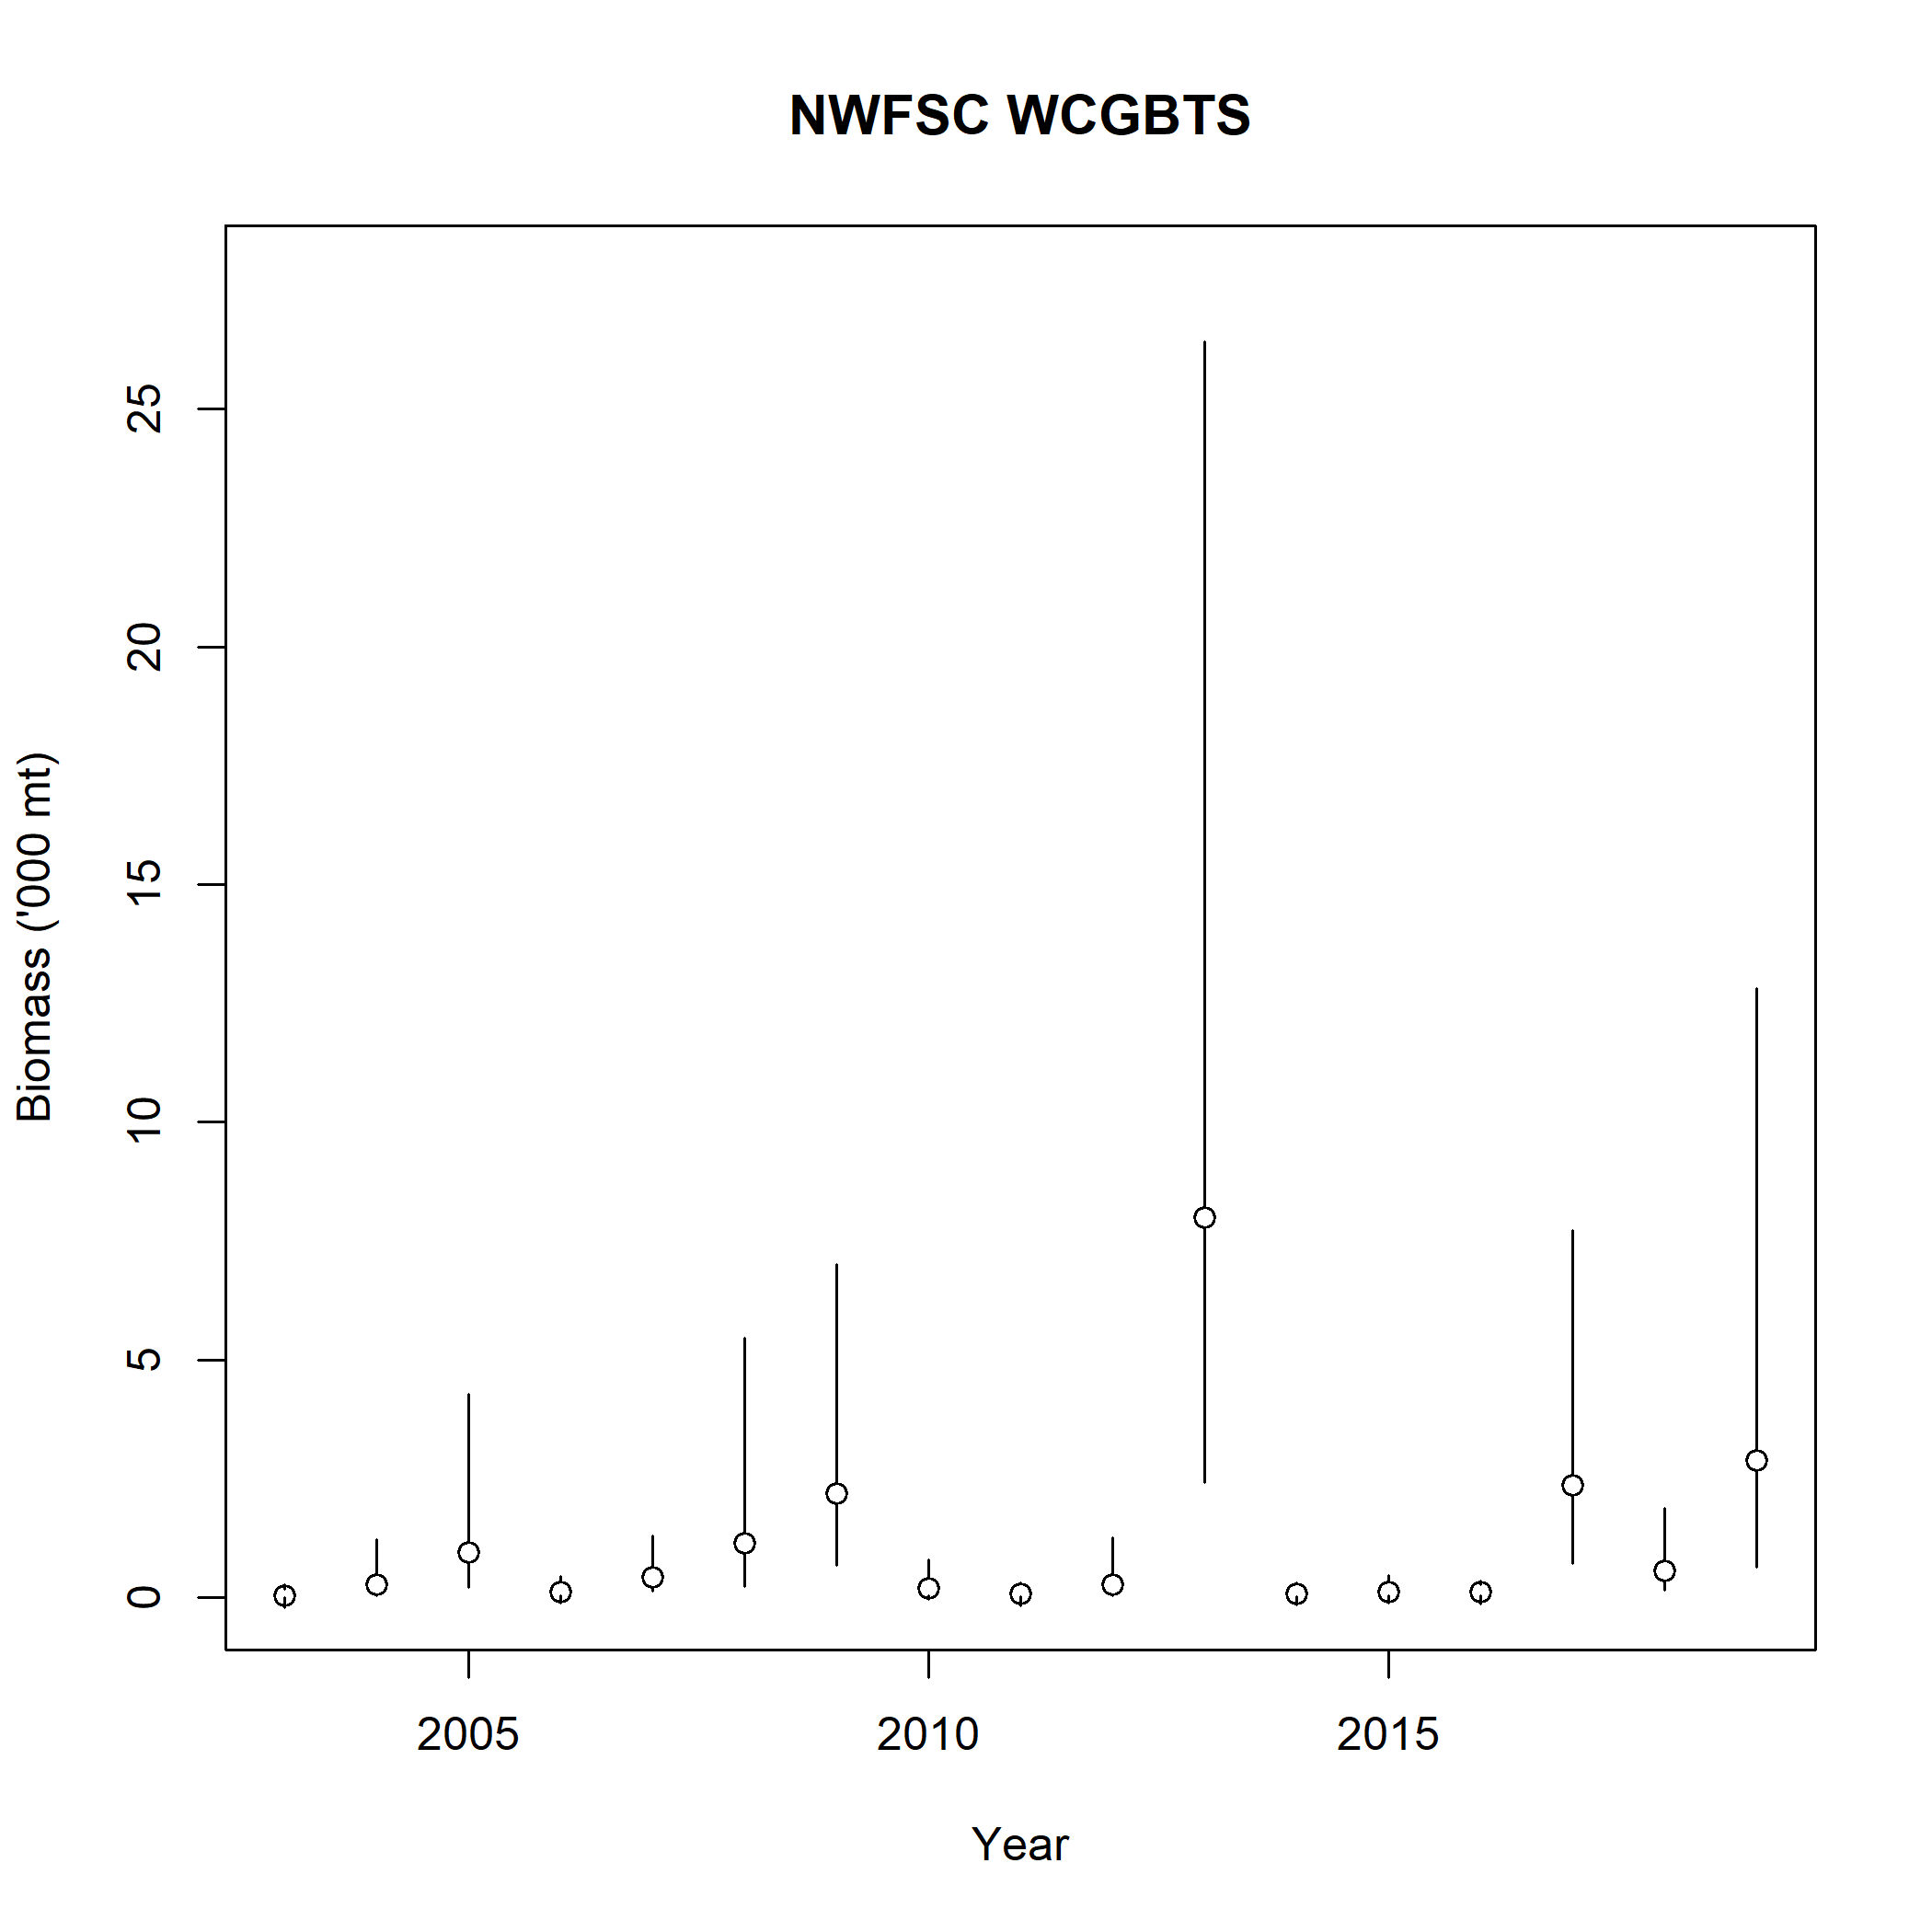
\includegraphics[width=1\textwidth,height=1\textheight]{//nwcfile/FRAM/Assessments/CurrentAssessments/DataModerate_2021/Squarespot_Rockfish/data/Trawl Survey Catch/plots/NWFSC WCGBTS_designed_based_index.png}
\caption{Design-based index of abundance for the NWFSC WCGBT survey.\label{fig:wcgbts-dbindex}}
\end{figure}

\tagmcend\tagstructend

\tagstructbegin{tag=Figure,alttext={Survey length-at-weight data with sex specific estimated fits and comparison to literature length-at-weight values.}}\tagmcbegin{tag=Figure}

\begin{figure}
\centering
\includegraphics[width=1\textwidth,height=1\textheight]{//nwcfile/FRAM/Assessments/CurrentAssessments/DataModerate_2021/Squarespot_Rockfish/data/biology/plots/Length_Weight_All_w_Love_Ests.png}
\caption{Survey length-at-weight data with sex specific estimated fits and comparison to literature length-at-weight values.\label{fig:len-weight}}
\end{figure}

\tagmcend\tagstructend

\tagstructbegin{tag=Figure,alttext={Observed length-at-age by data source.}}\tagmcbegin{tag=Figure}

\begin{figure}
\centering
\includegraphics[width=1\textwidth,height=1\textheight]{//nwcfile/FRAM/Assessments/CurrentAssessments/DataModerate_2021/Squarespot_Rockfish/data/biology/plots/doc_Data_Length_Age_by_Source.png}
\caption{Observed length-at-age by data source.\label{fig:len-age-data}}
\end{figure}

\tagmcend\tagstructend

\tagstructbegin{tag=Figure,alttext={Length-at-age estimated from the NWFSC WCGBT and Hook and Line survey data with sex specific estimated growth.}}\tagmcbegin{tag=Figure}

\begin{figure}
\centering
\includegraphics[width=1\textwidth,height=1\textheight]{//nwcfile/FRAM/Assessments/CurrentAssessments/DataModerate_2021/Squarespot_Rockfish/data/biology/plots/doc_Length_Age_by_Sex_RE.png}
\caption{Length-at-age estimated from the NWFSC WCGBT and Hook and Line survey data with sex specific estimated growth.\label{fig:len-age}}
\end{figure}

\tagmcend\tagstructend

\tagstructbegin{tag=Figure,alttext={Length at age in the beginning of the year in the ending year of the model.}}\tagmcbegin{tag=Figure}

\begin{figure}
\centering
\includegraphics[width=1\textwidth,height=1\textheight]{//nwcfile/FRAM/Assessments/CurrentAssessments/DataModerate_2021/Squarespot_Rockfish/models/Reference model/plots/bio1_sizeatage.png}
\caption{Length at age in the beginning of the year in the ending year of the model.\label{fig:len-age-ss}}
\end{figure}

\tagmcend\tagstructend

\tagstructbegin{tag=Figure,alttext={Maturity as a function of  length.}}\tagmcbegin{tag=Figure}

\begin{figure}
\centering
\includegraphics[width=1\textwidth,height=1\textheight]{//nwcfile/FRAM/Assessments/CurrentAssessments/DataModerate_2021/Squarespot_Rockfish/models/Reference model/plots/bio6_maturity.png}
\caption{Maturity as a function of length.\label{fig:maturity}}
\end{figure}

\tagmcend\tagstructend

\tagstructbegin{tag=Figure,alttext={Fecundity as a function of length.}}\tagmcbegin{tag=Figure}

\begin{figure}
\centering
\includegraphics[width=1\textwidth,height=1\textheight]{//nwcfile/FRAM/Assessments/CurrentAssessments/DataModerate_2021/Squarespot_Rockfish/models/Reference model/plots/bio9_fecundity_len.png}
\caption{Fecundity as a function of length.\label{fig:fecundity}}
\end{figure}

\tagmcend\tagstructend

\tagstructbegin{tag=Figure,alttext={Estimates of natural mortality for $S. hopkinsi$ using longevity = 45 years and female VBGF parameters. Error bars are based on a lognormal distribution with SD = 0.2.}}\tagmcbegin{tag=Figure}

\begin{figure}
\centering
\includegraphics[width=1\textwidth,height=1\textheight]{//nwcfile/FRAM/Assessments/CurrentAssessments/DataModerate_2021/Squarespot_Rockfish/data/biology/plots/Mplots2021-03-26_09_05_49_Female.png}
\caption{Estimates of natural mortality for {\tagstructbegin{tag=Formula}\tagmcbegin{tag=Formula}\(S. hopkinsi\)\leavevmode\tagmcend\tagstructend} using longevity = 45 years and female VBGF parameters. Error bars are based on a lognormal distribution with SD = 0.2.\label{fig:M_female}}
\end{figure}

\tagmcend\tagstructend

\tagstructbegin{tag=Figure,alttext={Composite natural mortality distriubtion for $S. hopkinsi$ using four longevity estimators each with a SD = 0.2 presuming a lognomral error distibution.}}\tagmcbegin{tag=Figure}

\begin{figure}
\centering
\includegraphics[width=1\textwidth,height=1\textheight]{//nwcfile/FRAM/Assessments/CurrentAssessments/DataModerate_2021/Squarespot_Rockfish/data/biology/plots/Mdensityplots_FishLife_longevity.png}
\caption{Composite natural mortality distriubtion for {\tagstructbegin{tag=Formula}\tagmcbegin{tag=Formula}\(S. hopkinsi\)\leavevmode\tagmcend\tagstructend} using four longevity estimators each with a SD = 0.2 presuming a lognomral error distibution.\label{fig:M_composite_dists}}
\end{figure}

\tagmcend\tagstructend

\tagstructbegin{tag=Figure,alttext={Selectivity at length by fleet.}}\tagmcbegin{tag=Figure}

\begin{figure}
\centering
\includegraphics[width=1\textwidth,height=1\textheight]{//nwcfile/FRAM/Assessments/CurrentAssessments/DataModerate_2021/Squarespot_Rockfish/models/Reference model/plots/sel01_multiple_fleets_length1.png}
\caption{Selectivity at length by fleet.\label{fig:selex}}
\end{figure}

\tagmcend\tagstructend

\tagstructbegin{tag=Figure,alttext={Jitter runs for the squarespot rockfish reference model, with jitter run number on the x-axis and -log likelihood value on the y-axis. Blue dot are models that match the likelihood value of the reference model, while red dots deviate from the reference model. All red dots are above the blue dots, indicating no better fit to the reference model was found.}}\tagmcbegin{tag=Figure}

\begin{figure}
\centering
\includegraphics[width=1\textwidth,height=1\textheight]{//nwcfile/FRAM/Assessments/CurrentAssessments/DataModerate_2021/Squarespot_Rockfish/models/Reference model/Jitter Results/jitterplot.png}
\caption{Jitter runs for the squarespot rockfish reference model, with jitter run number on the x-axis and -log likelihood value on the y-axis. Blue dot are models that match the likelihood value of the reference model, while red dots deviate from the reference model. All red dots are above the blue dots, indicating no better fit to the reference model was found.\label{fig:jitter_01}}
\end{figure}

\tagmcend\tagstructend

\tagstructbegin{tag=Figure,alttext={Pearson residuals for combind recreational and commercial fleet. Closed bubble are positive residuals (observed > expected) and open bubbles are negative residuals (observed < expected).}}\tagmcbegin{tag=Figure}

\begin{figure}
\centering
\includegraphics[width=1\textwidth,height=1\textheight]{//nwcfile/FRAM/Assessments/CurrentAssessments/DataModerate_2021/Squarespot_Rockfish/models/Reference model/plots/comp_lenfit_residsflt1mkt0_page3.png}
\caption{Pearson residuals for combind recreational and commercial fleet. Closed bubble are positive residuals (observed \textgreater{} expected) and open bubbles are negative residuals (observed \textless{} expected).\label{fig:rec-com-pearson}}
\end{figure}

\tagmcend\tagstructend

\tagstructbegin{tag=Figure,alttext={Mean length for combined recreational and commercial lengths with 95 percent confidence intervals based on current samples sizes.}}\tagmcbegin{tag=Figure}

\begin{figure}
\centering
\includegraphics[width=1\textwidth,height=1\textheight]{//nwcfile/FRAM/Assessments/CurrentAssessments/DataModerate_2021/Squarespot_Rockfish/models/Reference model/plots/comp_lenfit_data_weighting_TA1.8_Comm_Rec.png}
\caption{Mean length for combined recreational and commercial lengths with 95 percent confidence intervals based on current samples sizes.\label{fig:rec-com-mean-len-fit}}
\end{figure}

\tagmcend\tagstructend

\tagstructbegin{tag=Figure,alttext={Pearson residuals for NWFSC Hook and Line survey. Closed bubble are positive residuals (observed > expected) and open bubbles are negative residuals (observed < expected).}}\tagmcbegin{tag=Figure}

\begin{figure}
\centering
\includegraphics[width=1\textwidth,height=1\textheight]{//nwcfile/FRAM/Assessments/CurrentAssessments/DataModerate_2021/Squarespot_Rockfish/models/Reference model/plots/comp_lenfit_residsflt2mkt0.png}
\caption{Pearson residuals for NWFSC Hook and Line survey. Closed bubble are positive residuals (observed \textgreater{} expected) and open bubbles are negative residuals (observed \textless{} expected).\label{fig:hkl-pearson}}
\end{figure}

\tagmcend\tagstructend

\tagstructbegin{tag=Figure,alttext={Mean length for NWFSC Hook and Line survey lengths with 95 percent confidence intervals based on current samples sizes.}}\tagmcbegin{tag=Figure}

\begin{figure}
\centering
\includegraphics[width=1\textwidth,height=1\textheight]{//nwcfile/FRAM/Assessments/CurrentAssessments/DataModerate_2021/Squarespot_Rockfish/models/Reference model/plots/comp_lenfit_data_weighting_TA1.8_HKL.png}
\caption{Mean length for NWFSC Hook and Line survey lengths with 95 percent confidence intervals based on current samples sizes.\label{fig:hkl-mean-len-fit}}
\end{figure}

\tagmcend\tagstructend

\tagstructbegin{tag=Figure,alttext={Aggregated length comps over all years.}}\tagmcbegin{tag=Figure}

\begin{figure}
\centering
\includegraphics[width=1\textwidth,height=1\textheight]{//nwcfile/FRAM/Assessments/CurrentAssessments/DataModerate_2021/Squarespot_Rockfish/models/Reference model/plots/comp_lenfit__aggregated_across_time.png}
\caption{Aggregated length comps over all years.\label{fig:agg-len-fit}}
\end{figure}

\tagmcend\tagstructend

\tagstructbegin{tag=Figure,alttext={Fit to the NWFSC Hook and Line survey index of abundance.}}\tagmcbegin{tag=Figure}

\begin{figure}
\centering
\includegraphics[width=1\textwidth,height=1\textheight]{//nwcfile/FRAM/Assessments/CurrentAssessments/DataModerate_2021/Squarespot_Rockfish/models/Reference model/plots/index2_cpuefit_HKL.png}
\caption{Fit to the NWFSC Hook and Line survey index of abundance.\label{fig:hkl-index-fit}}
\end{figure}

\tagmcend\tagstructend

\tagstructbegin{tag=Figure,alttext={Estimated time series of spawning output.}}\tagmcbegin{tag=Figure}

\begin{figure}
\centering
\includegraphics[width=1\textwidth,height=1\textheight]{//nwcfile/FRAM/Assessments/CurrentAssessments/DataModerate_2021/Squarespot_Rockfish/models/Reference model/plots/ts7_Spawning_output_with_95_asymptotic_intervals_intervals.png}
\caption{Estimated time series of spawning output.\label{fig:ssb}}
\end{figure}

\tagmcend\tagstructend

\tagstructbegin{tag=Figure,alttext={Estimated time series of total biomass.}}\tagmcbegin{tag=Figure}

\begin{figure}
\centering
\includegraphics[width=1\textwidth,height=1\textheight]{//nwcfile/FRAM/Assessments/CurrentAssessments/DataModerate_2021/Squarespot_Rockfish/models/Reference model/plots/ts1_Total_biomass_(mt).png}
\caption{Estimated time series of total biomass.\label{fig:tot-bio}}
\end{figure}

\tagmcend\tagstructend

\tagstructbegin{tag=Figure,alttext={Estimated time series of fraction of unfished spawning output.}}\tagmcbegin{tag=Figure}

\begin{figure}
\centering
\includegraphics[width=1\textwidth,height=1\textheight]{//nwcfile/FRAM/Assessments/CurrentAssessments/DataModerate_2021/Squarespot_Rockfish/models/Reference model/plots/ts9_Relative_spawning_output_intervals.png}
\caption{Estimated time series of fraction of unfished spawning output.\label{fig:depl}}
\end{figure}

\tagmcend\tagstructend

\tagstructbegin{tag=Figure,alttext={Stock-recruit curve. Point colors indicate year, with warmer colors indicating earlier years and cooler colors in showing later years.}}\tagmcbegin{tag=Figure}

\begin{figure}
\centering
\includegraphics[width=1\textwidth,height=1\textheight]{//nwcfile/FRAM/Assessments/CurrentAssessments/DataModerate_2021/Squarespot_Rockfish/models/Reference model/plots/SR_curve.png}
\caption{Stock-recruit curve. Point colors indicate year, with warmer colors indicating earlier years and cooler colors in showing later years.\label{fig:bh-curve}}
\end{figure}

\tagmcend\tagstructend

\tagstructbegin{tag=Figure,alttext={Estimated time series of age-0 recruits (1000s).}}\tagmcbegin{tag=Figure}

\begin{figure}
\centering
\includegraphics[width=1\textwidth,height=1\textheight]{//nwcfile/FRAM/Assessments/CurrentAssessments/DataModerate_2021/Squarespot_Rockfish/models/Reference model/plots/ts11_Age-0_recruits_(1000s)_with_95_asymptotic_intervals.png}
\caption{Estimated time series of age-0 recruits (1000s).\label{fig:recruits}}
\end{figure}

\tagmcend\tagstructend

\tagstructbegin{tag=Figure,alttext={Estimated 1 - relative spawning ratio (SPR) by year.}}\tagmcbegin{tag=Figure}

\begin{figure}
\centering
\includegraphics[width=1\textwidth,height=1\textheight]{//nwcfile/FRAM/Assessments/CurrentAssessments/DataModerate_2021/Squarespot_Rockfish/models/Reference model/plots/SPR2_minusSPRseries.png}
\caption{Estimated 1 - relative spawning ratio (SPR) by year.\label{fig:1-spr}}
\end{figure}

\tagmcend\tagstructend

\tagstructbegin{tag=Figure,alttext={Equilibrium yield curve for the base case model. Values are based on the 2020 fishery selectivity and with steepness fixed at 0.72.}}\tagmcbegin{tag=Figure}

\begin{figure}
\centering
\includegraphics[width=1\textwidth,height=1\textheight]{//nwcfile/FRAM/Assessments/CurrentAssessments/DataModerate_2021/Squarespot_Rockfish/models/Reference model/plots/yield2_yield_curve_with_refpoints.png}
\caption{Equilibrium yield curve for the base case model. Values are based on the 2020 fishery selectivity and with steepness fixed at 0.72.\label{fig:yield}}
\end{figure}

\tagmcend\tagstructend

\tagstructbegin{tag=Figure,alttext={Log relative change (log((Model_sensi-Model_ref)/Model_ref) in data treatment for 5 derived quantities. Colored boxes indicate 95 percent confidence interval of the reference model.}}\tagmcbegin{tag=Figure}

\begin{figure}
\centering
\includegraphics[width=1\textwidth,height=1\textheight]{//nwcfile/FRAM/Assessments/CurrentAssessments/DataModerate_2021/Squarespot_Rockfish/models/_sensitivities/_plots/Data_sensis/Sensi_logREplot_SB_Dep_F_MSY.png}
\caption{Log relative change (log((Model\_sensi-Model\_ref)/Model\_ref) in data treatment for 5 derived quantities. Colored boxes indicate 95 percent confidence interval of the reference model.\label{fig:sensi-data-RE}}
\end{figure}

\tagmcend\tagstructend

\tagstructbegin{tag=Figure,alttext={Spawning biomass time series by data treatment compared to the reference model.}}\tagmcbegin{tag=Figure}

\begin{figure}
\centering
\includegraphics[width=1\textwidth,height=1\textheight]{//nwcfile/FRAM/Assessments/CurrentAssessments/DataModerate_2021/Squarespot_Rockfish/models/_sensitivities/_plots/Data_sensis/compare2_spawnbio_uncertainty.png}
\caption{Spawning biomass time series by data treatment compared to the reference model.\label{fig:sensi-data-ssb}}
\end{figure}

\tagmcend\tagstructend

\tagstructbegin{tag=Figure,alttext={Relative spawning biomass time series by data treatment compared to the reference model.}}\tagmcbegin{tag=Figure}

\begin{figure}
\centering
\includegraphics[width=1\textwidth,height=1\textheight]{//nwcfile/FRAM/Assessments/CurrentAssessments/DataModerate_2021/Squarespot_Rockfish/models/_sensitivities/_plots/Data_sensis/compare4_Bratio_uncertainty.png}
\caption{Relative spawning biomass time series by data treatment compared to the reference model.\label{fig:sensi-data-depl}}
\end{figure}

\tagmcend\tagstructend

\tagstructbegin{tag=Figure,alttext={Log relative change (log((Model_sensi-Model_ref)/Model_ref) in data treatment for 5 derived quantities. Colored boxes indicate 95 percent confidence interval of the reference model.}}\tagmcbegin{tag=Figure}

\begin{figure}
\centering
\includegraphics[width=1\textwidth,height=1\textheight]{//nwcfile/FRAM/Assessments/CurrentAssessments/DataModerate_2021/Squarespot_Rockfish/models/_sensitivities/_plots/Mod_specs/Sensi_logREplot_SB_Dep_F_MSY.png}
\caption{Log relative change (log((Model\_sensi-Model\_ref)/Model\_ref) in data treatment for 5 derived quantities. Colored boxes indicate 95 percent confidence interval of the reference model.\label{fig:sensi-modspec-RE}}
\end{figure}

\tagmcend\tagstructend

\tagstructbegin{tag=Figure,alttext={Spawning biomass time series by data treatment compared to the reference model.}}\tagmcbegin{tag=Figure}

\begin{figure}
\centering
\includegraphics[width=1\textwidth,height=1\textheight]{//nwcfile/FRAM/Assessments/CurrentAssessments/DataModerate_2021/Squarespot_Rockfish/models/_sensitivities/_plots/Mod_specs/compare2_spawnbio_uncertainty.png}
\caption{Spawning biomass time series by data treatment compared to the reference model.\label{fig:sensi-modspec-ssb}}
\end{figure}

\tagmcend\tagstructend

\tagstructbegin{tag=Figure,alttext={Relative spawning biomass time series by data treatment compared to the reference model.}}\tagmcbegin{tag=Figure}

\begin{figure}
\centering
\includegraphics[width=1\textwidth,height=1\textheight]{//nwcfile/FRAM/Assessments/CurrentAssessments/DataModerate_2021/Squarespot_Rockfish/models/_sensitivities/_plots/Mod_specs/compare4_Bratio_uncertainty.png}
\caption{Relative spawning biomass time series by data treatment compared to the reference model.\label{fig:sensi-modspec-depl}}
\end{figure}

\tagmcend\tagstructend

\tagstructbegin{tag=Figure,alttext={Asymptotic error in recruitment deviations when recruitment is estimated for all years. A drop in the asymptotic error (i.e., value approaches zero) is expected when data inform recruitment.}}\tagmcbegin{tag=Figure}

\begin{figure}
\centering
\includegraphics[width=1\textwidth,height=1\textheight]{//nwcfile/FRAM/Assessments/CurrentAssessments/DataModerate_2021/Squarespot_Rockfish/models/_sensitivities/_plots/sigmaR60_recdevs3_varcheck.png}
\caption{Asymptotic error in recruitment deviations when recruitment is estimated for all years. A drop in the asymptotic error (i.e., value approaches zero) is expected when data inform recruitment.\label{fig:rec-mod-var}}
\end{figure}

\tagmcend\tagstructend

\tagstructbegin{tag=Figure,alttext={$Log(R0)$ likelihood profiles (change in the negative log-likelihood across a range of $log(R0)$ values) and derived quantities (left four figures) and likelihood component contributions (right three figures). Red line in the top left most figure indicates the significance level in likelihood difference.}}\tagmcbegin{tag=Figure}

\begin{figure}
\centering
\includegraphics[width=1\textwidth,height=1\textheight]{//nwcfile/FRAM/Assessments/CurrentAssessments/DataModerate_2021/Squarespot_Rockfish/models/_likeprof/_profile_SR_LN(R0)/Profile_plots.png}
\caption{{\tagstructbegin{tag=Formula}\tagmcbegin{tag=Formula}\(Log(R0)\)\leavevmode\tagmcend\tagstructend} likelihood profiles (change in the negative log-likelihood across a range of {\tagstructbegin{tag=Formula}\tagmcbegin{tag=Formula}\(log(R0)\)\leavevmode\tagmcend\tagstructend} values) and derived quantities (left four figures) and likelihood component contributions (right three figures). Red line in the top left most figure indicates the significance level in likelihood difference.\label{fig:r0-profile-combo}}
\end{figure}

\tagmcend\tagstructend

\tagstructbegin{tag=Figure,alttext={Steepness likelihood profiles (change in the negative log-likelihood across a range of steepness values) and derived quantities (left four figures) and likelihood component contributions (right three figures).}}\tagmcbegin{tag=Figure}

\begin{figure}
\centering
\includegraphics[width=1\textwidth,height=1\textheight]{//nwcfile/FRAM/Assessments/CurrentAssessments/DataModerate_2021/Squarespot_Rockfish/models/_likeprof/_profile_SR_BH_steep/Profile_plots.png}
\caption{Steepness likelihood profiles (change in the negative log-likelihood across a range of steepness values) and derived quantities (left four figures) and likelihood component contributions (right three figures).\label{fig:steepness-profile-combo}}
\end{figure}

\tagmcend\tagstructend

\tagstructbegin{tag=Figure,alttext={Female $M$ likelihood profiles (change in the negative log-likelihood across a range of $M$ values) and derived quantities (left four figures) and likelihood component contributions (right three figures).}}\tagmcbegin{tag=Figure}

\begin{figure}
\centering
\includegraphics[width=1\textwidth,height=1\textheight]{//nwcfile/FRAM/Assessments/CurrentAssessments/DataModerate_2021/Squarespot_Rockfish/models/_likeprof/_profile_NatM_p_1_Fem_GP_1/Profile_plots.png}
\caption{Female {\tagstructbegin{tag=Formula}\tagmcbegin{tag=Formula}\(M\)\leavevmode\tagmcend\tagstructend} likelihood profiles (change in the negative log-likelihood across a range of {\tagstructbegin{tag=Formula}\tagmcbegin{tag=Formula}\(M\)\leavevmode\tagmcend\tagstructend} values) and derived quantities (left four figures) and likelihood component contributions (right three figures).\label{fig:M_f-profile-combo}}
\end{figure}

\tagmcend\tagstructend

\tagstructbegin{tag=Figure,alttext={Male $M$ likelihood profiles (change in the negative log-likelihood across a range of $M$ values) and derived quantities (left four figures) and likelihood component contributions (right three figures).}}\tagmcbegin{tag=Figure}

\begin{figure}
\centering
\includegraphics[width=1\textwidth,height=1\textheight]{//nwcfile/FRAM/Assessments/CurrentAssessments/DataModerate_2021/Squarespot_Rockfish/models/_likeprof/_profile_NatM_p_1_Mal_GP_1/Profile_plots.png}
\caption{Male {\tagstructbegin{tag=Formula}\tagmcbegin{tag=Formula}\(M\)\leavevmode\tagmcend\tagstructend} likelihood profiles (change in the negative log-likelihood across a range of {\tagstructbegin{tag=Formula}\tagmcbegin{tag=Formula}\(M\)\leavevmode\tagmcend\tagstructend} values) and derived quantities (left four figures) and likelihood component contributions (right three figures).\label{fig:M_m-profile-combo}}
\end{figure}

\tagmcend\tagstructend

\tagstructbegin{tag=Figure,alttext={Female and male $M$ multi-parameter likelihood profiles and derived quantities. Red lines in the top left figure indicate significantly similar values compared to the reference model. Broken and solid lines in the bottom right figure indicate target and limit referene points, respectively.}}\tagmcbegin{tag=Figure}

\begin{figure}
\centering
\includegraphics[width=1\textwidth,height=1\textheight]{//nwcfile/FRAM/Assessments/CurrentAssessments/DataModerate_2021/Squarespot_Rockfish/models/_likeprof/_profile_NatM_p_1_Fem_GP_1_NatM_p_1_Mal_GP_1/multilikelihood_profile.png}
\caption{Female and male {\tagstructbegin{tag=Formula}\tagmcbegin{tag=Formula}\(M\)\leavevmode\tagmcend\tagstructend} multi-parameter likelihood profiles and derived quantities. Red lines in the top left figure indicate significantly similar values compared to the reference model. Broken and solid lines in the bottom right figure indicate target and limit referene points, respectively.\label{fig:M-multiprofile-combo}}
\end{figure}

\tagmcend\tagstructend

\tagstructbegin{tag=Figure,alttext={Female $Linf$ likelihood profiles (change in the negative log-likelihood across a range of $L_inf$ values) and derived quantities (left four figures) and likelihood component contributions (right three figures).}}\tagmcbegin{tag=Figure}

\begin{figure}
\centering
\includegraphics[width=1\textwidth,height=1\textheight]{//nwcfile/FRAM/Assessments/CurrentAssessments/DataModerate_2021/Squarespot_Rockfish/models/_likeprof/_profile_L_at_Amax_Fem_GP_1/Profile_plots.png}
\caption{Female {\tagstructbegin{tag=Formula}\tagmcbegin{tag=Formula}\(Linf\)\leavevmode\tagmcend\tagstructend} likelihood profiles (change in the negative log-likelihood across a range of {\tagstructbegin{tag=Formula}\tagmcbegin{tag=Formula}\(L_inf\)\leavevmode\tagmcend\tagstructend} values) and derived quantities (left four figures) and likelihood component contributions (right three figures).\label{fig:Linf_F-profile-combo}}
\end{figure}

\tagmcend\tagstructend

\tagstructbegin{tag=Figure,alttext={Female $k$ likelihood profiles (change in the negative log-likelihood across a range of $k$ values) and derived quantities (left four figures) and likelihood component contributions (right three figures).}}\tagmcbegin{tag=Figure}

\begin{figure}
\centering
\includegraphics[width=1\textwidth,height=1\textheight]{//nwcfile/FRAM/Assessments/CurrentAssessments/DataModerate_2021/Squarespot_Rockfish/models/_likeprof/_profile_VonBert_K_Fem_GP_1/Profile_plots.png}
\caption{Female {\tagstructbegin{tag=Formula}\tagmcbegin{tag=Formula}\(k\)\leavevmode\tagmcend\tagstructend} likelihood profiles (change in the negative log-likelihood across a range of {\tagstructbegin{tag=Formula}\tagmcbegin{tag=Formula}\(k\)\leavevmode\tagmcend\tagstructend} values) and derived quantities (left four figures) and likelihood component contributions (right three figures).\label{fig:k_f-profile-combo}}
\end{figure}

\tagmcend\tagstructend

\tagstructbegin{tag=Figure,alttext={Female $Linf$ and $k$ multi-parameter likelihood profiles and derived quantities. Red lines in the top left figure indicate significantly similar values compared to the reference model. Broken and solid lines in the bottom right figure indicate target and limit referene points, respectively.}}\tagmcbegin{tag=Figure}

\begin{figure}
\centering
\includegraphics[width=1\textwidth,height=1\textheight]{//nwcfile/FRAM/Assessments/CurrentAssessments/DataModerate_2021/Squarespot_Rockfish/models/_likeprof/_profile_L_at_Amax_Fem_GP_1_VonBert_K_Fem_GP_1/multilikelihood_profile.png}
\caption{Female {\tagstructbegin{tag=Formula}\tagmcbegin{tag=Formula}\(Linf\)\leavevmode\tagmcend\tagstructend} and {\tagstructbegin{tag=Formula}\tagmcbegin{tag=Formula}\(k\)\leavevmode\tagmcend\tagstructend} multi-parameter likelihood profiles and derived quantities. Red lines in the top left figure indicate significantly similar values compared to the reference model. Broken and solid lines in the bottom right figure indicate target and limit referene points, respectively.\label{fig:Linf_k_f-profile}}
\end{figure}

\tagmcend\tagstructend

\tagstructbegin{tag=Figure,alttext={Female variability at maximum age likelihood profiles (change in the negative log-likelihood across a range of CV at maximum age values) and derived quantities (left four figures) and likelihood component contributions (right three figures).}}\tagmcbegin{tag=Figure}

\begin{figure}
\centering
\includegraphics[width=1\textwidth,height=1\textheight]{//nwcfile/FRAM/Assessments/CurrentAssessments/DataModerate_2021/Squarespot_Rockfish/models/_likeprof/_profile_CV_old_Fem_GP_1/Profile_plots.png}
\caption{Female variability at maximum age likelihood profiles (change in the negative log-likelihood across a range of CV at maximum age values) and derived quantities (left four figures) and likelihood component contributions (right three figures).\label{fig:CVold_f-profile-combo}}
\end{figure}

\tagmcend\tagstructend

\tagstructbegin{tag=Figure,alttext={Male $Linf$ likelihood profiles (change in the negative log-likelihood across a range of $L_inf$ values) and derived quantities (left four figures) and likelihood component contributions (right three figures).}}\tagmcbegin{tag=Figure}

\begin{figure}
\centering
\includegraphics[width=1\textwidth,height=1\textheight]{//nwcfile/FRAM/Assessments/CurrentAssessments/DataModerate_2021/Squarespot_Rockfish/models/_likeprof/_profile_L_at_Amax_Mal_GP_1/Profile_plots.png}
\caption{Male {\tagstructbegin{tag=Formula}\tagmcbegin{tag=Formula}\(Linf\)\leavevmode\tagmcend\tagstructend} likelihood profiles (change in the negative log-likelihood across a range of {\tagstructbegin{tag=Formula}\tagmcbegin{tag=Formula}\(L_inf\)\leavevmode\tagmcend\tagstructend} values) and derived quantities (left four figures) and likelihood component contributions (right three figures).\label{fig:Linf_M-profile-combo}}
\end{figure}

\tagmcend\tagstructend

\tagstructbegin{tag=Figure,alttext={Male $k$ likelihood profiles (change in the negative log-likelihood across a range of $k$ values) and derived quantities (left four figures) and likelihood component contributions (right three figures).}}\tagmcbegin{tag=Figure}

\begin{figure}
\centering
\includegraphics[width=1\textwidth,height=1\textheight]{//nwcfile/FRAM/Assessments/CurrentAssessments/DataModerate_2021/Squarespot_Rockfish/models/_likeprof/_profile_VonBert_K_Mal_GP_1/Profile_plots.png}
\caption{Male {\tagstructbegin{tag=Formula}\tagmcbegin{tag=Formula}\(k\)\leavevmode\tagmcend\tagstructend} likelihood profiles (change in the negative log-likelihood across a range of {\tagstructbegin{tag=Formula}\tagmcbegin{tag=Formula}\(k\)\leavevmode\tagmcend\tagstructend} values) and derived quantities (left four figures) and likelihood component contributions (right three figures).\label{fig:k_m-profile-combo}}
\end{figure}

\tagmcend\tagstructend

\tagstructbegin{tag=Figure,alttext={Male $L_inf$ and $k$ multi-parameter likelihood profiles and derived quantities. Red lines in the top left figure indicate significantly similar values compared to the reference model. Broken and solid lines in the bottom right figure indicate target and limit referene points, respectively.}}\tagmcbegin{tag=Figure}

\begin{figure}
\centering
\includegraphics[width=1\textwidth,height=1\textheight]{//nwcfile/FRAM/Assessments/CurrentAssessments/DataModerate_2021/Squarespot_Rockfish/models/_likeprof/_profile_L_at_Amax_Mal_GP_1_VonBert_K_Mal_GP_1/multilikelihood_profile.png}
\caption{Male {\tagstructbegin{tag=Formula}\tagmcbegin{tag=Formula}\(L_inf\)\leavevmode\tagmcend\tagstructend} and {\tagstructbegin{tag=Formula}\tagmcbegin{tag=Formula}\(k\)\leavevmode\tagmcend\tagstructend} multi-parameter likelihood profiles and derived quantities. Red lines in the top left figure indicate significantly similar values compared to the reference model. Broken and solid lines in the bottom right figure indicate target and limit referene points, respectively.\label{fig:Linf_k_m-profile}}
\end{figure}

\tagmcend\tagstructend

\tagstructbegin{tag=Figure,alttext={Male variability at maximum age likelihood profiles (change in the negative log-likelihood across a range of CV at maximum age values) and derived quantities (left four figures) and likelihood component contributions (right three figures).}}\tagmcbegin{tag=Figure}

\begin{figure}
\centering
\includegraphics[width=1\textwidth,height=1\textheight]{//nwcfile/FRAM/Assessments/CurrentAssessments/DataModerate_2021/Squarespot_Rockfish/models/_likeprof/_profile_CV_old_Mal_GP_1/Profile_plots.png}
\caption{Male variability at maximum age likelihood profiles (change in the negative log-likelihood across a range of CV at maximum age values) and derived quantities (left four figures) and likelihood component contributions (right three figures).\label{fig:CVold_m-profile-combo}}
\end{figure}

\tagmcend\tagstructend

\tagstructbegin{tag=Figure,alttext={Change in the estimate of spawning output when the most recent 10 years of data area removed sequentially.}}\tagmcbegin{tag=Figure}

\begin{figure}
\centering
\includegraphics[width=1\textwidth,height=1\textheight]{//nwcfile/FRAM/Assessments/CurrentAssessments/DataModerate_2021/Squarespot_Rockfish/models/_retro//compare2_spawnbio_uncertainty.png}
\caption{Change in the estimate of spawning output when the most recent 10 years of data area removed sequentially.\label{fig:retro-ssb}}
\end{figure}

\tagmcend\tagstructend

\tagstructbegin{tag=Figure,alttext={Change in the estimate of fraction unfished when the most recent 10 years of data area removed sequentially.}}\tagmcbegin{tag=Figure}

\begin{figure}
\centering
\includegraphics[width=1\textwidth,height=1\textheight]{//nwcfile/FRAM/Assessments/CurrentAssessments/DataModerate_2021/Squarespot_Rockfish/models/_retro//compare4_Bratio_uncertainty.png}
\caption{Change in the estimate of fraction unfished when the most recent 10 years of data area removed sequentially.\label{fig:retro-depl}}
\end{figure}

\tagmcend\tagstructend

\newpage

\clearpage

\tagstructbegin{tag=H1}\tagmcbegin{tag=H1}

\hypertarget{appendix-a.-summary-of-california-management-measures}{%
\section{Appendix A. Summary of California Management Measures}\label{appendix-a.-summary-of-california-management-measures}}

\leavevmode\tagmcend\tagstructend

\tagstructbegin{tag=P}\tagmcbegin{tag=P}

Appendix A can be found in the separate file ``California Nearshore Regulation History.pdf.''

\leavevmode\tagmcend\tagstructend\par

\tagstructbegin{tag=H1}\tagmcbegin{tag=H1}

\hypertarget{appendix-b.-detailed-fit-to-length-composition-data}{%
\section{Appendix B. Detailed Fit to Length Composition Data}\label{appendix-b.-detailed-fit-to-length-composition-data}}

\leavevmode\tagmcend\tagstructend

\tagstructbegin{tag=Figure,alttext={Length comps, whole catch, Comm_Rec (plot 1 of 3).<br><br>'N adj.' is the input sample size after data-weighting adjustment. N eff. is the calculated effective sample size used in the McAllister-Iannelli tuning method..}}\tagmcbegin{tag=Figure}

\begin{figure}
\centering
\includegraphics[width=1\textwidth,height=1\textheight]{//nwcfile/FRAM/Assessments/CurrentAssessments/DataModerate_2021/Squarespot_Rockfish/models/Reference model/plots/comp_lenfit_flt1mkt0_page1.png}
\caption{Length comps, whole catch, Comm\_Rec (plot 1 of 3).`N adj.' is the input sample size after data-weighting adjustment. N eff. is the calculated effective sample size used in the McAllister-Iannelli tuning method..\label{fig:comp_lenfit_flt1mkt0_page1}}
\end{figure}

\tagmcend\tagstructend

\tagstructbegin{tag=Figure,alttext={Length comps, whole catch, Comm_Rec (plot 2 of 3).}}\tagmcbegin{tag=Figure}

\begin{figure}
\centering
\includegraphics[width=1\textwidth,height=1\textheight]{//nwcfile/FRAM/Assessments/CurrentAssessments/DataModerate_2021/Squarespot_Rockfish/models/Reference model/plots/comp_lenfit_flt1mkt0_page2.png}
\caption{Length comps, whole catch, Comm\_Rec (plot 2 of 3).\label{fig:comp_lenfit_flt1mkt0_page2}}
\end{figure}

\tagmcend\tagstructend

\tagstructbegin{tag=Figure,alttext={Length comps, whole catch, Comm_Rec (plot 3 of 3).}}\tagmcbegin{tag=Figure}

\begin{figure}
\centering
\includegraphics[width=1\textwidth,height=1\textheight]{//nwcfile/FRAM/Assessments/CurrentAssessments/DataModerate_2021/Squarespot_Rockfish/models/Reference model/plots/comp_lenfit_flt1mkt0_page3.png}
\caption{Length comps, whole catch, Comm\_Rec (plot 3 of 3).\label{fig:comp_lenfit_flt1mkt0_page3}}
\end{figure}

\tagmcend\tagstructend

\tagstructbegin{tag=Figure,alttext={Length comps, whole catch, HKL.<br><br>'N adj.' is the input sample size after data-weighting adjustment. N eff. is the calculated effective sample size used in the McAllister-Iannelli tuning method..}}\tagmcbegin{tag=Figure}

\begin{figure}
\centering
\includegraphics[width=1\textwidth,height=1\textheight]{//nwcfile/FRAM/Assessments/CurrentAssessments/DataModerate_2021/Squarespot_Rockfish/models/Reference model/plots/comp_lenfit_flt2mkt0.png}
\caption{Length comps, whole catch, HKL.`N adj.' is the input sample size after data-weighting adjustment. N eff. is the calculated effective sample size used in the McAllister-Iannelli tuning method..\label{fig:comp_lenfit_flt2mkt0}}
\end{figure}

\tagmcend\tagstructend
\end{document}
